\documentclass[11pt, a4paper]{memoir}
\let\printglossary\relax
\let\theglossary\relax
\let\endtheglossary\relax
\usepackage[english, sund, dropcaps, hyperref, submissionstatement]{ku-frontpage}
\usepackage[utf8]{inputenc}
\usepackage[dvipsnames,rgb]{xcolor}
\usepackage[T1]{fontenc}
\usepackage{amsmath}
\usepackage{mathptmx}
\usepackage{enumitem}
\usepackage{lipsum}
\usepackage{pdfpages}

% Figures
\usepackage[export]{adjustbox}
\usepackage{graphicx}
\usepackage[caption=false, position=top]{subfig}
\captionsetup[subfloat]{font={bf}, skip=1pt, singlelinecheck=false}

% tikz
\usepackage{tikz}
\usetikzlibrary{arrows.meta, decorations.pathmorphing, decorations.pathreplacing, positioning, shapes.geometric}
\tikzset{every picture/.style={/utils/exec={\sffamily}}}

% Glossary
\usepackage{glossaries}
\makenoidxglossaries
\loadglsentries{0E_Abbreviations.tex}

% Margins
\setlength\parskip{1em}
\setlength\arraycolsep{2 pt}
\setcounter{tocdepth}{2}
\setcounter{secnumdepth}{2}
\setlrmarginsandblock{2.5cm}{2.5cm}{*}
\setulmarginsandblock{2.5cm}{2.5cm}{*}
\OnehalfSpacing
\checkandfixthelayout

\assignment{PhD thesis}
\frontpageauthor{Neil Alexandre Scheidwasser}

% The following are only needed if the \author, \title, \subtitle, and \date
% commands are not patchable. See the readme for more information.
% \frontpageauthor{Alex Author}
% \frontpagetitle{A concise but nevertheless\\precise and interesting title}
% \frontpagesubtitle{An intruiging subtitle}
% \frontpagedate{Submitted: \today}

\frontpagetitle{Pandemic preparedness in a vector}
\subtitle{How new representations of data from phylogenetic trees, protein structures, and animal tracking can help understand pandemics}
\frontpagedate{Submitted: \today}
\advisor{Principal supervisor: Samir Bhatt}
\coadvisor{Co-supervisor: David Duchêne}
\frontpageimage{example.png}

\kupdfsetup{}{}{Neil Alexandre Scheidwasser}

\renewcommand*\contentsname{Table of Contents}

\usepackage[style=nature, autocite=superscript, natbib=true, uniquename=init]{biblatex}
\addbibresource{References.bib}
\renewcommand{\cite}{\autocite}

%% ======= New commands =======
% Phylo2Vec vector
\renewcommand{\v}{$\boldsymbol{v}$}
% Semibold font
\DeclareRobustCommand{\sbseries}{\fontseries{sb}\selectfont}
\DeclareTextFontCommand{\textsb}{\sbseries}

\begin{document}
\begingroup
  \fontencoding{T1}\fontfamily{LinuxLibertineT-OsF}\selectfont
  \maketitle
\endgroup

\section*{Abstract}
\input{0A_Abstract}
\clearpage
\section*{Dansk Resumé}
COVID-19 pandemien er et bevis på, hvor komplekst det er at forberede sig og reagere på udbrud af smitsomme sygdomme. Ud fra et styringsmæssigt perspektiv krævede det koordinerede nationale og internationale indsatser. Ud fra et logistik perspektiv krævede det modstandsdygtige forsyningskæder for at distribuere medicinsk udstyr og vacciner. Ud fra et videnskabeligt perspektiv krævede det indsatser uden fortilfælde i størrelse og omfang til genomisk testning, sekvensering og modellering for at undersøge hvor virussen spredte sig og udviklede sig. Dog vil en omfattende reaktion mod sygdomsudbrud ikke afhænge af storstilet genomisk overvågning alene. Et godt eksempel er registerdata i Danmark, som var væsentlig for at afsløre regionale og demografiske mønstre af infektion. Under disse forudsætninger kan andre typer af data hjælpe at fremsætte værdifulde indsigter til udbrudsdynamik. Disse kan inkludere molekylære data fra biofysiske interaktioner mellem patogen og receptorer i værtsorganismer. En anden mulighed er data om økologi af naturlige reservoirer, som man kan opnå med ikke-invasive overvågningssystemer. Den slags datatyper er meget komplekse og det at udvikle effektive dataanalytiske metoder er altafgørende for at oversætte data til indsigter, som man kan basere afgørelser på inden for rimelige tidsrammer. Denne afhandling undersøger, hvordan vores forståelse af pandemier kan forbedres ved hjælp af nye datarepræsentationer af fylogeni, proteinstruktur og dyreadfærd.

Først udviklede jeg phylo2vec, en matematisk vektorrepræsentation af binære fylogenetiske træer. Designet med et særligt fokus på effektiv generering og datakompression muliggør denne kompakte repræsentation skalerbar analyse af fylogenetiske data med moderne \textit{machine learning} metoder. I det andet studie ønskede jeg efter at udforske en anden datastrøm: proteinstrukturer. Ved hjælp af en ny diskret repræsentation af proteinstruktur undersøgte jeg de evolutionære processer, der ligger bag affinitet mellem \textit{Betacoronavirus} Spike glykoproteiner og værtsreceptorer. I en første analyse af proteinsekvenser fandt jeg, at brugen af den humane ACE2-receptor er forbundet med genetisk rekombination i S1 underenheden af proteinet og med mutation i det N-terminale domæne af S1. Samtidig tyder strukturelle data på, at receptorskift medieres gennem gradvise strukturelle forbedringer inden for receptorbinding snarere end konformationel reorganisering. I den tredje studie undersøgte jeg potentialet for at detektere tidlige infektionssignaturer hos slagtekyllinger ved hjælp af \textit{deep learning}-baseret dyresporing. Ved at bruge \textit{Escherichia coli}, en betydelig trusel i den danske fjerkræbranche, som modelpatogen, fandt jeg beviser for at denne teknik kan bruges til at måle adfærdsmønstre, som er forbundet med forringet velfærd. Dette resultat viser kunstig intelligens' potentiale for at automatisere omdannelse af videoovervågningsdata til kvantitative dyrevelfærdsmålinger og, alt i alt, drive effektive løsninger til epidemiovervågning i fjerkræpopulationer.

Samlet set illustrerer denne afhandling den iboende tværfaglige karakter af et beredskab for pandemier. Den viser, at forskellige datastrømme kan integreres i sundhedsinfrastrukturer via avanceret datateknik. Ud over konventionel genetisk og videobaseret overvågning vil nye analytiske metoder accelerere detektion og analyse af patogener og uddybe vores forståelse af nye trusler fra infektionssygdomme.

% In the third data stream, I investigated the feasibility of detecting early infection signatures in broiler chickens using deep learning-based animal tracking. Using \textit{Escherichia coli}, a major threat in poultry farming in Denmark, as a model pathogen, I found evidence that simple behavioural patterns tracked from videography are associated with impaired welfare. This result showcases the potential of artificial intelligence to power low-cost solutions for epidemic monitoring in poultry populations, enabling the automated transformation of video surveillance into quantitative animal welfare metrics.

% First, I developed phylo2vec, a mathematical integer vector representation of binary phylogenetic trees. Designed with efficient sampling and data storage in mind, this compact representation paves the way for scalable analysis of phylogenetic data using modern machine learning techniques. Exploring a second data stream, I used protein structures to investigate the evolutionary mechanisms underlying the affinity of \textit{Betacoronavirus} spike proteins to host receptors. By casting protein structures into a discrete representation, I found that the use of the human ACE2 receptor is linked with molecular recombination in the gene S1 subunit and with amino acid substitution rates in the N-terminal domain. Meanwhile, structural data suggest that receptor switching is mediated through gradual structural refinements within the receptor-binding domain rather than large-scale conformational reorganisation. In the third data stream, I investigated the feasibility of detecting early infection signatures in broiler chickens using deep learning-based animal tracking. Using \textit{Escherichia coli}, a major threat in poultry farming in Denmark, as a model pathogen, I found evidence that simple behavioural patterns tracked from videography are associated with impaired welfare. This result showcases the potential of artificial intelligence to power low-cost solutions for epidemic monitoring in poultry populations, enabling the automated transformation of video surveillance into quantitative animal welfare metrics.

% Ved at udforske en anden datastrøm har jeg omdannet proteinstrukturer til diskrete repræsentationer og brugt disse til at undersøge de evolutionære mekanismer, der ligger bag affinitet mellen antigener og værtsreceptorer. I en analyse af sekvensdata på aminosyrer af \textit{Betacoronavirus} spike glycoproteiner fandt jeg, at brugen af den humane ACE2-receptor er forbundet med molekylær rekombination i underenheden til genet S1 og med aminosyresubstitutionshastigheder i det N-terminale domæne. Samtidig tyder strukturelle data på, at receptorskift medieres gennem gradvise strukturelle forbedringer inden for receptorbinding snarere end storstilet konformationel reorganisering. I den tredje datastrøm undersøgte jeg muligheden for deep learning-baseret sporing af dyr for at detektere tidlige infektionssignaturer hos slagtekyllinger. Ved at bruge \textit{Escherichia coli}, en stor trussel i fjerkræavl i Danmark, som modelpatogen, fandt jeg beviser fra videooptagelser for, at simple adfærdsmønstre er forbundet med forringet velfærd. Dette placerer derfor computer vision som en kraftfuld og billig løsning til epidemiovervågning i fjerkræpopulationer via automatiseret omdannelse af videoovervågning til kvantitative adfærdsmålinger.

% Samlet set illustrerer denne afhandling den iboende tværfaglige karakter af et beredskab for pandemier. Den viser, at forskellige datastrømme kan integreres i sundhedsinfrastrukturer via avanceret datateknik. Ud over konventionel genetisk og videobaseret overvågning vil nye analytiske metoder accelerere detektion og analyse af patogener og uddybe vores forståelse af nye trusler fra infektionssygdomme.



% % Et beredskab for pandemier er en vigtig byggesten i den globale sundhedsinfrastruktur. Ud over logistiske og forvaltningsmæssige udfordringer kræver et robust beredskab en forskningsindsats på tværs af flere videnskabelige discipliner. Den seneste COVID-19-pandemi eksemplificerer denne kompleksitet og viser, at en omfattende respons på sygdomsudbrud muligvis ikke kun afhænger af omfattende testning for infektion. I stedet kan vi udvide vores forståelse af sygdomsudbrud betydeligt ved at inkludere komplementære datastrømme. Disse datastrømme kan omfatte data om udvikling af patogener på tværs af millioner af patienter, biofysiske interaktioner mellem patogener og værtsmolekyler samt ikke-invasive detektionssystemer i dyrereservoirer. Disse datatyper er yderst komplekse og udvikling af beregningsmæssigt effektive analysemetoder er afgørende for at omsætte data til brugbar indsigt inden for operationelt relevante tidsrammer. Denne afhandling undersøger, hvordan vores forståelse af pandemier kan forbedres ved hjælp af nye datarepræsentationer af fylogeni, proteinstruktur og dyreadfærd.


% \textbf{Things I am unsure of:
% }
% % - data streams: datastrømme? Not in the dictionary, but websites use it. https://ordnet.dk/ddo/ordbog?query=datastrømmen

% % - integer... the word heltalsvektorrepræsentation does not seem to exist even though google translate wants it to. I propose something without the interger part maybe? Or have it as a seperate word before. Now I have written "matematisk vektorrepræsentation af binære fylogenetiske træer" which is does not cover the interger part.

% % - discrete representation: diskrete repræsentationer? Should be fine but maybe ask Frederik? I cannot find anything on google on this in Danish Math things.

% % - governing antigen affinity to host receptors:  styrer affinitet mellen antigener og værtsreceptorer. Not 100 procent sure about this translation because of my lack of biology knowlegde.

% - amino acid substitution rates: aminosyresubstitutionshastigheder. This is the direct translation but does not seem to exist. Could be "substitionshastigheder for aminosyre".

% - data engeneering: datatektik. One of those words that might be better in english

% - also double check this sentence with someone with biology knowlegde: I en analyse af sekvensdata på aminosyrer af Betacoronavirus spike glycoproteiner fandt jeg, at brugen af den humane ACE2-receptor er forbundet med molekylær rekombination i underenheden til genet S1 og med aminosyresubstitutionshastigheder i det N-terminale domæne

% - last sentence: is it new treats or new diseases? The "nye" might need to be moved
\clearpage
\section*{Acknowledgements}
Sam, Swapnil for taking me in the lab, thankful for the support, insightful chats and coding sessions and great freedom

Mark, Johannes, Mathilde, Nicolas as great office mates

Mark, Jacob, Christian for COVID work

Alex for EWS work

Kathrine for taking me in the steering committee + GRASPH

All Danish colleagues for my annoying Danish language questions

Matt, Ayush, Madeline, Don for work of phylo, Prince, Louise, and Danny for work on chickens

David and Sam for supervision

Swapnil for conference in SG

Christian for exchange in London

Marianne, family, friends for moral support

DNRF, Novo, Carlsberg for funding
\clearpage
\section*{Scientific Contributions}
{\large
$^*$: equal contribution.
\noindent Included in this thesis:
\begin{enumerate}[noitemsep, topsep=0pt, leftmargin=*, align=left]
    \item[Study 1a.] Penn, M. J.$^*$, \textbf{Scheidwasser, N.}$^*$, Khurana, M. P., Duchêne, D. A., Donnelly, C. A., \& Bhatt, S. (2025). Phylo2Vec: a vector representation for binary trees. \textit{Systematic Biology}, \textbf{74}(2), 250-266. \doi{10.1093/sysbio/syae030}
    \item[Study 1b.] \textbf{Scheidwasser, N.}$^*$, Nag, A.$^*$, Penn, M. J., Jakob, A., Andersen, F. M., Khurana, M. P., Setiawan, L., Gordon, M., Duchêne D. A. \& Bhatt, S. (2025). phylo2vec: a library for vector-based phylogenetic tree manipulation. \textit{arXiv preprint arXiv:2506.19490}, \doi{10.48550/arXiv.2506.19490}. Under review at \textit{J. Open Source Softw.}. 
    \item[Study 2.] \textbf{Scheidwasser, N.}, Khurana, M. P., Morgenstern, C., Pust N., Leow P. R., Kavanagh R., Bhatt, S. \& Duchêne, D.A. (2025). Recombination of binding domains shapes structural evolution of \textit{Betacoronavirus} spike proteins, \textit{Manuscript}.
    \item[Study 3.] \textbf{Scheidwasser, N.}$^*$, Poulsen, L. L.$^*$, Leow, P. R., Khurana, M. P., Iglesias-Carrasco, M., Laydon, D. J., Donnelly, C. A., Bojesen, A. M. B., Bhatt S. \& Duchêne, D. A. (2025). Deep learning from videography as a tool for measuring \textit{E. coli} infection in poultry. \textit{Royal Society Open Science}, \textbf{12}(10), 250151. \doi{10.1098/rsos.250151}
\end{enumerate}
}

{\small
\noindent Not included in this thesis:
\begin{enumerate}[noitemsep, topsep=0pt, leftmargin=*]
    \item Coupland, H., \textbf{Scheidwasser, N.}, Katsiferis, A., Davies, M., Flaxman, S., Hulvej Rod, N., ... \& Unwin, H. J. T. (2025). Exploring the potential and limitations of deep learning and explainable AI for longitudinal life course analysis. \textit{BMC Public Health}, \textbf{25}(1), 1520.
    \item Kraemer, M. U., Tsui, J. L. H., Chang, S. Y., Lytras, S., Khurana, M. P., Vanderslott, S., Bajaj, S., \textbf{Scheidwasser, N.}, ... \& Bhatt, S. (2025). Artificial intelligence for modelling infectious disease epidemics. \textit{Nature}, \textbf{638}(8051), 623-635.
    \item Penn, M. J., \textbf{Scheidwasser, N.}, Donnelly, C. A., Duchêne, D. A., \& Bhatt, S. (2025). Bayesian inference of phylogenetic distances: revisiting the eigenvalue approach. \textit{Bulletin of Mathematical Biology}, \textbf{87}(2), 32.
    \item Khurana, M. P., \textbf{Scheidwasser, N.}, Penn, M. J., Bhatt, S., \& Duchêne, D. A. (2024). The limits of the constant-rate birth–death prior for phylogenetic tree topology inference. \textit{Systematic Biology}, \textbf{73}(1), 235-246.
    \item Khurana, M. P.$^*$, Curran-Sebastian, J.$^*$, \textbf{Scheidwasser, N.}$^*$, Morgenstern, C., Rasmussen, M., Fonager, J., ... \& Bhatt, S. (2024). High-resolution epidemiological landscape from 290,000 SARS-CoV-2 genomes from Denmark. \textit{Nature Communications}, 15(1), 7123.
    \item Wu, Z., \textbf{Scheidwasser-Clow, N.}, El Hajal, K., Cernak, M. (2023) Speaker Embeddings as Individuality Proxy for Voice Stress Detection. \textit{Proc. Interspeech}, 1838-1842.
    \item Penn, M. J.$^*$, \textbf{Scheidwasser, N.}$^*$, Penn, J., Donnelly, C. A., Duchêne, D. A., \& Bhatt, S. (2023). Leaping through tree space: continuous phylogenetic inference for rooted and unrooted trees. \textit{Genome Biology and Evolution}, \textbf{15}(12), evad213.
    \item El Hajal, K., Wu, Z., \textbf{Scheidwasser-Clow, N.}, Elbanna, G., \& Cernak, M. (2023). Efficient speech quality assessment using self-supervised framewise embeddings. In \textit{Proc. ICASSP} (pp. 1-5). IEEE.
\end{enumerate}
}
\clearpage
% \section*{Abbreviations}
\setglossarysection{section}
\printnoidxglossary[title=Abbreviations]
\clearpage

\tableofcontents

\chapter{Introduction}
Human history has been profoundly shaped by waves of pathogen-borne epidemics. They have left enduring marks on our species, ranging from our behaviour and social norms to our cellular and genetic material. A major factor of infectious disease outbreaks is our interactions with other animal species, which have become increasingly frequent with migration, domestication, and ecosystem-eroding technological advancements. Such interactions facilitate spillover events~\cite{vora2022, sikora2025}, in which a pathogen prevalent in a host animal reservoir is transmitted to a nearby human population. Although progress in science, medicine, and public health awareness has greatly mitigated the frequency and impact of \emph{zoonotic} epidemics, the acceleration of globalisation and climate change in the 21st century is likely to change the balance~\cite{carlson2022}. Indeed, recent estimates posit that a COVID-19-style pandemic is likely to occur once every 129 years on average~\cite{marani2021}. Among other factors, ecosystem modifications (e.g., deforestation, loss of biodiversity~\cite{ostfeld2009, keesing2010}) reduce buffers between zoonotic reservoirs and human populations, while global warming facilitates the geographical expansion of disease-carrying vectors such as bats, mosquitoes, and rodents~\cite{li2005, jones2008, ryan2019, johnson2020}. 

Since the early 2000s, global organisations such as the \gls{who} and the World Bank have spearheaded efforts such as the Global Outbreak Alert and Response Network (GOARN) and the Global Pandemic Monitoring Board (GPMB) to strengthen international pandemic coordination~\cite{heymann2001, knobler2004, who2025}. Yet, as illustrated by the recent COVID-19 pandemic, preparedness against such events remains a Herculean task. Beyond logistical and sociopolitical issues, the scientific landscape of \emph{pandemic preparedness} is inherently interdisciplinary~\cite{fefferman2023}. For instance, microbiology is paramount for deciphering the structure and function of pathogenic agents; ecology and veterinary science are essential for studying the dynamics of animal reservoirs; advanced statistics are needed for modelling the progress of epidemics; and information technology is crucial for developing efficient software. Nowadays, \emph{data science} has become a pillar of pandemic preparedness, as research in infectious disease epidemiology increasingly relies on the analysis of large-scale heterogeneous datasets~\cite{leonelli2021}. These include wildlife monitoring footage, pathogenic genomes from wastewater, human mobility patterns, and electronic health records. Moreover, a substantial body of research on the COVID-19 pandemic has highlighted the utility of large-scale, possibly population-wide, datasets to better understand the dynamics of disease transmission, identify risk factors, and inform effective prevention and intervention strategies~\cite{grenfell2004, robishaw2021, vigfusson2021, attwood2022, matteson2023, khurana2024}. Thus, investment in data-driven research is crucial for our preparedness for the next pandemic.

\newpage

This thesis aims to contribute to pandemic preparedness through advances in data science, in which a common underlying theme is the mathematical \emph{vectorisation} of pandemic-related data. Representing complex data in a simple array of numbers is desirable for efficient storage, scalability, and interoperability with various statistical frameworks. More specifically, I first introduce \emph{phylo2vec}~\cite{penn2025}, a method for encoding phylogenetic trees (a representation of evolutionary relationships between entities) into a simple integer-based vector. The primary objective of this method was to enable efficient data compression, rapid tree sampling and to facilitate the use of phylogenetic trees in comparative analyses and potential machine learning applications. The objective of the second study was to explore the potential of protein structures to complement our understanding of viral pathogen evolution. Whereas viral evolution is typically studied through sequence analysis, structures may offer new insight as a more direct reflection of protein function~\cite{crick1958}. Consequently, using betacoronaviruses as an example, I used phylogenetic mixture modelling~\cite{pagel2005} to analyse the evolution of spike glycoproteins, which these viruses use for host cell entry. Lastly, the objective of the third study was to develop a framework for video-based animal tracking~\cite{scheidwasser2025}, to enable early, non-invasive detection of infection in farm settings. To this end, using broiler chickens as an example, I co-developed a feasibility study to detect \textit{Escherichia coli} infections from behavioural features extracted from videography. Together, these contributions highlight the pivotal role of efficient data representation in strengthening our capacity to anticipate, monitor, and respond to future pandemics.


\chapter{Background}
\section{Pandemic preparedness}

In a similar vein to other emergencies, pandemic management can be systematically categorized into five distinct stages: prevention (or mitigation), preparedness, response, and recovery~\cite{alexander2002, coppola2006}. \emph{Pandemic prevention} and \textit{pandemic preparedness} are often defined interconnectedly as a set of measures to protect human populations through concerted national and international efforts~\cite{paho2024}. According to the \gls{who}, key measures for pandemic prevention and preparedness are clustered under five categories: emergency \textbf{c}oordination, \textbf{c}ollaborative surveillance, \textbf{c}ommunity protection, \textbf{c}linical care and access to \textbf{c}ountermeasures~\cite{who2023, paho2024, who2025}. 

Recently, the One Health approach~\cite{onehealth2008} has become a cornerstone of pandemic preparedness framework like the \gls{who} Pandemic Agreement~\cite{who2025}. This holistic view emphasizes the importance of monitoring outbreaks from the environment as a whole, extending surveillance beyond human populations.

The COVID-19 pandemic has highlighted the need for collecting large-scale datasets to better understand its dynamics~\cite{grenfell2004, attwood2022, silva2023, burki2024}. With that in mind, a number of approaches for digital collaborative surveillance have been proposed. The main approaches revolve around platforms for sharing data and toolkits for bioinformatic analysis such as GISAID~\cite{shu2017}, Nextstrain~\cite{hadfield2018}, and Freyja 2~\cite{levy2025}. Other research has highlighted the importance of \gls{ai} for epidemics~\cite{kraemer2025}, as well as a need to share models. The main data type of interest are pathogenic genomes to understand their dynamics using \emph{phylogenetics}~\cite{felsenstein1973} (see \ref{sec:bkg_phylo}). However, genomic data is only a piece of the pandemic preparedness puzzle. For instance, in light of the One Health framework, animal reservoir monitoring holds a lot of potential for preparedness. In this domain, large-scale sequencing is difficult: some reservoirs are geographically delicate and difficult to research, and would require a considerable amount of manpower which would be invasive to these ecosystems. Surfing on wildlife conservation strategies~\cite{tuia2022}, sensor-based technologies consitute a promising avenue~\cite{watsa2020, barroso2023}. More specifically, video imagery holds potential, using remote sensors (satellites, unmanned aerial vehices) to study herd dynamics or local camera systems to monitor individual behaviour, which in turn is used as a proxy for animal welfare~\cite{dawkins2003} (see \ref{sec:bkg_animal_welfare}).

Consequently, modern preparedness is inherently data-heavy and multi-faceted, requiring interoperable frameworks for sharing datasets, AI models, and analytical toolkits. This integration of heterogenous data streams from DNA sequences to videos defines the next generation of pandemic resilience.

% Wastewater surveillance, and a need to monitor susceptible animal reservoirs which may transmit zoonoses, as most of the past pandemics have been of zoonotic origin. Sequencing becomes difficult to scale when its wildlife or livestock, so other types of surveillance have been envisaged. Surfing on ecology, sensor-based technologies constitute a promising avenue~\cite{tuia2022}, most of it is based on video imagery either based on high-resolution remote sensors (satellites, unmanned aerial vehices), or camera systems (camera traps, closed-circuit television, consumer action cameras). This highlights the fact that modern pandemic preparedness is inherently data-heavy and multi-faceted, requiring various data science approaches to streamline the analysis of this data.


% such as GISAID~\cite{shu2017}, sharing \gls{ai} models~\cite{kraemer2025}, as well as toolkits for bioinformatic analysis~\cite{hadfield2018, hufsky2021, levy2025}. 


% An emerging body of research advocates the acceleration of distributed co Standardization ~


% gisaid, flunet, nextstrain.


% Key measures include vaccination programs, genomic surveillance, outbreak monitoring, as well as public health education. 



% Pandemic \emph{preparedness} 

% Like any emergency, the management of pandemics can be divided into five stages: prevention, preparedness, response, and recovery. Pandemic prevention encompass measures to protect human populations through national and international efforts. These include vaccination programs, surveillance and monitoring of outbreaks, public health education. Preparedness  involves planning + preparing equipment, procedures to ensure a swift and effective response: quarantine/isolation protocols, communication plans, training healthcare workers. Response = actions taken during the pandemic = lockdowns, closing schools, distributing supplies and vaccines, emergency operation centers. Recovery = reopening schools/businesses, mental health + séquelles support, economic recovery programs.

% Definition, objectives. past pandemics, advent of sequencing in SARS-CoV-2. Coronaviruses. Current challenges.

\section{A primer on phylogenetics}
\label{sec:bkg_phylo}
The overarching goal of phylogenetics is to study the evolutionary relationships between different entities (or \emph{taxa} in biology). It is thus a fundamental component of pandemic preparedness, as it contributes to our understanding of the origins, evolution, and dynamics of pathogens~\cite{eickmann2003, dudas2017, attwood2022}. Although the overwhelming majority of phylogenetic studies pertain to biological problems \cite{felsenstein2004, yang2014, stadler2024}, linguists also leverage phylogenetic techniques to study the evolution of languages~\cite{greenhill2023, heggarty2023}. The granularity of entities may range from the individual level (e.g., viral genomes sampled from a single host~\cite{weigang2021}) to any kind of taxonomic rank (e.g., species~\cite{mifsud2024}, families~\cite{stiller2024}). The central object of phylogenetics is the \emph{phylogenetic tree}, a hierarchical branching diagram depicting the evolutionary history of the observed entities. \textit{Phylogenetic networks} are a superset of phylogenetic trees that are notably useful when reticulate evolutionary processes such as horizontal gene transfer are in play~\cite{huson2006, stadler2024}.

Phylogenetic trees are traditionally inferred by comparing data from observable entities of interest. Historically, this relied on qualitative comparisons of phenotypic characters such as morphology~\cite{dietrich1998}. However, technological advances in computer science and genetic sequencing~\cite{sanger1959, sanger1977} have ushered in a new era of objective, molecular data-driven phylogenetics~\cite{michener1957, zuckerkandl1965, fitch1967}.

In this section, I provide a short primer on key phylogenetic concepts, with a note on protein structure-based phylogenetics, which may prove to be a useful complement to today's mainly sequence-based analyses.

\subsection{Phylogenetic trees}

From a computer science perspective, a phylogenetic tree (Figure~\ref{fig:basictree}) consists of a set of nodes connected by edges (also called \textit{branches}) which form an acyclic graph: any two nodes are connected by exactly 1 path. An edge always connects a \textit{child} or \textit{descendant} node to a \textit{parental} node; it can have a specific length (also called \textit{branch length}), which measures the amount of changes (or evolution) between the parent and its child. Nodes can be divided into two categories. First, \textit{leaf nodes} are said to be of degree-1 as they are connected to only 1 neighbour: their most recent ancestor. They do not have any chidlren/descendants. Non-leaf nodes are also called \textit{ancestral}, or \textit{internal nodes}: they have at least one descendant. Their placement is usually inferred from observable data (from the entities of interest; see later). From a biological perspective, \textit{leaf} nodes constitute the observed entities of interest, while \textit{ancestral} nodes constitute the \gls{mrca} of all tips that descend from it. They are not observable in the present.

A tree is said to be \textit{labelled} if its leaf nodes are assigned to a specific entity. A tree with no information on labels and on branch lengths is called a \textit{topology}, as it only contains information on the connectedness between the different nodes.

A tree is said to be \textit{rooted} if it satisfies the two following conditions: i) the edges are directed from parent to child, and ii) the tree includes a node, called the \textit{root}, which serves as the \gls{mrca} of all taxa of interest. A tree where edges are undirected (or bidirectional) and no root is called \textit{unrooted}.

A rooted tree is said to be \textit{ultrametric} if the sum of the branch lengths from each leaf to the root is constant.

A tree is said to be \textit{binary} or \textit{bifurcating} if each internal node is connected to exactly two children. In other words, leaves are of degree 1, and internal nodes of degree 3 (two children and one parent), except the root for rooted trees which is of degree 2 (only two children). It's the easiest (and most common) form of tree used in phylogenetics.

More generally, a tree is said to be \textit{n-ary} if each internal node is connected to \textit{at most} $n$ children. Edge cases include $n = 0$ (a single point) and $n = 1$, a straight line. In phylogenetics, an internal node which has more than 2 children is called a \textit{polytomy}.

A key challenge in phylogenetic inference is the vastness of tree space. For a problem set with $n$ taxa, there are $1\cdot3\cdot5\cdot\ldots\cdot (2n-5) \cdot (2n-3) = (2n-3)!!$ binary labelled trees~\cite{cavallisforza1967} ($!!$ denotes the \emph{semifactorial} operator). For $n$ = 5 taxa, there are 105 combinations; for $n$ = 53 taxa, this number exceeds estimates of the number of protons in the observable universe~\cite{eddington1946}. We thus have a need for efficient data structures to store and compare trees, and algorithms to sample trees and perform optimization operations.


\begin{figure}[htbp]
    \centering
    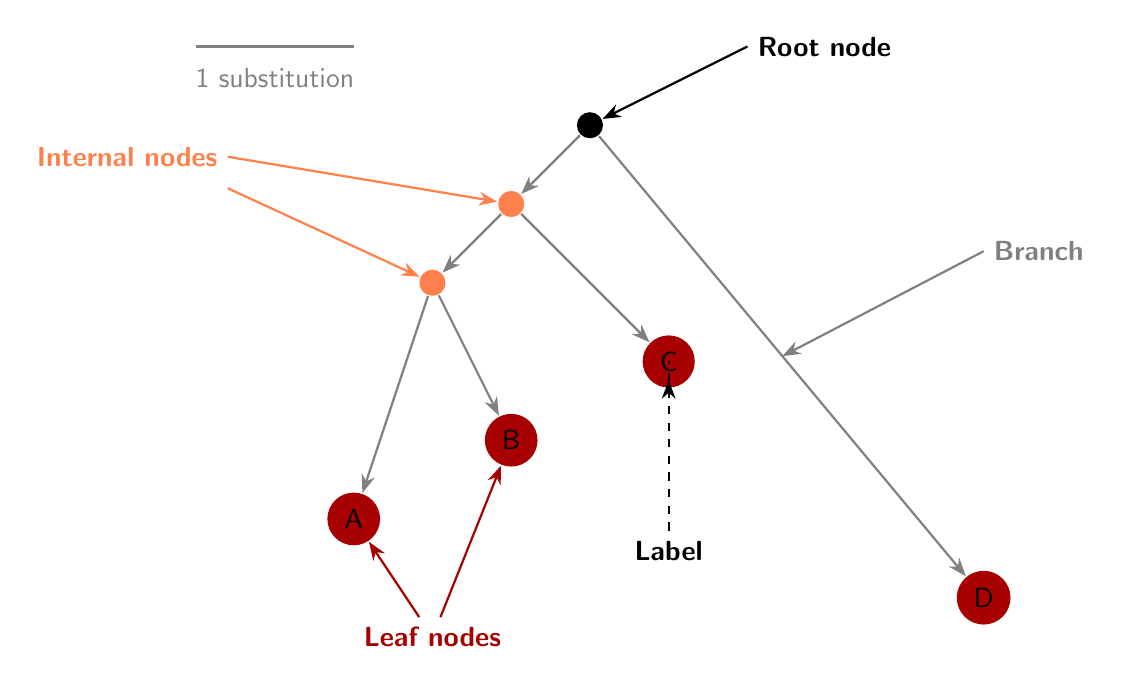
\begin{tikzpicture}[thick, >=Stealth, scale=2]
        % Nodes
        \node[circle, fill=black, label=above:{}] (6) at (1.5, 2) {};
        \node[circle, fill=Peach] (4) at (0.5, 1) {};
        \node[circle, fill=Peach] (5) at (1, 1.5) {};
        \node[circle, fill=Mahogany] (0) at (0, -0.5) {A};
        \node[circle, fill=Mahogany] (2) at (1, 0) {B};
        \node[circle, fill=Mahogany] (1) at (2, 0.5) {C};
        \node[circle, fill=Mahogany] (3) at (4, -1) {D};

        % Directed edges
        \draw[->, gray] (6) -- (5);
        \draw[->, gray] (5) -- (4);
        \draw[->, gray] (6) -- (3) coordinate[midway] (branch1);
        \draw[->, gray] (5) -- (1);
        \draw[->, gray] (4) -- (0);
        \draw[->, gray] (4) -- (2);

        % Annotations
        % Root node
        \draw[->] (2.5, 2.5) node[right]{\textbf{Root node}} -- (6);

        % Internal nodes
        \draw[->, Peach] (-0.8,1.8) node[left]{\textbf{Internal nodes}} -- (5);
        \draw[->, Peach] (-0.8,1.6) -- (4);

        % Leaf nodes
        \node[text=Mahogany] (leaflabel) at (0.5,-1.25) {\textbf{Leaf nodes}};
        \draw[->, Mahogany] (leaflabel) -- (0);
        \draw[->, Mahogany] (leaflabel) -- (2);

        % Label
        \node (clabel) at (2,-0.7) {\textbf{Label}};
        \draw[->, dashed, black] (clabel) -- (1.center) + (0, -0.12);

        % Branches
        \draw[->, gray] (4,1.2) node[right]{\textbf{Branch}} -- (branch1);

        % Scale legend
        \draw[thick, gray] (-1, 2.5) -- ++(1, 0); % a 1-unit horizontal line
        \node[text=gray] at (-0.5, 2.3) {1 substitution};
    \end{tikzpicture}
    \caption{A diagram of a binary, rooted, labelled, non-ultrametric, phylogenetic tree. The Newick representation of this tree is: (((A,B),C),D);.}
    \label{fig:basictree}
\end{figure}

\subsection{Representing trees}

In computer science, traditional ways to represent trees include linked lists or recursive classes, using a node class with attributes for data and references to its children~\cite{knuth1997}. Various methods have been proposed to compress a tree with $n$ leaves into a single-integer representation through counting methods~\cite{rotem1978, proskurowski1980, rohlf1983, palacios2022}. Although such methods allow for a compact representation of trees, they are generally impractical for real-world phylogenetic applications and lack human readability.

In the 1990s, two tree representations were proposed for phylogenetic applications: pair matching~\cite{diaconis1998} and the so-called Newick format (Figure~\ref{fig:basictree})~\cite{olsen1990, felsenstein2004}, the latter of which has since become the \textit{de facto} standard in phylogenetic software. The Newick format represents trees as a set of nested parentheses which enclose pairs of subtrees or pairs of nodes. The main advantages of the Newick format lie in its simplicity and its flexibility, as it can support various annotations such as branch lengths and uncertainty measures. Whilst relatively human-readable for small trees, Newick strings become difficult to visually parse and compare for larger numbers of taxa. Importantly, the Newick format is not \emph{bijective} to the space of (binary) trees, as isomorphisms can be constructed by permuting the order of nodes or subtrees within a pair. In addition, sampling random trees using the Newick format is not intuitively achieved.

A desirable final object to encode trees is a vector, i.e., a one-dimensional array structure. It is one of the most commonly used, flexible, and memory-efficient objects to collect data in many programming languages~\cite{stroustrup2013, harris2020, cormen2022}. A few vector-based representations have been proposed in previous research, including graph polynomials~\cite{liu2021, liu2022}, and the \gls{cblv}~\cite{voznica2022}. However, these formats have not been tailored for tree sampling or phylogenetic inference, as graph polynomials were designed tree clustering and phylogenetic model selection~\cite{liu2021, liu2022}, whereas the \gls{cblv} was implemented for deep learning-based inference of phylogenetic model parameters~\cite{voznica2022}.

\subsection{Phylogenetic inference}
\label{sec:bkg_phylo_inference}

At its core, phylogenetic inference aims at estimating a (binary) phylogenetic tree $T$ for $n$ entities or taxa using comparable data. An intuitive procedure to infer such a tree is to calculate distances between the data at hand. For instance, a naive approach is to build a distance matrix of taxa by comparing the presence/absence of certain characters (or sequences) using a Hamming distance ($d(u,v) = \sum_i 1_{u_i \neq v_i}$). From this distance matrix, methods based on simple agglomerative clustering methods such as \gls{upgma}~\cite{sokal1958} or \gls{nj}~\cite{saitou1987, lefort2015} can be employed to infer a tree. %FastME~\cite{lefort2015} extends \gls{nj} with tree rearrangement operations based on \gls{nni} and \gls{spr} to optimize the \gls{bme} criterion (the best tree is the tree with the shortest total path length)~\cite{pauplin2000}.  \textcolor{red}{parsimony}. 
However, the advent of molecular evolution~\cite{zuckerkandl1965, fitch1967} has propelled the development of new statistical frameworks for phylogenetic inference based on maximum likelihood~\cite{felsenstein1981}, which have become widely accepted as one of the state-of-the-art solutions for phylogenetic inference~\cite{guindon2003, kozlov2019, minh2020}. Central to these methods is Felsteins's likelihood algorithm~\cite{felsenstein1981}, an dynamic programming algorithm to calculate the likelihood of a phylogenetic tree given character data (e.g., nucleotide bases or amino acid residues). Importantly, it leaverages Markov models of substitution to compute the probabilities of changes in these (homologous) characters~\cite{duchene2024}. In DNA, notable substitution models are the naive Jukes-Cantor model~\cite{jukes1969}, which assumes that all substitutions occur with equal probability, and the \gls{gtr} model~\cite{tavare1986}, which allows each type of substitution to have its own rate and accounts for unequal base frequencies. For protein-based analyses, substitution models are often empirically derived from large alignments of homologous proteins. Examples include the WAG~\cite{whelan2001} and LG~\cite{le2008} models.

% In DNA, substitutions are divided into transitions (interchanges of two bases of the same family: A$\leftrightarrow$G for purines, C$\leftrightarrow$T for pyrimidines) and transversions (exchanges between two bases of different families, e.g., A$\leftrightarrow$C). For DNA, the most naive model is the Jukes-Cantor model~\cite{jukes1969}, which assumes that all substitutions are equally likely to happen, e.g., p(A$\rightarrow$G) = p(A$\rightarrow$C) = p(A$\rightarrow$T) = 1/3. More sophisticated models make additional assumptions regarding evolutionary processes, with the \gls{gtr} model~\cite{tavare1986} being the most general. 
% Using these substitution models, the likelihood of a phylogenetic tree can be calculated using Felsenstein's likelihood~\cite{felsenstein1973}, an efficient dynamic programming algorithm to calculate the probabilities of certain states using a post-order traversal. 
Practically, maximum likelihood–based algorithms can be implemented by starting from a sensible initial tree (e.g., using \gls{nj}) and iteratively optimizing it through successive tree rearrangements. These can be very local, such as \gls{nni}, or more extensive, such as \gls{spr}, \gls{tbr}. Popular software for maximum likelihood-based phylogenetics include PhyML~\cite{guindon2003}, IQ-TREE~\cite{minh2020}, and RAxML-NG~\cite{kozlov2019}. Bayesian frameworks also operate with substitution models and Felsenstein's likelihood, but use MCMC: MrBayes~\cite{huelsenbeck2001} and BEAST~\cite{bouckaert2014, baele2025}. \textcolor{red}{Provide better explanation for Bayesian phylo}.

% These methods rely on a likelihood function to be optimized, and Markov models of substitution, which allow to compute the probabilities of different substitutions (i.e., the replacement of a base by another)~\cite{jukes1969, tavare1986}. All modern phylogenetic ML software implement some version of Felsenstein's likelihood~\cite{felsenstein1973}, an efficient dynamic programming algorithm to calculate the probabilities of certain states (e.g, nucleotides or amino acids) using a post-order traversal. 

% Using these substitution models, we can derive a recursive likelihood function for a binary tree. This is called Felsenstein's likelihood~\cite{felsenstein1973}. With these two attributes, we can implement maximum likelihood-based algorithms, starting from a sensible tree (e.g., from neighbour joining) and optimizing the tree by trying tree moves. These can be very local, such as \gls{nni}, or more general, such as \gls{spr}, \gls{tbr}. Popular software include IQ-TREE~\cite{minh2020} and RAxML-NG~\cite{kozlov2019}. Bayesian frameworks also operate with substitution models and Felsenstein's likelihood, but use MCMC: MrBayes~\cite{huelsenbeck2001} and BEAST~\cite{bouckaert2014, baele2025}. \textcolor{red}{Provide better explanation for Bayesian phylo}.

\subsection{Structure-based phylogenetics}

While genes contain genetic information, \emph{proteins} are the primary effectors of that information, acting as catalysts for most cell functions. They consist in one or more chains of amino acids \emph{folded} into a specific three-dimensional structure. The structure is largely pre-determined by the underlying chain of amino acids~\cite{anfinsen1973} and is crucial to the protein's function. From an evolutionary perspective, protein structures are posited to be more conserved~\cite{illergaard2009} than amino acid sequences (which are in turn inherently more conserved than nucleotide sequences due to codon degeneracy). In addition to thermodynamic constraints which sharply limit plausible conformations of a protein, empirical evidence from homologous proteins has shown that structure tends to reflect evolutionary constraints and functional similarities more reliably than raw DNA sequences~\cite{rost1999, illergaard2009, moi2022}. Nevertheless, comparing continuous, three-dimensional, protein structures for phylogenetic analysis is less obvious than discrete, linear sequences. Protein structures are spatial and physicochemical interactions, while sequences are simply linear arrangements of residues (nucleotides or amino acids) that can be directly aligned and compared. A substantial body of research has been dedicated to developing structure comparison metrics for distance-based phylogenetics, such as SSM~\cite{krissinel2004} or TM-Align~\cite{zhang2005}. More recently, the deep learning revolution~\cite{lecun2015} has propelled new avenues for structure-based phylogenetics. On the one hand, embeddings from \glspl{plm} (e.g., ESM~\cite{lin2023, hayes2025}, MSA Transformer~\cite{rao2021}) are shown to encode phylogenetic information~\cite{lupo2022, tule2025}. However, \glspl{plm} are currently of limited precision out of the box due to the coarseness of their training set~\cite{gomez2024}. This makes them impractical for pandemic-related phylogenetics, as analyses usually revolve around comparing variants which only differ by a few mutations~\cite{markov2023}. Another avenue consists in discretizing 3D structures into a finite set of characters, which could be then used downstream for maximum likelihood-based inference. A notable contribution is the \gls{vqvae} model developed within the Foldseek toolkit~\cite{vankempen2024}, whose encoder maps each residue in a strucure to one of 20 discrete characters using geometrical features (e.g., torsion angles between $C_\alpha$ atoms, distances) calculated with its nearest neighbour. Originally developed for protein structure search and clustering, the 3Di model has been used for phylogenetic analyses of diverse protein families (e.g., ferritins~\cite{puente2023}, RRNPPA quorum sensing receptors~\cite{moi2023}, and histones~\cite{fullmer2025}), but this model has, to the best of my knowledge, not yet been leveraged for pathogenic protein phylogenetics.

% genomics, proteomics, phenomics

% Ternary, quarternary structures.

% Structures are posited to be more conserved than sequences~\cite{illergaard2009}. Homologous proteins are more likely to reflect evolutionary constraints and functional similarities than raw DNA sequences.

% Comparing structures is naturally more difficult than sequences; it consists of one or more chains that are folded into complex 3D conformations influenced by spatial and physicochemical interactions, while sequences are simply linear arrangements of residues (nucleotides or amino acids) that can be directly aligned and compared.

% For deep phylogenetics, this can be very cool as very divergent sequences can actually have very similar structures \textcolor{red}{citation needed}

% Original methods for comparing protein structures were distance-based, using methods to "align" protein structures such as TM-align~\cite{zhang2005}. With the advent of new protein structure prediction models such as AlphaFold~\cite{jumper2021, gomez2024, abramson2024}, ColabFold~\cite{mirdita2022}, and ESM~\cite{lin2023, hayes2025}, it would be tempting to i) fold a whole bunch of proteins - this has created lots of large-scale protein atlases~\cite{varadi2022, lin2023, kim2025b} and ii) potentially compare embeddings from these models for downstream phylogenetic analysis. While it has been shown that these models do capture some signal~\cite{lupo2022, tule2025}, as of now these models are of limited precision out of the box when it comes to variants of a same species due to the coarseness of their training set~\cite{gomez2024}.

% In parlallel, other have been made to discretize structures into a sequence of finite states to be able to perform similar maximum-likelihood based methods (see \nameref{sec:bkg_phylo_inference}). These exploit geometrical conformations of $C_\alpha$ atoms and/or their angles. The most popular is 3Di, a learnable discretizer based on a \gls{vqvae} trained on $\approx$ 10,000 protein sequences that maps geometrical angles and distances between $C_\alpha$ atoms to a discrete state. A burgeoning body of literature has worked on the 3di alphabet for various phylogenetic analyses~\cite{moi2023, puente2023}, but none have looked at the pandemic preparedness angle.

% \item Structure-based phylogenetics
% \begin{itemize}
%     \item protein folding
%     \item protein structures: ternary, quaternary etc
%     \item domains
%     \item protein structure prediction
%     \item 3di
% \end{itemize}

\section{Animal welfare for pandemic preparedness}
\label{sec:bkg_animal_welfare}

Most recent pandemics have all been of zoonotic origin~\cite{vora2022}. Although getting increasingly cheaper and accessible, sequencing and protein folding remain poorly scalable when it comes to monitoring animal reservoirs. Something about farming and food security. Current flu epidemic. There is thus a strong demand for tools that could help monitor such reservoirs as well as livestock while minimizing contact with populations. The deep learning revolution~\cite{lecun2015} has catalysed the production of a plethora of methods for the estimation of pose in humans and animals as well as object tracking. This has become very popular in behavioral neuroscience, as these can help put actual numbers and measurements to behavioral experiments~\cite{mathis2018, graving2019, gunel2019, pereira2022, lauer2022}. The most popular is \gls{dlc}~\cite{mathis2018}, which has greatly contributed to making these methods accessible to scientists with little training in computer science. However, their potential for large-scale (i.e, lots of objects) experiments remains relatively unexplored. One interesting case is poultry farming: chickens can carry avian flu, are susceptible to be in contact with tons of wild birds, and they are a super important food source for humans.

\subsection{Video surveillance}

\subsection{Challenges}

\begin{itemize}
\item Animal tracking
\begin{itemize}
    \item deep learning
    \item optical flow
    \item deeplabcut
    \item broilers
    \item pathogens: campylobacter, flu, round worm
    \item video data
\end{itemize}
\end{itemize}

figure: illustration of optical flow

\chapter{Methods}
\section{Study 1: Phylo2Vec}
The initial goal of this study was to derive new analysis frameworks for phylogenetics by representing phylogenetics as something more malleable, e.g., a set of features for machine learning. This led to the development of \gls{p2v} (or Phylo2Vec)~\cite{penn2025, scheidwasser2025}, a representation of phylogenetic tree topologies as integer vectors. Inspired by Yule processes~\cite{steel2001} and tree counting strategies~\cite{knuth1973, rotem1978, proskurowski1980, rohlf1983}, the core idea is to describe \emph{where} leaves are iteratively added within an existing tree topology. The construction of phylo2vec builds upon the work of Rohlf~\cite{rohlf1983} and Dinh~\cite{dinh2010}, but differs in its edge labelling strategy and, in the case of Rohlf~\cite{rohlf1983}, in preserving the tree-construction process within the vector representation. Beyond this conceptual shift, our contributions are fourfold: (i) rigorous proofs that the vector representation is bijective with the space of binary rooted trees~\cite{penn2025}, (ii) an extended matrix format to incorporate branch length information, (iii) empirical evidence of its usability for phylogenetic inference, and (iv) robust and open-source software for manipulating phylogenetic trees using this representation~\cite{scheidwasser2025}.

The simple constraint of the phylo2vec formulation notably allows for rapid tree sampling, efficient compression, and straightforward comparison of tree topologies. In addition, the simplicity of such a vector format makes it a convenient starting object for phylogenetic tree manipulation, which is showcased in the \texttt{phylo2vec} software package~\cite{scheidwasser2025}. The package also highlights potential avenues for phylo2vec-based phylogenetic inference, including non-traditional optimisation approaches such as (gradient-based \gls{bme} (GradME)~\cite{penn2023}.

\subsection{Definitions}
\label{p2v:definitions}
\emph{Phylo2Vec} denotes a bijective mapping from phylogenetic tree topologies to constrained integer vectors. It relies on the following assumptions regarding tree topology construction:

\begin{itemize}[nosep]
    \item Let $T$ be a binary, rooted, phylogenetic tree with $n \geq 2$ leaves and topology $\tau$.
    \item Each leaf is assigned a unique label $\ell \in \{0, \ldots, n-1\}$.
    \item Each internal node is assigned a unique label $\ell' \in \{n, \ldots, 2(n-1)\}$. For each node, the assignment generally depends on its height and descending leaves (see Section~\ref{methods:v2newick}). The root node is always labelled $2(n-1)$.
    \item Each branch (or edge) is labelled according to its target node (i.e., a branch leading to node $\nu$ is labelled $\nu$).
\end{itemize}
\begin{figure}[htbp]
    \centering
    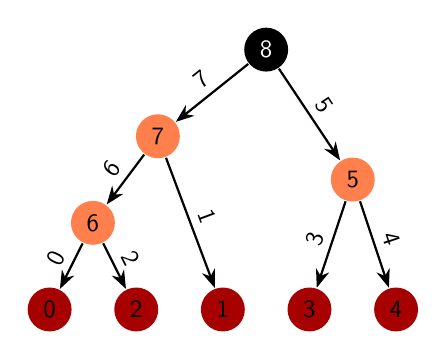
\begin{tikzpicture}[thick, >=Stealth, scale=1.1, every node/.style={scale=0.9}]
        % Nodes
        \node[circle, fill=black, text=white] (8) at (2.5, 3) {8};
        \node[circle, fill=Peach] (7) at (1.25, 2) {7};
        \node[circle, fill=Peach] (6) at (0.5, 1) {6};
        \node[circle, fill=Peach] (5) at (3.5, 1.5) {5};
        \node[circle, fill=Mahogany] (0) at (0, 0) {0};
        \node[circle, fill=Mahogany] (2) at (1, 0) {2};
        \node[circle, fill=Mahogany] (1) at (2, 0) {1};
        \node[circle, fill=Mahogany] (3) at (3, 0) {3};f
        \node[circle, fill=Mahogany] (4) at (4, 0) {4};

        % Directed edges
        \draw[->] (8) -- (5) node[midway, sloped, above] {5};
        \draw[->] (8) -- (7) node[midway, sloped, above] {7};
        \draw[->] (7) -- (1) node[midway, sloped, above] {1};
        \draw[->] (7) -- (6) node[midway, sloped, above] {6};
        \draw[->] (6) -- (0) node[midway, sloped, above] {0};
        \draw[->] (6) -- (2) node[midway, sloped, above] {2};
        \draw[->] (5) -- (4) node[midway, sloped, above] {4};
        \draw[->] (5) -- (3) node[midway, sloped, above] {3};
    \end{tikzpicture}
    \caption{A diagram of a tree topology satisfying phylo2vec assumptions. The vector representation of this tree is $\begin{pmatrix} 0 & 0 & 4 & 3 \end{pmatrix}$ (see Section~\ref{methods:v2newick}).}
    \label{fig:p2vtree}
\end{figure}

Fig.~\ref{fig:p2vtree} depicts an example tree which satisfies these assumptions. Consequently, for any $n$-leaf tree topology, we define an integer vector $\boldsymbol{v}$ of length $n-1$:

\begin{equation}
    \forall n \geq 2 \quad \forall j \in \{0, \ldots, n-2\} \quad v_j \in \{0, \ldots, 2j\}
    \label{eq:p2v}
\end{equation}

We call $\mathbb{V}$ the set of vectors that satisfies Eq.~\ref{eq:p2v}. In this formulation, \textsb{$v_j$ denotes the \emph{edge} from which leaf $j + 1$ descends from} (when added to a tree with $j$ leaves). An immediate property arises from Eq.~\ref{eq:p2v}: the cardinality of the phylo2vec vector set equals that of the set of binary rooted trees~\cite{cavallisforza1967}. Noting $\mathbb{V}_n$ and $\mathbb{T}_n$ as, respectively, the set of vectors and binary trees with $n$ leaves:

\begin{equation}
    |\mathbb{V}_n| = \prod_{j=0}^{n-2}(2j+1) = 1\cdot3\cdot\ldots\cdot2n-3=(2n-3)!! = |\mathbb{T}_n|
    \label{eq:p2v_cardinality}
\end{equation}

Given Eq.~\ref{eq:p2v_cardinality}, showing that there exists an injection from $\mathbb{V}_n$ to $\mathbb{T}_n$ for any $n \geq 2$ is sufficient to demonstrate bijectivity between the two sets. A proof is provided in Penn \textit{et al.}~\cite{penn2025} (see~\ref{appendix:articles}).

A phylo2vec vector is said to be \textit{ordered} if it satisfies:

\begin{equation}
    \forall n \geq 2 \quad \forall j \in \{0, \ldots, n-2\} \quad v_j \in \{0, \ldots, j\}  
    \label{eq:p2v_ordered}
\end{equation}

The term \textit{ordered} refers to the fact that any leaf $i$ will, in a similar vein to Yule processes, descend from an ``older" leaf $j < i$. The cardinality of ordered trees is $\prod_{j=0}^{n-2}(j+1) = (n-1)!$. Whilst a subset of all phylo2vec vectors, ordered trees are more algorithmically efficient to manipulate (see Sections~\ref{methods:v2newick} and~\ref{methods:newick2v}) and more practical for certain downstream phylogenetic applications~\cite{penn2023, penn2025}. Importantly, the \emph{Queue Shuffle} trick~\cite{penn2023} enables the transformation of any \emph{unordered} vector $\boldsymbol{v}$ into an ordered vector.

Conversely, a phylo2vec vector is said to be \textit{completely unordered} if:

\begin{equation}
    \forall n \geq 2 \quad \forall j \in \{0, \ldots, n-2\} \quad v_j \in \{j+1, \ldots, 2j\}  
    \label{eq:p2v_completelyunordered}
\end{equation}

In other words, whereas leaves from an ordered vector descend from leaf branches, leaves from a completely unordered vector all descend from internal branches.

\subsection{Unpacking a vector as a tree}
\label{methods:v2newick}

Unpacking a vector satisfying the phylo2vec conditions in Eq. ~\ref{eq:p2v} is performed by reading the vector from left to right, where one new leaf is added per vector element. Fig.~\ref{fig:v2newick} shows a detailed example of the conversion process. We start from a two-leaf tree with leaves labelled $0$ and $1$ and a root labelled $2$. Following the assumptions in Section~\ref{p2v:definitions}, we label each edge according to its target node. We also add an \emph{extra root} labelled $R$, for which we draw a directed edge from $R$ to $2$. Following the definition of $v_j$ (see Section~\ref{p2v:definitions}), this additional edge is necessary to ensure that all possible $3$ leaf placements are represented from the starting tree (and, by induction, to ensure that all possible $2n-1$ leaf placements can be represented from an $n$-leaf tree~\cite{cavallisforza1967}). From this augmented two-leaf tree, we successively add leaves according to the values of \v, where an iteration $j$ corresponds to adding leaf $j+1$ from branch $v_j$. Importantly, adding a new leaf requires updating the labels of the internal nodes and edges. The general update rule is that the next internal node to be labelled is the parent of the cherry with the highest label. An illustration of this rule is shown in Fig.~\ref{fig:relabelling}.

\begin{figure}[htbp]
    \centering
    \small
    \begin{tabular}{p{2cm} l p{2cm} c c}
    \toprule
    & \v & \textbf{Tree action} & \textbf{Tree action (illustrated)} & \textbf{Tree} \\
    \midrule
    Initial state & \v~= $\begin{pmatrix} 0 \end{pmatrix}$ & - & - & \adjustbox{valign=t}{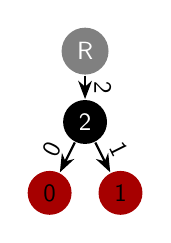
\begin{tikzpicture}[thick, >=Stealth, scale=0.9, every node/.style={scale=0.9}]
        % Nodes
        \node[circle, fill=gray, text=white] (R) at (0.5, 2) {R};
        \node[circle, fill=black, text=white] (2) at (0.5, 1) {2};
        \node[circle, fill=Mahogany] (0) at (0, 0) {0};
        \node[circle, fill=Mahogany] (1) at (1, 0) {1};

        % Directed edges
        \draw[->] (R) -- (2) node[midway, sloped, above] {2};
        \draw[->] (2) -- (1) node[midway, sloped, above] {1};
        \draw[->] (2) -- (0) node[midway, sloped, above] {0};
    \end{tikzpicture}} \\
    Step 1: $v_1 = 0$ \newline Next leaf: 2 & \v~$ = \begin{pmatrix} 0 & 0 \end{pmatrix}$ & Add leaf $2$ from branch 0
    & \adjustbox{valign=t}{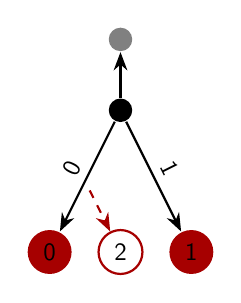
\begin{tikzpicture}[thick, >=Stealth, scale=0.9, every node/.style={scale=0.9}]
        % Nodes
        \node[circle, fill=gray, text=white] (R) at (1, 3) {};
        \node[circle, fill=black, text=white] (2) at (1, 2) {};
        \node[circle, fill=Mahogany] (0) at (0, 0) {0};
        \node[circle, fill=Mahogany] (1) at (2, 0) {1};
        \node[circle, draw=Mahogany] (2leaf) at (1, 0) {2};

        \node (M) at (0.5, 1) {};

        % Directed edges
        \draw[->] (2) -- (R) node[midway, sloped, above] {};
        \draw[->] (2) -- (1) node[midway, sloped, above] {1};
        \draw[->] (2) -- (0) node[midway, sloped, above] {0};
        \draw[->, dashed, text=Mahogany, Mahogany] (M) -- (2leaf) node[midway, sloped, above] {};
    \end{tikzpicture}}
    & \adjustbox{valign=t}{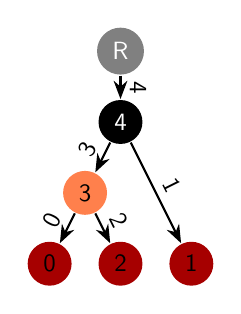
\begin{tikzpicture}[thick, >=Stealth, scale=0.9, every node/.style={scale=0.9}]
        % Nodes
        \node[circle, fill=gray, text=white] (R) at (1, 3) {R};
        \node[circle, fill=black, text=white] (4) at (1, 2) {4};
        \node[circle, fill=Peach] (3) at (0.5, 1) {3};
        \node[circle, fill=Mahogany] (0) at (0, 0) {0};
        \node[circle, fill=Mahogany] (2) at (1, 0) {2};
        \node[circle, fill=Mahogany] (1) at (2, 0) {1};

        % Directed edges
        \draw[->] (R) -- (4) node[midway, sloped, above] {4};
        \draw[->] (4) -- (3) node[midway, sloped, above] {3};
        \draw[->] (4) -- (1) node[midway, sloped, above] {1};
        \draw[->] (3) -- (2) node[midway, sloped, above] {2};
        \draw[->] (3) -- (0) node[midway, sloped, above] {0};
    \end{tikzpicture}} \\
    Step 2: $v_2 = 4$ \newline Next leaf: 3 & \v~$ = \begin{pmatrix} 0 & 0 & 4 \end{pmatrix}$ & Add leaf $3$ from branch 4 & 
    \adjustbox{valign=t}{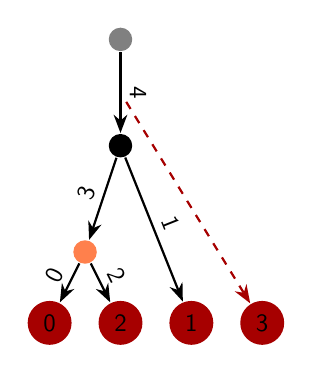
\begin{tikzpicture}[thick, >=Stealth, scale=0.9, every node/.style={scale=0.9}]
        % Nodes
        \node[circle, fill=gray, text=white] (R) at (1, 4) {};
        \node[circle, fill=black, text=white] (4) at (1, 2.5) {};
        \node[circle, fill=Peach] (3) at (0.5, 1) {};
        \node[circle, fill=Mahogany] (0) at (0, 0) {0};
        \node[circle, fill=Mahogany] (2) at (1, 0) {2};
        \node[circle, fill=Mahogany] (1) at (2, 0) {1};
        \node[circle, fill=Mahogany] (3leaf) at (3, 0) {3};

        \node (M) at (1, 3.25) {};

        % Directed edges
        \draw[->] (R) -- (4) node[midway, sloped, above] {4};
        \draw[->] (4) -- (3) node[midway, sloped, above] {3};
        \draw[->] (4) -- (1) node[midway, sloped, above] {1};
        \draw[->] (3) -- (2) node[midway, sloped, above] {2};
        \draw[->] (3) -- (0) node[midway, sloped, above] {0};
        \draw[->, dashed, Mahogany] (M) -- (3leaf) node[midway, sloped, above] {};
    \end{tikzpicture}} & 
    \adjustbox{valign=t}{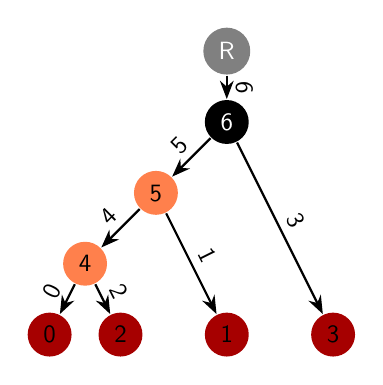
\begin{tikzpicture}[thick, >=Stealth, scale=0.9, every node/.style={scale=0.9}]
        % Nodes
        \node[circle, fill=gray, text=white] (R) at (2.5, 4) {R};
        \node[circle, fill=black, text=white] (6) at (2.5, 3) {6};
        \node[circle, fill=Peach] (5) at (1.5, 2) {5};
        \node[circle, fill=Peach] (4) at (0.5, 1) {4};
        \node[circle, fill=Mahogany] (0) at (0, 0) {0};
        \node[circle, fill=Mahogany] (2) at (1, 0) {2};
        \node[circle, fill=Mahogany] (1) at (2.5, 0) {1};
        \node[circle, fill=Mahogany] (3) at (4, 0) {3};

        % Directed edges
        \draw[->] (R) -- (6) node[midway, sloped, above] {6};
        \draw[->] (6) -- (3) node[midway, sloped, above] {3};
        \draw[->] (6) -- (5) node[midway, sloped, above] {5};
        \draw[->] (5) -- (4) node[midway, sloped, above] {4};
        \draw[->] (5) -- (1) node[midway, sloped, above] {1};
        \draw[->] (4) -- (2) node[midway, sloped, above] {2};
        \draw[->] (4) -- (0) node[midway, sloped, above] {0};
    \end{tikzpicture}} \\
    Step 3: $v_3 = 3$ \newline Next leaf: 4 & \v~$ = \begin{pmatrix} 0 & 0 & 4 & 3 \end{pmatrix}$ & Add leaf 4 from branch 3 \newline Remove the extra root (last step) & 
    \adjustbox{valign=t}{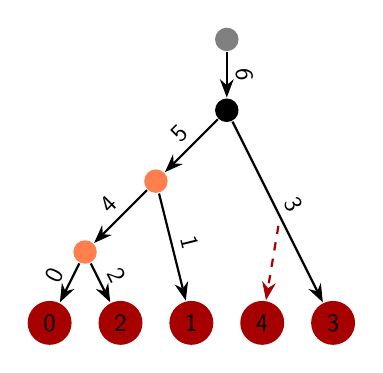
\begin{tikzpicture}[thick, >=Stealth, scale=0.9, every node/.style={scale=0.9}]
        % Nodes
        \node[circle, fill=gray, text=white] (R) at (2.5, 4) {};
        \node[circle, fill=black, text=white] (6) at (2.5, 3) {};
        \node[circle, fill=Peach] (5) at (1.5, 2) {};
        \node[circle, fill=Peach] (4) at (0.5, 1) {};
        \node[circle, fill=Mahogany] (0) at (0, 0) {0};
        \node[circle, fill=Mahogany] (2) at (1, 0) {2};
        \node[circle, fill=Mahogany] (1) at (2, 0) {1};
        \node[circle, fill=Mahogany] (3) at (4, 0) {3};
        \node[circle, fill=Mahogany] (4leaf) at (3, 0) {4};

        \node (M) at (3.25, 1.5) {};

        % Directed edges
        \draw[->] (R) -- (6) node[midway, sloped, above] {6};
        \draw[->] (6) -- (3) node[midway, sloped, above] {3};
        \draw[->] (6) -- (5) node[midway, sloped, above] {5};
        \draw[->] (5) -- (4) node[midway, sloped, above] {4};
        \draw[->] (5) -- (1) node[midway, sloped, above] {1};
        \draw[->] (4) -- (2) node[midway, sloped, above] {2};
        \draw[->] (4) -- (0) node[midway, sloped, above] {0};
        \draw[->, dashed, Mahogany] (M) -- (4leaf) node[midway, sloped, above] {};
    \end{tikzpicture}} & 
    \adjustbox{valign=t}{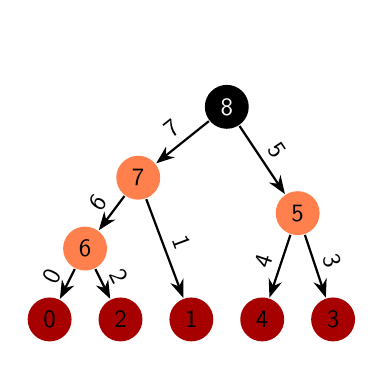
\begin{tikzpicture}[thick, >=Stealth, scale=0.9, every node/.style={scale=0.9}]
        % Nodes
        \node (R) at (2.5, 4) {};
        \node[circle, fill=black, text=white] (8) at (2.5, 3) {8};
        \node[circle, fill=Peach] (7) at (1.25, 2) {7};
        \node[circle, fill=Peach] (6) at (0.5, 1) {6};
        \node[circle, fill=Peach] (5) at (3.5, 1.5) {5};
        \node[circle, fill=Mahogany] (0) at (0, 0) {0};
        \node[circle, fill=Mahogany] (2) at (1, 0) {2};
        \node[circle, fill=Mahogany] (1) at (2, 0) {1};
        \node[circle, fill=Mahogany] (3) at (4, 0) {3};
        \node[circle, fill=Mahogany] (4) at (3, 0) {4};

        % Directed edges
        \draw[->] (8) -- (5) node[midway, sloped, above] {5};
        \draw[->] (8) -- (7) node[midway, sloped, above] {7};
        \draw[->] (7) -- (1) node[midway, sloped, above] {1};
        \draw[->] (7) -- (6) node[midway, sloped, above] {6};
        \draw[->] (6) -- (0) node[midway, sloped, above] {0};
        \draw[->] (6) -- (2) node[midway, sloped, above] {2};
        \draw[->] (5) -- (4) node[midway, sloped, above] {4};
        \draw[->] (5) -- (3) node[midway, sloped, above] {3};
    \end{tikzpicture}} \\
    \bottomrule
    \end{tabular}
    \caption{Unpacking \v~$ = \begin{pmatrix} 0 & 0 & 4 & 3 \end{pmatrix}$ graphically as a tree. Adapted from Penn \textit{et al.}~\cite{penn2025}.}
    \label{fig:v2newick}
\end{figure}

\clearpage

\begin{figure}
    \centering
    \small
    \begin{tabular}{p{4cm} p{4cm} c}
    \toprule
    \textsb{State} & \textsb{Action} & \textsb{Tree} \\
    \midrule
    Initial state \newline Added leaf 4 from branch 3 & Discard current internal node \& branch labels  & \adjustbox{valign=t}{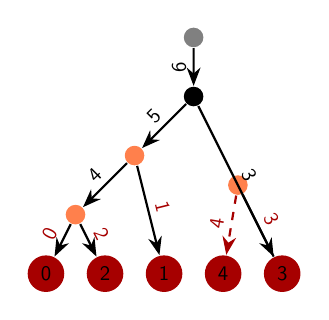
\begin{tikzpicture}[thick, >=Stealth, scale=0.75, every node/.style={scale=0.75}]
        % Nodes
        \node[circle, fill=gray, text=white] (R) at (2.5, 4) {};
        \node[circle, fill=black, text=white] (6) at (2.5, 3) {};
        \node[circle, fill=Peach] (5) at (1.5, 2) {};
        \node[circle, fill=Peach] (4) at (0.5, 1) {};
        \node[circle, fill=Mahogany] (0) at (0, 0) {0};
        \node[circle, fill=Mahogany] (2) at (1, 0) {2};
        \node[circle, fill=Mahogany] (1) at (2, 0) {1};
        \node[circle, fill=Mahogany] (3) at (4, 0) {3};
        \node[circle, fill=Mahogany] (4leaf) at (3, 0) {4};

        \node[circle, fill=Peach] (M) at (3.25, 1.5) {};

        % Directed edges
        \draw[->] (R) -- (6) node[midway, sloped, above] {\st{6}};
        \draw[->] (6) -- (3) node[midway, sloped, above] {\st{3}};
        \draw[->] (6) -- (5) node[midway, sloped, above] {\st{5}};
        \draw[->] (5) -- (4) node[midway, sloped, above] {\st{4}};
        \draw[->, text=Mahogany] (5) -- (1) node[midway, sloped, above] {1};
        \draw[->, text=Mahogany] (4) -- (2) node[midway, sloped, above] {2};
        \draw[->, text=Mahogany] (4) -- (0) node[midway, sloped, above] {0};
        \draw[->, dashed, Mahogany, text=Mahogany] (M) -- (4leaf) node[midway, sloped, above] {4};
        \draw[text=Mahogany] (M) -- (3) node[midway, sloped, above] {3};
    \end{tikzpicture}} \\
    2 cherries: (0,2), (3,4) \newline Next parent = 5 & $\max(0, 2, 3, 4) = 4$ \newline Label the parent of 4 as 5 \newline Prune leaf \textsb{4} & \adjustbox{valign=t}{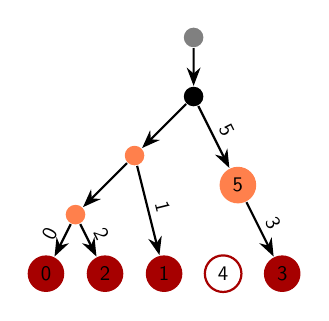
\begin{tikzpicture}[thick, >=Stealth, scale=0.75, every node/.style={scale=0.75}]
        % Nodes
        \node[circle, fill=gray, text=white] (R) at (2.5, 4) {};
        \node[circle, fill=black, text=white] (6) at (2.5, 3) {};
        \node[circle, fill=Peach] (5) at (1.5, 2) {};
        \node[circle, fill=Peach] (4) at (0.5, 1) {};
        \node[circle, fill=Mahogany] (0) at (0, 0) {0};
        \node[circle, fill=Mahogany] (2) at (1, 0) {2};
        \node[circle, fill=Mahogany] (1) at (2, 0) {1};
        \node[circle, fill=Mahogany] (3) at (4, 0) {3};
        \node[circle, draw=Mahogany] (4leaf) at (3, 0) {4};

        \node[circle, fill=Peach] (M) at (3.25, 1.5) {5};

        % Directed edges
        \draw[->] (R) -- (6) node[midway, sloped, above] {};
        \draw[->] (6) -- (M) node[midway, sloped, above] {5};
        \draw[->] (6) -- (5) node[midway, sloped, above] {};
        \draw[->] (5) -- (4) node[midway, sloped, above] {};
        \draw[->] (5) -- (1) node[midway, sloped, above] {1};
        \draw[->] (4) -- (2) node[midway, sloped, above] {2};
        \draw[->] (4) -- (0) node[midway, sloped, above] {0};
        \draw[->] (M) -- (3) node[midway, sloped, above] {3};
    \end{tikzpicture}} \\
    1 cherry: (0,2) \newline Next parent = 6 & $\max(0, 2) = 2$ \newline Label the parent of 2 as 6 \newline Prune leaf \textsb{2} & \adjustbox{valign=t}{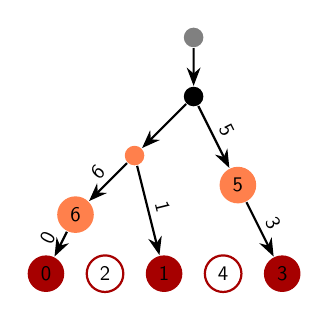
\begin{tikzpicture}[thick, >=Stealth, scale=0.75, every node/.style={scale=0.75}]
        % Nodes
        \node[circle, fill=gray, text=white] (R) at (2.5, 4) {};
        \node[circle, fill=black, text=white] (6) at (2.5, 3) {};
        \node[circle, fill=Peach] (5) at (1.5, 2) {};
        \node[circle, fill=Peach] (4) at (0.5, 1) {6};
        \node[circle, fill=Mahogany] (0) at (0, 0) {0};
        \node[circle, draw=Mahogany] (2) at (1, 0) {2};
        \node[circle, fill=Mahogany] (1) at (2, 0) {1};
        \node[circle, fill=Mahogany] (3) at (4, 0) {3};
        \node[circle, draw=Mahogany] (4leaf) at (3, 0) {4};

        \node[circle, fill=Peach] (M) at (3.25, 1.5) {5};

        % Directed edges
        \draw[->] (R) -- (6) node[midway, sloped, above] {};
        \draw[->] (6) -- (M) node[midway, sloped, above] {5};
        \draw[->] (6) -- (5) node[midway, sloped, above] {};
        \draw[->] (5) -- (4) node[midway, sloped, above] {6};
        \draw[->] (5) -- (1) node[midway, sloped, above] {1};
        \draw[->] (4) -- (0) node[midway, sloped, above] {0};
        \draw[->] (M) -- (3) node[midway, sloped, above] {3};
    \end{tikzpicture}} \\
    1 cherry: (0,1) \newline Next parent = 7 & $\max(0, 1) = 1$ \newline Label the parent of 1 as 7 \newline Prune leaf \textsb{1} & \adjustbox{valign=t}{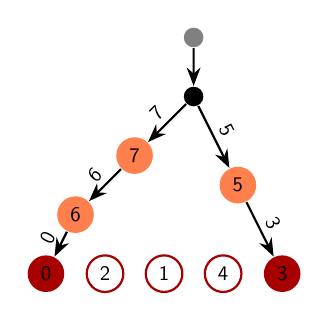
\begin{tikzpicture}[thick, >=Stealth, scale=0.75, every node/.style={scale=0.75}]
        % Nodes
        \node[circle, fill=gray, text=white] (R) at (2.5, 4) {};
        \node[circle, fill=black, text=white] (6) at (2.5, 3) {};
        \node[circle, fill=Peach] (5) at (1.5, 2) {7};
        \node[circle, fill=Peach] (4) at (0.5, 1) {6};
        \node[circle, fill=Mahogany] (0) at (0, 0) {0};
        \node[circle, draw=Mahogany] (2) at (1, 0) {2};
        \node[circle, draw=Mahogany] (1) at (2, 0) {1};
        \node[circle, fill=Mahogany] (3) at (4, 0) {3};
        \node[circle, draw=Mahogany] (4leaf) at (3, 0) {4};

        \node[circle, fill=Peach] (M) at (3.25, 1.5) {5};

        % Directed edges
        \draw[->] (R) -- (6) node[midway, sloped, above] {};
        \draw[->] (6) -- (M) node[midway, sloped, above] {5};
        \draw[->] (6) -- (5) node[midway, sloped, above] {7};
        \draw[->] (5) -- (4) node[midway, sloped, above] {6};
        \draw[->] (4) -- (0) node[midway, sloped, above] {0};
        \draw[->] (M) -- (3) node[midway, sloped, above] {3};
    \end{tikzpicture}} \\
    1 cherry: (0,3) \newline Next parent = 8 & $\max(0, 3) = 3$ \newline Label the parent of 1 as 8 \newline Prune leaf \textsb{3} & \adjustbox{valign=t}{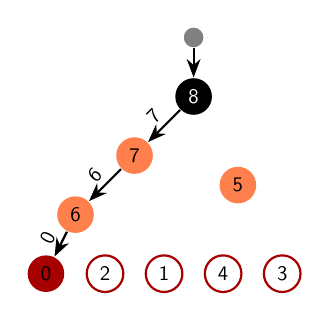
\begin{tikzpicture}[thick, >=Stealth, scale=0.75, every node/.style={scale=0.75}]
        % Nodes
        \node[circle, fill=gray, text=white] (R) at (2.5, 4) {};
        \node[circle, fill=black, text=white] (6) at (2.5, 3) {8};
        \node[circle, fill=Peach] (5) at (1.5, 2) {7};
        \node[circle, fill=Peach] (4) at (0.5, 1) {6};
        \node[circle, fill=Mahogany] (0) at (0, 0) {0};
        \node[circle, draw=Mahogany] (2) at (1, 0) {2};
        \node[circle, draw=Mahogany] (1) at (2, 0) {1};
        \node[circle, draw=Mahogany] (3) at (4, 0) {3};
        \node[circle, draw=Mahogany] (4leaf) at (3, 0) {4};

        \node[circle, fill=Peach] (M) at (3.25, 1.5) {5};

        % Directed edges
        \draw[->] (R) -- (6) node[midway, sloped, above] {};
        % \draw[->] (6) -- (M) node[midway, sloped, above] {5};
        \draw[->] (6) -- (5) node[midway, sloped, above] {7};
        \draw[->] (5) -- (4) node[midway, sloped, above] {6};
        \draw[->] (4) -- (0) node[midway, sloped, above] {0};
        % \draw[->] (M) -- (3) node[midway, sloped, above] {3};
    \end{tikzpicture}} \\
    \bottomrule
    \end{tabular}
    \caption{A visual algorithm for re-labelling internal nodes after adding a new leaf. Example with Step 3 of Fig.~\ref{fig:v2newick} for \v~$ = \begin{pmatrix} 0 & 0 & 4 & 3 \end{pmatrix}$. Adapted from Penn \textit{et al.}~\cite{penn2025}.}
    \label{fig:relabelling}
\end{figure}

In practice, unpacking a vector in Newick format requires two steps in the current version of the \texttt{phylo2vec} package~\cite{scheidwasser2025}. First, we build a list of leaf pairs which describe a post-order traversal of the tree (Algorithm~\ref{alg:to_pairs}; see Fig.~\ref{fig:to_pairs} for an example). The pair $(c_1, c_2)$ indicates that $c_2$ is added such that it forms a cherry with $c_1$. For ordered vectors (see Eq.~\ref{eq:p2v_ordered}), the vector immediately translates into an ordered traversal as new leaves are added from leaf branches (i.e., extant branches). For completely unordered vectors (see Eq.~\ref{eq:p2v_completelyunordered}), insert operations are needed to preserve the post-order nature of the list of pairs, with the insert position depending on $v_j$ and $j$. From this list of pairs, we can form a Newick representation of the tree by iteratively merging Newick substrings initiated from the leaf pair list (see Fig.~\ref{fig:build_newick} for an example).

\begin{algorithm}[htbp]
\begin{algorithmic}[1]
\Require \v $\in \mathbb{V}$ of length $n-1$ with $n$ the number of leaves
\State \textbf{Initialize} $\bm{p} \gets [(0, 1)]$ \Comment{Cherry list for a starting 2-leaf tree}
\For{$j \gets 1$ \textbf{to} $n - 2$}
    \State $\ell \gets i + 1$ \Comment next leaf
    \If{$v_j \leq j$} 
        \Comment{``Ordered" node: $\ell$ arises from a leaf branch. Append is sufficient}
        \State $\bm{p}.\text{append}\big((v_j, \ell)\big)$
    \Else
        \Comment{``Unordered" node: $\ell$ arises from an internal branch}.
        \State $\hat{j} \gets 2j - v_j$ \Comment{Insertion position}
        \State $c_1 \gets \bm{p}_{\hat{j}, 0}$ \Comment{Smallest descending leaf of that branch}
        \State $\bm{p}.\text{insert}\big(\hat{j}, (c_1, \ell)\big)$
    \EndIf
\EndFor
\State \Return $\bm{p}$
\end{algorithmic}
\caption{Naive implementation of a post-order traversal formation from a phylo2vec vector \v.}
\label{alg:to_pairs}
\end{algorithm}
\begin{figure}[htbp]
    \centering
    \small
    \begin{tabular}{p{2cm} l p{5cm} c}
    \toprule
    Step ($j$) & \v & \textbf{Action} & $\bm{p}$ \\
    \midrule
    Step 0 \newline Initial state & \v~= $\begin{pmatrix} 0 \end{pmatrix}$ & - & $\begin{pmatrix}
        0 & 1
    \end{pmatrix}$ \\~\\
    Step 1: $v_1 = \RoyalBlue{0}$ \newline Next leaf: \Mahogany{2} & \v~ = $\begin{pmatrix} 0 & 0\end{pmatrix}$ & $v_j \leq j$ \newline \Mahogany{2} forms a cherry with \textcolor{Violet}{0} \newline \textbf{append (\textcolor{Violet}{0}, \Mahogany{2})} & \adjustbox{valign=t}{$\begin{pmatrix}
        0 & 1 \\
        \textcolor{Violet}{0} & \Mahogany{2}
    \end{pmatrix}$} \\~\\
    Step 2: $v_2 = \RoyalBlue{4}$ \newline Next leaf: \Mahogany{3} & \v~ = $\begin{pmatrix} 0 & 0 & 4 \end{pmatrix}$ & $v_j > j$ \newline smallest descendant of branch \RoyalBlue{4} is \textcolor{Violet}{0} (see~\ref{fig:p2vtree}) \newline \Mahogany{3} thus formed a cherry with \textcolor{Violet}{0} \newline \textbf{insert (\textcolor{Violet}{0}, \Mahogany{3}) at index $\textcolor{RoyalBlue}{4} - 2j = 0$} & \adjustbox{valign=t}{$\begin{pmatrix}
        \textcolor{Violet}{0} & \Mahogany{3} \\
        0 & 1 \\
        0 & 2
    \end{pmatrix}$} \\~\\
    Step 3: $v_3 = \RoyalBlue{3}$ \newline Next leaf: \Mahogany{4} & \v~ = $\begin{pmatrix} 0 & 0 & 4 & 3 \end{pmatrix}$ & $v_j \leq j$ \newline \Mahogany{4} forms a cherry with \textcolor{Violet}{3} \newline \textbf{append (\textcolor{Violet}{3}, \Mahogany{4})}  & \adjustbox{valign=t}{$\begin{pmatrix}
        0 & 3 \\
        0 & 1 \\
        0 & 2 \\
        \textcolor{Violet}{3} & \Mahogany{4}
    \end{pmatrix}$} \\
    \bottomrule
    \end{tabular}
    \caption{Illustration of Algorithm~\ref{alg:to_pairs} using \v~ = $\begin{pmatrix} 0 & 0 & 4 & 3 \end{pmatrix}$ as an example. The algorithm aims at building a list of ``cherries" ordered in a post-order fashion from \v.}
    \label{fig:to_pairs}
\end{figure}

\begin{figure}[htbp]
    \centering
    \begin{tabular}{p{6cm}l}
        \toprule
        Initial state: cherry list & $\bm{p} = \begin{pmatrix}
            \textcolor{RubineRed}{0} & 3 \\
            \textcolor{RubineRed}{0} & 1 \\
            \textcolor{RubineRed}{0} & 2 \\
            \textcolor{Purple}{3} & 4 \\
        \end{pmatrix}$ \\
        \midrule
        Stage 1: build a string cache \newline for each label $\ell$, prepend \texttt{(} each time it appears as a left child in $\bm{p}$ & $\kappa = 
        \begin{Bmatrix} 
        \text{leaf} & \text{sub-string} \\
        0 & \texttt{`\textcolor{RubineRed}{(((}0'} \\ 
        1 & \texttt{`1'} \\ 
        2 & \texttt{`2'} \\ 
        3 & \texttt{`\textcolor{Purple}{(}3'} \\ 
        4 & \texttt{`4'} \end{Bmatrix}$ 
        \\
        \midrule
        Stage 2: process $\bm{p}$ from bottom to top \\
        \quad Step 1: (3, 4), next parent = 5 \newline\hspace*{1em}Pair \textcolor{Mahogany}{4} with \textcolor{Purple}{3}, append \textcolor{RoyalBlue}{5} & $\kappa =
        \begin{Bmatrix} 0 & \texttt{`(((0'} \\ 
        1 & \texttt{`1'} \\ 
        2 & \texttt{`2'} 
        \\ 3 & 
        \texttt{`\textcolor{Purple}{(3},\textcolor{Mahogany}{4})\textcolor{RoyalBlue}{5}'} 
        \end{Bmatrix}$ \\~\\
        \quad Step 2: (0, 2), next parent = 6 \newline\hspace*{1em}Pair \textcolor{Mahogany}{2} with \textcolor{Purple}{0}, append \textcolor{RoyalBlue}{6} & $\kappa =
        \begin{Bmatrix} 
            0 & \texttt{`\textcolor{Purple}{(((0},\textcolor{Mahogany}{2})\textcolor{RoyalBlue}{6}'} \\ 
            1 & \texttt{`1'} \\ 3 & \texttt{`(3,4)5'} 
        \end{Bmatrix}$ \\~\\
        \quad Step 3: (0, 1), next parent = \textcolor{RoyalBlue}{7} \newline\hspace*{1em}Pair \textcolor{Mahogany}{1} with 0, append \textcolor{RoyalBlue}{7} & $\kappa =
        \begin{Bmatrix} 
        0 & \texttt{`\textcolor{Purple}{(((0,2)6},\textcolor{Mahogany}{1})\textcolor{RoyalBlue}{7}'} 
        \\ 3 & \texttt{`(3,4)5'}
        \end{Bmatrix}$ \\~\\
        \quad Step 4: (0, 3), next parent = 8 \newline\hspace*{1em}Pair \textcolor{Mahogany}{3} with 0, append \textcolor{RoyalBlue}{8} & $\kappa =
        \begin{Bmatrix} 
        0 & \texttt{`\textcolor{Purple}{(((0,2)6,1)7},\textcolor{Mahogany}{(3,4)5})\textcolor{RoyalBlue}{8}'} 
        \end{Bmatrix}$ \\
        \midrule
        Output: Append \texttt{;} to $\kappa_0$ & \texttt{\textbf{`(((0,2)6,1)7,(3,4)5)8;'}} \\
        \bottomrule
    \end{tabular}
    \caption{Building a Newick representation of a tree, using \v~ = $\begin{pmatrix} 0 & 0 & 4 & 3 \end{pmatrix}$ as an example.}
    \label{fig:build_newick}
\end{figure}

\subsection{Packing a Newick tree into a vector}
\label{methods:newick2v}

Converting a Newick representation of a binary rooted tree into a phylo2vec vector requires three steps. First, the Newick string is parsed from left to right, where substrings of the form $(c_1, c_2)p$ are successively converted into a list of triplets that we call \emph{ancestry}. Importantly, the Newick string need not have explicit internal labels for this conversion process to function, as similar algorithms can be derived without them~\cite{scheidwasser2025}. Fig.~\ref{fig:parse-snake} shows an example of this process for the Newick string obtained in Fig.~\ref{fig:build_newick}. 

\begin{figure}[htbp]
    \centering
    \begin{tikzpicture}[
        node distance=2cm,
        block/.style={
            rectangle,
            minimum width=2cm,
            % minimum height=1.5cm,
            % text width=4cm,
            align=center,
            rounded corners=4pt,
            draw,
            font=\small
        },
        ancestry/.style={
            fill=Mahogany!10,
        },
        newick/.style={
            fill=Peach!10,
        },
        arrow/.style={
            -Latex,
            thick,
            bend left=45
        },
        title/.style={
            font=\bfseries\small, % Bold and small font for titles
            anchor=south, % Anchor the title to the bottom of the node to align with the top row
        },
        scale=0.9, every node/.style={transform shape}
    ]

    % Define nodes for each step
    \node (step0) [newick, block] {`(\textcolor{red}{(0,2)6},1)7,(3,4)5)8;'};

    \node (step1anc) [ancestry, block, below right=0.25cm and 1.5cm of step0] {$\begin{pmatrix} 0 & 2 & 6 \end{pmatrix}$};
    \node (step1newick) [newick, block, below left=0.25cm and 1.5cm of step1anc] {`((\textcolor{red}{(}\textcolor{Purple}{6}\textcolor{red}{,1)7},(3,4)5)8;'};
    
    \node (step2anc) [ancestry, block, below right=0.25cm and 1.5cm of step1newick] {$\begin{pmatrix} 0 & 2 & 6 \\ 6 & 1 & 7 \end{pmatrix}$};
    \node (step2newick) [newick, block, below left=0.25cm and 1.5cm of step2anc] {`(\textcolor{Purple}{7},\textcolor{red}{(3,4)5})8;'};

    \node (step3anc) [ancestry, block, below right=0.25cm and 1.5cm of step2newick] {$\begin{pmatrix} 0 & 2 & 6 \\ 6 & 1 & 7 \\ 3 & 4 & 5 \end{pmatrix}$};
    \node (step3newick) [newick, block, below left=0.25cm and 1.5cm of step3anc] {`\textcolor{red}{(7,\textcolor{Purple}{5})8};'};
    
    \node (step4anc) [ancestry, block, below right=0.25cm and 1.5cm of step3newick] {$\begin{pmatrix} 0 & 2 & 6 \\ 6 & 1 & 7 \\ 3 & 4 & 5 \\ 7 & 5 & 8 \end{pmatrix}$};
    \node (step4newick) [newick, block, below left=0.25cm and 1.5cm of step4anc] {`\textcolor{Purple}{8};'};

    % Title nodes
    \node (newicktitle) [title, above=0.25cm of step0] {Newick string};
    \node (ancestrytitle) [title, above=0.25cm of step1anc] {Ancestry};

    % Draw the "snake" arrows
    \draw [arrow] (step0.south east) to (step1anc.north west);
    \draw [arrow, Purple!70] (step1anc.south west) to (step1newick.north east);
    \draw [arrow] (step1newick.south east) to (step2anc.north west);
    \draw [arrow, Purple!70] (step2anc.south west) to (step2newick.north east);
    \draw [arrow] (step2newick.south east) to (step3anc.north west);
    \draw [arrow, Purple!70] (step3anc.south west) to (step3newick.north east);
    \draw [arrow] (step3newick.south east) to (step4anc.north west);
    \draw [arrow, Purple!70] (step4anc.south west) to (step4newick.north east);

    % Draw annotation arrows
    \node (extra1) [above=1cm of ancestrytitle, xshift=3cm] {Add triplet to ancestry};
    \draw[-Latex, thick, dashed] 
        (extra1.south west) 
        -- ($($(step0.south east)!0.33!(step1anc.north west)$) + (0.25cm,0.35cm)$);

    \node (extra2) [above=0.1cm of step2anc, xshift=3cm, align=center, text=Purple] {Keep the parental node \\ and find the next triplet};
    \draw[-Latex, thick, dashed, Purple] 
        (extra2.west) 
        -- ($($(step1anc.south west)!0.4!(step1newick.north east)$) + (0.25cm,-0.25cm)$);

    \end{tikzpicture}
    \caption{Illustration of the parsing from a Newick string to the ``ancestry" object (also referred as the ``ancestry" matrix in Scheidwasser \textit{et al.}~\cite{scheidwasser2025}). In the absence of parental nodes, the third element of the triplet is assigned as the maximum of the two first elements, and we keep the minimum.}
    \label{fig:parse-snake}
\end{figure}

As the obtained \emph{ancestry} is not sorted in the same post-order manner as the cherry list in Section~\ref{methods:v2newick}, a sorting step is necessary. If present in the Newick string, we assume that parental labels follow a similar labelling order as in the re-labelling step, as illustrated in Fig. ~\ref{fig:relabelling}. Consequently, we simply sort the ancestry matrix in ascending order by the parental column. Conversely, we utilise the fact that the input is \emph{locally ordered}. In other words, two cherries with the same minimum label 

\begin{equation*}
    \begin{pmatrix}
        a & b \\
        a & c \\
    \end{pmatrix}
\end{equation*}

must be ordered post-orderly, as we first process the input Newick from left to right as deep as possible (Fig.~\ref{fig:parse-snake}). In Newick format, they would be written as \texttt{((a, b)c)}. From this observation, we derive a sorting index by processing the ancestry from top to bottom described in Algorithm~\ref{alg:order_cherries}. An illustration, using the output from Fig.~\ref{fig:parse-snake} as an example, is presented in Fig.~\ref{fig:ordercherries}

\begin{algorithm}[htbp]
\begin{algorithmic}[1]
\Require $\bm{a}$ \Comment{Ancestry derived from a Newick without parent labels}

\Comment{$\bm{a}$ is of length $n-1$ with $n$ the number of leaves}
\State visited \Comment{Visited labels}
\State $\bm{\mu}$ \Comment{Sorting indices}
\For{$j \gets 0$ \textbf{to} $n - 2$}
    \State $c_m \gets \min(\bm{a}_j), c_M \gets \max(\bm{a}_j)$
    \If{$c_m \in \text{visited}$} 
        \State $\bm{\mu}_j \gets \min(\text{visited}_{c_m}, c_M)$ 
    \Else
        \State $\bm{\mu}_j \gets c_M$ 
    \EndIf
    \State visited$_{c_m} \gets \bm{\mu}_j$
\EndFor
\State \Return $\bm{\mu}$
\end{algorithmic}
\caption{Ancestry sorting without parent labels.}
\label{alg:order_cherries}
\end{algorithm}

\begin{figure}[htbp]
    \centering
    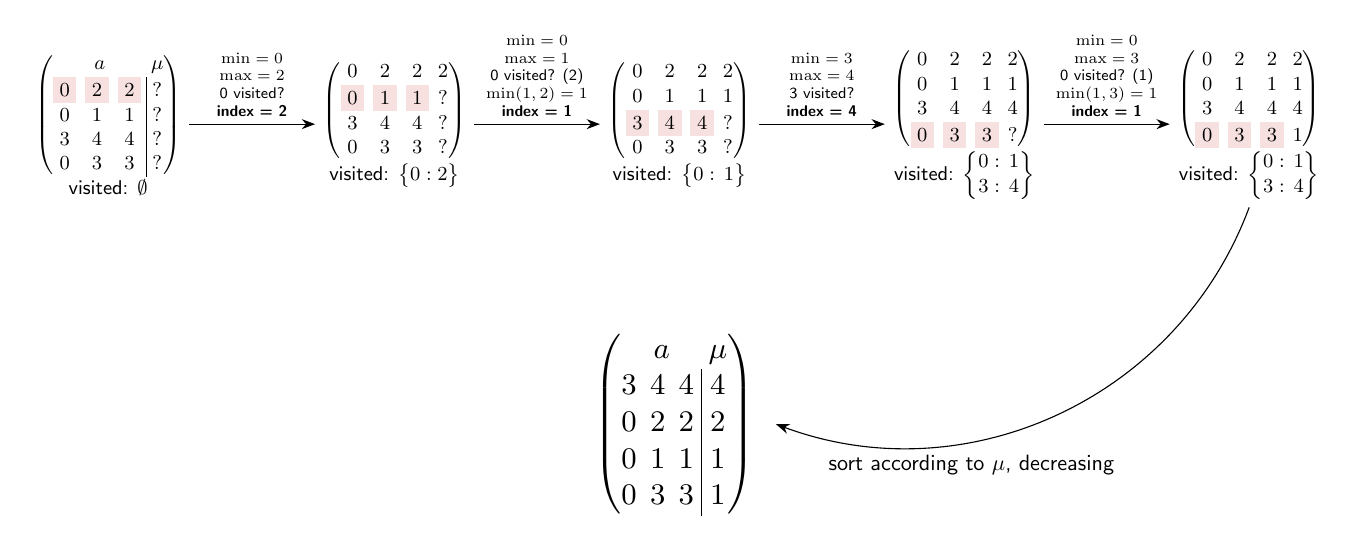
\begin{tikzpicture}[
        node distance=2cm,
        block/.style={
            minimum width=2cm,
            align=center,
            draw=none,
            font=\small
        },
        >=Stealth,
        scale=0.8, every node/.style={transform shape}
    ]

    % Define nodes for each step
    \node (step0) [block] {
        $\left(\begin{array}{@{}ccc|c@{}} 
            \multicolumn{3}{c}{\bm{a}} & \bm{\mu} \\
            \colorbox{Mahogany!10}{$0$} & \colorbox{Mahogany!10}{$2$} & \colorbox{Mahogany!10}{$2$} & ? \\ 
            0 & 1 & 1 & ? \\ 
            3 & 4 & 4 & ? \\ 
            0 & 3 & 3 & ? 
        \end{array}\right)$ \\
        visited: $\emptyset$
    };

    \node (step1) [block, right=2cm of step0] {
        $\begin{pmatrix} 
            0 & 2 & 2 & \Mahogany{2} \\ 
            \colorbox{Mahogany!10}{$0$} & \colorbox{Mahogany!10}{$1$} & \colorbox{Mahogany!10}{$1$} & ? \\
            3 & 4 & 4 & ? \\ 
            0 & 3 & 3 & ? 
        \end{pmatrix}$ \\
        visited: $\begin{Bmatrix}
            0: 2
        \end{Bmatrix}$
    };

    \node (step2) [block, right=2cm of step1] {
        $\begin{pmatrix} 
            0 & 2 & 2 & 2 \\
            0 & 1 & 1 & \Mahogany{1} \\
            \colorbox{Mahogany!10}{$3$} & \colorbox{Mahogany!10}{$4$} & \colorbox{Mahogany!10}{$4$}& ? \\ 
            0 & 3 & 3 & ? 
        \end{pmatrix}$ \\
        visited: $\begin{Bmatrix}
            0: & 1
        \end{Bmatrix}$
    };

    \node (step3) [block, right=2cm of step2] {
        $\begin{pmatrix} 
            0 & 2 & 2 & 2 \\
            0 & 1 & 1 & 1 \\
            3 & 4 & 4 & 4 \\
            \colorbox{Mahogany!10}{$0$} & \colorbox{Mahogany!10}{$3$} & \colorbox{Mahogany!10}{$3$} & ? 
        \end{pmatrix}$ \\
        visited: $\begin{Bmatrix}
            0: & 1 \\
            3: & 4 \\
        \end{Bmatrix}$
    };

    \node (step4) [block, right=2cm of step3] {
        $\begin{pmatrix} 
            0 & 2 & 2 & 2 \\
            0 & 1 & 1 & 1 \\
            3 & 4 & 4 & 4 \\
            \colorbox{Mahogany!10}{$0$} & \colorbox{Mahogany!10}{$3$} & \colorbox{Mahogany!10}{$3$} & \Mahogany{1} \\
        \end{pmatrix}$ \\
        visited: $\begin{Bmatrix}
            0: & 1 \\
            3: & 4 \\
        \end{Bmatrix}$
    };

    \node[scale=1.5, transform shape] (output) [block, below=2cm of step2] {
        $\left(\begin{array}{@{}ccc|c@{}} 
            \multicolumn{3}{c}{\bm{a}} & \bm{\mu} \\
            3 & 4 & 4 & 4 \\ 
            0 & 2 & 2 & 2 \\ 
            0 & 1 & 1 & 1 \\ 
            0 & 3 & 3 & 1 
        \end{array}\right)$
    };

    \draw [->] (step0.east) to node[midway, above, align=center, font=\scriptsize] {
        $\min = 0$ \\ 
        $\max = 2$ \\ 
        0 visited? \xmark \\
        \textbf{index = 2}
      }  (step1.west);
    \draw [->] (step1.east) to node[midway, above, align=center, font=\scriptsize] {
        $\min = 0$ \\ 
        $\max = 1$ \\ 
        0 visited? \cmark (2) \\
        $\min(1, 2) = 1$ \\
        \textbf{index = 1}
      } (step2.west);
    \draw [->] (step2.east) to node[midway, above, align=center, font=\scriptsize] {
        $\min = 3$ \\ 
        $\max = 4$ \\ 
        3 visited? \xmark \\
        \textbf{index = 4}
      } (step3.west);
    \draw [->] (step3.east) to node[midway, above, align=center, font=\scriptsize] {
        $\min = 0$ \\ 
        $\max = 3$ \\ 
        0 visited? \cmark (1) \\
        $\min(1, 3) = 1$ \\
        \textbf{index = 1}
      } (step4.west);
    \draw [->, bend left=45] (step4.south) to node[pos=0.66, yshift=-0.1cm, below, align=center] {sort according to $\bm{\mu}$, decreasing} (output.east);
    \end{tikzpicture}
    \caption{Illustration of Algorithm~\ref{alg:order_cherries}, using the output from Fig.~\ref{fig:parse-snake}.}
    \label{fig:ordercherries}
\end{figure}

The obtained ordered ancestry mirrors the cherry list in Algorithm~\ref{alg:to_pairs}. To infer the inverse operation and finally recover a phylo2vec vector \v, we observe that each cherry (the first two columns of the ancestry) comprises a newly added leaf (right) and its smallest descendant (left). To infer the branch from which the added leaf $\ell_{add}$ descends, we must count the number of leaves that have already been placed with labels smaller than $\ell_{add}$. To this end, we employ Fenwick trees~\cite{ryabko1992, fenwick1994}, which support dynamic prefix-sum queries to track the number of earlier placements. A sketch of the algorithm implemented by Scheidwasser \textit{et al.}~\cite{scheidwasser2025} is presented in Algorithm~\ref{alg:buildvector}, with an illustrated example in Fig. ~\ref{fig:build_vector}.

\begin{algorithm}[htbp]
\begin{algorithmic}[1]
\Require $\bm{a}$ \Comment{Ordered ancestry}

\Comment{$\bm{a}$ is of length $n-1$ with $n$ the number of leaves}
\State $\bm{f} = \begin{pmatrix}
    0 & 0 & ...
\end{pmatrix}$ \Comment{Fenwick tree data. Length: $n-1$}
\State $\bm{v} = \begin{pmatrix}
    0 & 0 & ...
\end{pmatrix}$ \Comment{Length: $n-1$}
\For{$j \gets 0$ \textbf{to} $n - 2$}
    \State $c_m \gets \min(\bm{a}_j), c_M \gets \max(\bm{a}_j)$
    \State $i \gets \bm{f}_\Sigma(c_M-1)$ \Comment{Fenwick prefix sum}
    \If{$i = 0$} 
        \State $\bm{v}_{c_M-1} = c_m$ 
    \Else
        \State $\bm{v}_{c_M-1} = c_M - 1 + \bm{f}_\Sigma(c_M-1)$ 
    \EndIf
    \State $\bm{f}$.update($c_M$, 1) \Comment{Fenwick update}
\EndFor
\State \Return $\bm{v}$
\end{algorithmic}
\caption{Build a phylo2vec vector from an ordered ancestry.}
\label{alg:buildvector}
\end{algorithm}

\begin{figure}[htbp]
    \centering
    \setlength{\arraycolsep}{2pt}
    \begin{tikzpicture}[
        node distance=2cm,
        block/.style={
            minimum width=2cm,
            align=center,
            draw=none,
            font=\small
        },
        >=Stealth,
        scale=0.75, every node/.style={transform shape}
    ]

    % Define nodes for each step
    \node (input) [block, below=1.6 cm of step2] {
        $
        \begin{aligned}
        \bm{a} &= 
        \begin{pmatrix}
            \colorbox{Mahogany!10}{$3$} & \colorbox{Mahogany!10}{$4$} & \colorbox{Mahogany!10}{$4$} \\ 
            0 & 2 & 2 \\ 
            0 & 1 & 1 \\ 
            0 & 3 & 3 
        \end{pmatrix} \\
        \bm{f} &= 
        \begin{pmatrix}
            0 & 0 & 0 & 0 & 0 \\
        \end{pmatrix} \\
        \bm{v} &= 
        \begin{pmatrix}
            0 & 0 & 0 & 0\\
        \end{pmatrix}
        \end{aligned}
        $
    };

    \node (step1) [block, right=1.6 cm of input] {
        $
        \begin{aligned}
        \bm{a} &= 
        \begin{pmatrix}
            3 & 4 & 4 \\ 
            \colorbox{Mahogany!10}{$0$} & \colorbox{Mahogany!10}{$2$} & \colorbox{Mahogany!10}{$2$} \\ 
            0 & 1 & 1 \\ 
            0 & 3 & 3 
        \end{pmatrix} \\
        \bm{f} &= 
        \begin{pmatrix}
            0 & 0 & 0 & 0 & 1 \\
        \end{pmatrix} \\
        \bm{v} &= 
        \begin{pmatrix}
            0 & 0 & 0 & \Mahogany{3} \\
        \end{pmatrix}
        \end{aligned}
        $
    };

    \node (step2) [block, right=1.6 cm of step1] {
        $\begin{aligned}
        \bm{a} &= 
        \begin{pmatrix}
            3 & 4 & 4 \\ 
            0 & 2 & 2 \\ 
            \colorbox{Mahogany!10}{$0$} & \colorbox{Mahogany!10}{$1$} & \colorbox{Mahogany!10}{$1$} \\ 
            0 & 3 & 3 
        \end{pmatrix} \\
        \bm{f} &= 
        \begin{pmatrix}
            0 & 0 & 1 & 0 & 2 \\
        \end{pmatrix} \\
        \bm{v} &= 
        \begin{pmatrix}
            0 & \Mahogany{0} & 0 & 3 \\
        \end{pmatrix}
        \end{aligned}
        $
    };

    \node (step3) [block, right=1.6 cm of step2] {
        $
        \begin{aligned}
        \bm{a} &= 
        \begin{pmatrix}
            3 & 4 & 4 \\ 
            0 & 2 & 2 \\ 
            0 & 1 & 1 \\ 
            \colorbox{Mahogany!10}{$0$} & \colorbox{Mahogany!10}{$3$} & \colorbox{Mahogany!10}{$3$}
        \end{pmatrix} \\
        \bm{f} &= 
        \begin{pmatrix}
            0 & 1 & 2 & 0 & 3 \\
        \end{pmatrix} \\
        \bm{v} &= 
        \begin{pmatrix}
            \Mahogany{0} & 0 & 0 & 3 \\
        \end{pmatrix}
        \end{aligned}
        $
    };

    \node (step4) [block, right=2.1 cm of step3] {
        $
        \begin{aligned}
        \bm{v} &= 
        \begin{pmatrix}
            0 & 0 & \Mahogany{4} & 3 \\
        \end{pmatrix}
        \end{aligned}
        $
    };

    \draw[->] (input.east) to node[midway, above, align=center, font=\scriptsize] {
    $
    \begin{aligned}
        \min              &= 3 \\
        \max              &= 4 \\
        \bm{f}_\Sigma(4-1) &= 0 \\
        \bm{v}_{4-1}      &= 3
    \end{aligned}
    $
    }  (step1.west);

    \draw[->] (step1.east) to node[midway, above, align=center, font=\scriptsize] {
        $\begin{aligned}
        \min              &= 0 \\
        \max              &= 2 \\
        \bm{f}_\Sigma(2-1) &= 0 \\
        \bm{v}_{2-1}      &= 0
      \end{aligned}$
    }  (step2.west);

    \draw[->] (step2.east) to node[midway, above, align=center, font=\scriptsize] {
        $
        \begin{aligned}
            \min            &= 0 \\
            \max            &= 1 \\
            \bm{f}_\Sigma(1-1) &= 0 \\
            \bm{v}_{1-1}    &= 0
        \end{aligned}
        $
      }  (step3.west);

    \draw[->] (step3.east) to node[midway, above, align=center, font=\scriptsize] {
        $
        \begin{aligned}
            \min &= 0 \\ 
            \max &= 3 \\ 
            \bm{f}_\Sigma(3-1) &= 2 \\ 
            \bm{v}_{3-1} = 3 - 1 + 2 &= 4
          \end{aligned}
        $   
      }  (step4.west);

    \end{tikzpicture}
    \caption{Building a vector from an ordered ancestry $\bm{a}$, using the output of Fig.~\ref{fig:ordercherries} as an example. $\bm{f}$ denotes the prefix sum data collected at each iteration in Algorithm~\ref{alg:buildvector}. The $-1$ in $\bm{f}$ and $\bm{v}$ are due to 0-indexing. For a given cherry $(c_m, c_M)$ at position $j$, $\bm{f}_\Sigma(c_M)$ is equivalent to the number of cherries $(c_1, c_2)$ at position $i < j$ such that $c_2 \leq c_M$. If $\bm{f}_\Sigma(c_M) = 0$, $(c_m, c_M)$ is an ``ordered" cherry. Thus, $c_M$ descends from $c_m$ and $\bm{v}_{c_M-1} = c_m$. Otherwise, $c_M$ descends from an internal branch. In this case, $\bm{v}_{c_M-1}$ is calculated as the number of leaves before $c_M$ is added (i.e., $c_M - 1$) + $\bm{f}_\Sigma(c_M)$: $\bm{v}_{c_M-1} = c_M - 1 + \bm{f}_\Sigma(c_M)$.}
    \label{fig:build_vector}
\end{figure}

\subsection{Complexity}

\begin{table}[htbp]
    \centering
    \small
    \caption{Complexity of phylo2vec conversion algorithms. $n$: number of leaves in the rooted binary tree. By default, the average complexity is displayed in the ``Time complexity" column. If the best-case or the worst-case complexity differ, they are respectively highlighted in green and red.}
    \begin{tabular}{lllc}
        \toprule
        Algorithm & Pipeline & Ref. & Time complexity ($\bigO$) \\
        \midrule
        \multicolumn{4}{c}{\v~$\rightarrow$ Newick} \\
        \midrule
         Form a post-order-like list of cherries & \v~$\rightarrow \bm{p}$ & Algorithm~\ref{alg:to_pairs}; Fig.~\ref{fig:to_pairs} & $n \log n$ (\colorbox{green!10}{$n$}) \\
         Build a Newick string from $\bm{p}$ & $\bm{p} \rightarrow$ Newick & Fig.~\ref{fig:build_newick} & $n \sqrt n$ $\big($\colorbox{green!10}{$n \log n$}, \colorbox{red!10}{$n^2$}$\big)$ \\
         \midrule
         \multicolumn{4}{c}{Newick $\rightarrow$ \v} \\
         \midrule
         Parse a Newick string & Newick $\rightarrow \bm{a}$ & Fig.~\ref{fig:parse-snake} & $n$ \\
         Order $\bm{a}$ & $\bm{a}\rightarrow \bm{a}$ & Algorithm~\ref{alg:order_cherries}; Fig.~\ref{fig:ordercherries} & $n$ $\big(\colorbox{red!10}{$n\log n$}\big)$ \\
         Build a vector & $\bm{a} \rightarrow$ \v & Algorithm~\ref{alg:buildvector}
         ; Fig.~\ref{fig:build_vector} & $n \log n$ \\
         \bottomrule
    \end{tabular}
    \label{tab:cpxity}
\end{table}

Table~\ref{tab:cpxity} summarises the complexity of the different algorithms to convert a phylo2vec vector \v to a Newick string and vice versa.

\subsubsection{Cherry list}

The naive implementation presented in Algorithm~\ref{alg:to_pairs} has a best-case complexity of $\bigO(n)$ for ordered vectors $\big($only \texttt{append} operations, which are $\bigO(1)\big)$, and a worst-case complexity of $\bigO(n^2)$ for completely unordered vectors $\big($only \texttt{insert} operations, which are $\bigO(n)\big)$. As $n$ grows, the ratio of leaf placements which satisfy $v_j < j$ tends to $1/2$, thus making the average complexity $\bigO(n^{1.5})$ or $\bigO(n\sqrt{n})$. An optimised implementation~\cite{scheidwasser2025} makes use of \gls{avl} trees~\cite{adelson1962}, a self-balancing binary search tree where insert operations are $\bigO(\log n)$ regardless of the insertion position. Thus, the best, average, and worst-case complexities of an \gls{avl}-based algorithm are $\bigO(n \log n)$. With that in mind, the current version of the \texttt{phylo2vec} package~\cite{scheidwasser2025} employs the naive algorithm for ordered vectors $\big(\bigO(n)\big)$, and the \gls{avl}-based algorithm for non-ordered vectors $\big(\bigO(n\log n)\big)$ as $\log n$ grows less quickly than $\sqrt n$.

\subsubsection{Newick building}

In Fig.~\ref{fig:build_newick}, the complexity of the cache building step is $\bigO(n \log n)$, as the number of decimal digits in an integer $N$ is $\lfloor\log_{10} N\rfloor+1$. The second stage involves $n-1$ iterations (one per pair), making the time complexity linear to the number of steps. However, the actual time complexity largely depends on string concatenation operations, which are affected by the tree topology. We can distinguish a few scenarios to provide a rough estimate of the best-, average-, and worst-case complexities. On the one hand, imbalanced trees such as caterpillar trees $\big($e.g., \v~$= \begin{pmatrix} 0 & 0 & 0 & ... & 0\end{pmatrix}\big)$ will involve consecutive string concatenations with an ever growing string at $\kappa_0$, thus producing a worst-case complexity of $\bigO(n^2)$. Conversely, more balanced trees $\big($e.g., \v~$= \begin{pmatrix} 0 & 1 & 0 & 1 & ... & 0 & 1\end{pmatrix}\big)$ result in a more even distribution of the concatenation operations: each character will be copied at most $\bigO(\log n)$ times as it propagates up the tree levels, yielding a best-case complexity of $\bigO(n \log n)$. A reasonable estimate for the average complexity is $\bigO(n \sqrt n)$, as the average height of binary trees is $\bigO(\sqrt n)$~\cite{flajolet1982}.

\subsubsection{Newick parsing}

Because each character is examined at most once, the complexity of the parsing function is bounded by the length of the Newick string, resulting in a time complexity of $\bigO(L)$, where $L$ is the number of characters in the Newick string. Given that Newick format representations grow linearly with the number of leaves $n$, the time complexity of the algorithm can also be written as $\bigO(n)$.

\subsubsection{Ancestry sorting}

Both algorithms for ancestry sorting run in linear $\big(\bigO(n)\big)$ time. If the input Newick contains explicit parent labels, we can utilise the ancestry's parent column as a sorting index to reorder the ancestry rows. This is possible because the parent column contains unique internal labels $n, ..., 2(n-1)$. Conversely, Algorithm~\ref{alg:order_cherries} exploits local orderings to derive a sorting index, which is also performed in linear time. However, it requires a stable sorting step, making the time complexity of the full algorithm $\bigO(n\log n)$.

\subsubsection{Vector building}

As mentioned in Section~\ref{methods:newick2v}, building a vector from a sorted ancestry requires the implementation of Fenwick trees to track cherry placements. Both the prefix sum and updates are logarithmic operations, making the algorithm linearithmic in time $\big(\bigO(n\log n)\big)$.

\subsection{Phylo2Mat: extending phylo2vec vectors with branch length annotations}

Whereas the topology of a tree depicts the evolutionary relationships between different entities, branch lengths are essential for quantifying the amount of evolution that has occurred along each lineage. To incorporate this information, we extend the vector formulation of phylo2vec into a matrix (we call the resulting format \emph{phylo2mat}) with two columns for branch length annotations. The order of the branch lengths is relevant when unrolling \v~as an ancestry (see Section~\ref{methods:newick2v}). Fig.~\ref{fig:phylo2mat} shows an example of how to annotate a tree from a phylo2mat matrix. 

All conversion algorithms described in Sections~\ref{methods:v2newick} and ~\ref{methods:newick2v} are broadly applicable to \emph{phylo2mat} matrices. During cherry ordering (Algorithm~\ref{alg:order_cherries}), an additional step is required to make the matrix formulation invariant to cherry permutations. \newline For instance, the isomorphic Newick strings \texttt{((1:0.1,2:0.2)3:0.3);} and \texttt{((2:0.2,1:0.1)3:0.3)} should yield the same matrix. To this end, we enforce an extra row ordering step, whereby each triplet is sorted as $(c_1', c_2', p)$ such that the smallest descendant of $c_1'$ is smaller than that of $c_2'$. This operation, in addition to branch length parsing in Newick strings, incurs some additional overhead without however changing algorithm complexity.

\begin{figure}[htbp]
\centering
\adjustbox{valign=t}{
   \begin{tabular}{p{6cm}c}
        \toprule
         \v~$= \begin{pmatrix}
             0 & 0 & 4 & 3
         \end{pmatrix}$ with branch lengths represented in two rows $\bm{\beta_1}$ and $\bm{\beta_2}$ & \adjustbox{valign=t}{
         \m~=~
         $\left(\begin{array}{c|cccc}
         \bm{v} & 0 & 0 & 4 & 3 \\
         \bm{\beta}_1 & a_1 & b_1 & c_1 & d_1 \\
         \bm{\beta}_2 & a_2 & b_2 & c_2 & d_2 \\
        \end{array}\right)$
        } \\
        \midrule
        Branch lengths are attributed to edges using the ancestry matrix \\ BL(3, 5) = $a_1$ \newline BL(4, 5) = $a_2$ \newline ... \newline BL(7, 8) = $d_1$ \newline BL(5, 8) = $d_2$ & \adjustbox{valign=t}{
        $\bm{a} = \begin{bmatrix}
        \rn{c11}{3} & \rn{c12}{4} & \rn{p1}{5} & \rn{a1}{a_1} & \rn{a2}{a_2} \\
        0 & 2 & 6 & b_1 & b_2 \\
        6 & 1 & 7 & c_1 & c_2 \\
        \rn{c31}{7} & \rn{c32}{5} & \rn{p3}{8} & \rn{c1}{d_1} & \rn{c2}{d_2} \\
        \end{bmatrix}$}
        \begin{tikzpicture}[overlay,remember picture]
            \path[every node/.style={font=\sffamily\small}]
                (c11) edge[bend right, red] node [left] {} (a1)
                (p1) edge[bend right, red] node [left] {} (a1)
                (c12) edge[bend left, blue] node [left] {} (a2)
                (p1) edge[bend left, blue] node [left] {} (a2)
                (c31) edge[bend left, red] node [left] {} (c1)
                (p3) edge[bend left, red] node [left] {} (c1)
                (c32) edge[bend right, blue] node [left] {} (c2)
                (p3) edge[bend right, blue] node [left] {} (c2);
        \end{tikzpicture} \\
        \midrule
        Annotated tree & \adjustbox{valign=t}{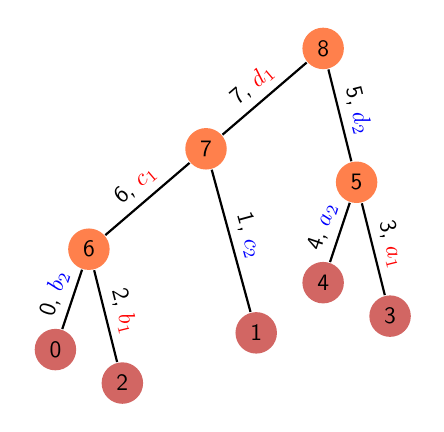
\begin{tikzpicture}[thick, scale=0.85, every node/.style={scale=0.85}]
            \node[circle, fill=Mahogany!50] (0) at (0, -0.5) {0};
            \node[circle, fill=Mahogany!50] (1) at (3, -0.25) {1};
            \node[circle, fill=Mahogany!50] (2) at (1, -1) {2};
            \node[circle, fill=Mahogany!50] (3) at (5, 0) {3};
            \node[circle, fill=Mahogany!50] (4) at (4, 0.5) {4};
            \node[circle, fill=Peach] (5) at (4.5, 2) {5};
            \node[circle, fill=Peach] (6) at (0.5, 1) {6};
            \node[circle, fill=Peach] (7) at (2.25, 2.5) {7};
            \node[circle, fill=Peach] (8) at (4, 4) {8};

            \draw (8) -- node[midway, sloped, above] {{5, \textcolor{blue}{$d_2$}}} (5);
            \draw (8) -- node[midway, sloped, above] {{7, \textcolor{red}{$d_1$}}} (7);
            \draw (7) -- node[midway, sloped, above] {{6, \textcolor{red}{$c_1$}}} (6);
            \draw (6) -- node[midway, above, sloped] {{2, \textcolor{red}{$b_1$}}} (2);
            \draw (7) -- node[midway, sloped, above] {{1, \textcolor{blue}{$c_2$}}} (1);
            \draw (6) -- node[midway, sloped, above] {{0, \textcolor{blue}{$b_2$}}} (0);
            \draw (5) -- node[midway, sloped, above] {{3, \textcolor{red}{$a_1$}}} (3);
            \draw (5) -- node[midway, sloped, above] {{4, \textcolor{blue}{$a_2$}}} (4);
        \end{tikzpicture}}\\
        \bottomrule
    \end{tabular}
}
\caption{Visual representation of an extended version of the phylo2vec vector with branch lengths, using \v~$= \begin{pmatrix}
    0 & 0 & 4 & 3
\end{pmatrix}$ as an example. Adapted from Scheidwasser \textit{et al.}~\cite{scheidwasser2025}.}
\label{fig:phylo2mat}
\end{figure}

\subsection{Implementation}

The original version of phylo2vec~\cite{penn2025} was implemented purely in Python, using \texttt{NumPy}~\cite{harris2020} for vector operations and \texttt{numba}~\cite{lam2015} to optimize NumPy-based functions using just-in-time compilation. The current implementation (v1.4.0)~\cite{scheidwasser2025} features several optimisations from an algorithmic (\gls{avl} tree-based conversion from \v~to Newick and Fenwick tree-based conversion from Newick to \v) and computational efficiency point of view, with core functions written in Rust~\cite{rust}. Rust was chosen as a core language because of its high performance, memory safety, and interoperability with other high-level programming languages. In particular, all core functions are available in dedicated Python and R packages via bindings implemented using \texttt{PyO3} (\url{https://pyo3.rs/v0.25.1/}) and \texttt{rextendr}~\cite{wilke2025}, respectively. In addition, we provide comprehensive documentation with notebook-based demos using \texttt{Read the Docs} (\url{https://about.readthedocs.com/}), and a robust pipeline for continuous integration (CI) and continuous delivery (CD) using GitHub Actions (\url{https://docs.github.com/en/actions/get-started/understand-github-actions}) to ensure reliable deployments while maintaining high code quality.

% \subsubsection{Maintenance and status of the software}
% Workshop, plans to delve deeper into inference-based operations.

\subsubsection{Other operations}

In addition to Newick conversion and branch length incorporation, we provide several other operations for manipulating trees using phylo2vec and phylo2mat objects. First, we provide several conversion functions of phylo2vec vectors (resp. phylo2mat matrices) to other objects used in phylogenetics, such as phylogenetic variance-covariance matrices, precision matrices (inverse of the phylogenetic variance-covariance matrix), and cophenetic distance matrices, using algorithms inspired by the \texttt{ape}~\cite{paradis2019} and \texttt{MCMCglmm}~\cite{hadfield2010} packages. Second, we added several operations on trees, such as leaf pruning and finding the \gls{mrca} of two nodes. Third, we provide skeletons for phylogenetic inference using phylo2vec and phylo2mat objects, in particular GradME~\cite{penn2023}, a gradient-based optimisation framework for distance-based phylogenetics using \gls{bme}~\cite{pauplin2000}, and a simple hill-climbing scheme akin to likelihood-based inference~\cite{penn2025} (see Section~\ref{methods:p2v_inference}). Finally, we provide a command-line interface (CLI) for rapid experimentation and compression of Newick trees into phylo2vec-derived objects.

\subsection{Properties}

We assess four properties of phylo2vec-derived objects: compression ratio (i.e., how much space is saved by compressing a Newick string into a phylo2vec vector), sampling speed, comparison speed (e.g., how fast is it to remove duplicate trees), and a simple tree distance metric calculated as a Hamming distance between vectors: $\bm{d}(\bm{v}, \bm{w}) = \sum_{j=0}^{n-2} \mathbb{I}_{\bm{v}_j\neq\bm{w}_j}$.

Benchmarks of the compression ratio and sampling speed were performed on the Python endpoint from $n$ = 10,000 to $n$ = 100,000 leaves. The compression ratio was assessed on Newick strings with and without branch lengths, and with taxon labels instead of integers. Sampling speed was assessed against \texttt{ape}~\cite{paradis2019} (\textcolor{red}{v5.x}) in R and \texttt{ete}~\cite{huerta2016} (\textcolor{red}{v4.x}) in Python. The comparison speed was benchmarked against \texttt{ape} on a task where the goal was to deduplicate a set of 100 trees where $n$ varied from 5 to 1,000 leaves. Finally, the phylo2vec-derived tree distance metric was benchmarked against other traditional distance measures, such as the number of \gls{spr} moves, as well as the \gls{rf}~\cite{robinson1981} and \gls{kf}~\cite{kuhner1994} distances. Distances were calculated between an initial vector \v with 200 leaves and 5,000 variations issued from a random walk starting from \v.

\subsection{Phylogenetic inference possibilities}
\label{methods:p2v_inference}
To evaluate the potential of phylo2vec vectors as base objects for phylogenetic inference, we devised a simple hill-climbing scheme
To evaluate the potential of phylo2vec as a basis for phylogenetic inference operations, we devised a simple hill-climbing scheme in which a single iteration consists of picking an index $j$ of $v$, swapping its value $v_j$ for a new value $v_j'$ randomly sampled according to the phylo2vec constraints (Eq. ~\ref{eq:p2v}). At the end of a single iteration, we performed branch length optimisation using RAxML-NG~\cite{kozlov2019} and calculated the likelihood of the new tree. These two operations were repeated until convergence (i.e. no improvement in the likelihood over three passes). To avoid getting stuck in local minima, we also include a ``shuffling" step, whereby the leaf label of each taxon is shuffled. This produces a new vector while maintaining the same tree topology, which enables the exploration of a new part of the vector space to escape local minima.

\subsubsection{Evaluation}
We evaluated the hill-climbing scheme described in Section~\ref{methods:p2v_inference} on four simple datasets as a proof of concept. These are composed of two hemagglutinin \glspl{msa} from influenza A viruses~\cite{sagulenko2018, fourment2019}, one \gls{msa} of Zika genomes~\cite{sanger1959}, and a datasets from parasitic worms (\textit{Acanthocephala}) containing 18S rRNA gene sequences~\cite{Garey1996-jc}.  

\clearpage
\section{Study 2: bcov3d}
The overarching goal of this study was to evaluate the informational utility of structure-based phylogenetics to complement our understanding of viral evolution. To this end, we gathered experimental spike glycoprotein structures from the \gls{pdb}~\cite{berman2000, rose2010} of various species of the \textit{Betacoronavirus} genus. We used Foldseek~\cite{vankempen2024} to translate the structures into discrete sequences and used MAST~\cite{wong2024} to analyse how recombination of binding domains shapes the structural evolution of spike proteins. 

\subsection{Data}
We based our protein structure dataset on a previously published collection of coronavirus structures called Cov3D~\cite{gowthaman2021}. We augment this dataset by performing sequence similarity searches in \gls{pdb}, using a cut-off of 50\% for 6 structures: 6VXX (SARS-CoV-2, wildtype)~\cite{walls2020}, 9CRH (SARS-CoV-2, Delta)~\cite{ke2024}, 8WHS (SARS-CoV-2, Omicron BA.2.86)~\cite{liu2024}, 6NB6 (SARS-CoV)~\cite{walls2019}, 8IFN (MERS-CoV)~\cite{tian2024}, 9BSW (HCoV-HKU1)~\cite{jin2025}, 7SB3 (HCoV-OC43)~\cite{bangaru2022}, 9K75 (BANAL-103)~\cite{qingqing2025}. This allowed us to include structures from various species within the betacoronavirus family~\cite{hu2021}. In total, we added $\approx$ 200 additional structures to the original Cov3D database, which had 1,932 structures as of June 2025. A summary of the protein structure metadata is presented in Table~\ref{table:bcov3d_counts}.

\begin{table}[htbp]
\centering
\caption{Distribution of \textit{Betacoronavirus} strains and variants in the study. For SARS-CoV-2, ``ambiguous" indicates that the variant was or could not be determined with certainty. In Cov3D~\cite{gowthaman2021}, they are typically named as ``Orig" or ``none", but the exact meaning of these labels is uncertain. Consequently, these structures were ignored in downstream analyses.}
\footnotesize
\begin{tabular}{lrlrlr}
\toprule
Strain (variant)               & Count & Strain (variant)               & Count & Strain (variant)               & Count \\
\midrule
SARS-CoV-2 (NS)       & 1108 & BatCoV RaTG13        & 3 & BtRs-BetaCoV/BtKY72            & 1 \\
SARS-CoV-2 (Omicron)  & 411  & BatCoV SHC014        & 3 & BtRs-BetaCoV/GX2013            & 1 \\
SARS-CoV-2 (Other)    & 184  & CN-HedgehogCoV HKU31 & 2 & BtRs-BetaCoV/YN2013            & 1 \\
SARS-CoV-2 (Delta)    & 100  & MCoV A59             & 2 & BtSY1                          & 1 \\
SARS-CoV              & 78   & BatCoV BM48-31       & 1 & Civet SARS CoV 007             & 1 \\
MERS-CoV              & 70   & BatCoV HKU5-20       & 1 & Civet SARS CoV SZ3             & 1 \\
HCoV-HKU1             & 50   & BatCoV RmyN02        & 1 & EU-HedgehogCoV                 & 1 \\
SARS-CoV-2 (Alpha)    & 44   & BatCoV BANAL-103     & 1 & MERS-like BtCoV/Ii/GD/2014-422 & 1 \\
SARS-CoV-2 (Wildtype) & 22   & BatCoV BANAL-52      & 1 & MERS-like PDF-2180             & 1 \\
HCoV-OC43             & 14   & BatCoV CX1           & 1 & PCoV GD                        & 1 \\
Bat SL-CoV-WIV1       & 6    & BatCov HKU25         & 1 & PCoV-GX                        & 1 \\
BatCoV HKU5           & 4    & BatCoV Vs-CoV 1      & 1 & PRD-0038                       & 1 \\
BatCoV BANAL-20-236   & 3    & BtCoV-422            & 1 & SA-BatCoV                      & 1 \\
BatCoV BANAL-20-52    & 3    & BtRf-BetaCoV/HeB2013 & 1 & SE-PangolinCoV MjHKU4r-Cov-1   & 1  \\
\bottomrule
\end{tabular}
\label{table:bcov3d_counts}
\end{table}


\subsection{Preprocessing}
A graphical summary of the preprocessing pipeline is shown in Fig.~\ref{fig:bcov3d_dag}.

\begin{figure*}[htbp]
    \centering
    \small
    \hspace{-0.5cm}%
    \begin{tikzpicture}[
        node distance=1.2cm,
        every node/.style={
            rectangle, 
            rounded corners,
            draw, 
            minimum width=2.5cm, 
            minimum height=0.6cm, 
            font=\footnotesize,
            align=center,
            fill=white
        },
        arrow/.style={-{Stealth[length=2mm]}},
        darrow/.style={
            -{Stealth[length=3mm]},
            dashed, line width=0.57mm,
        },
        dinterm/.style={
            dashed, line width=0.75mm,
        },
        scale=1.03
    ]
    
    % Background rectangles for each column
    \fill[RoyalBlue!20, rounded corners=5pt] (-3, 5.5) rectangle (3.25, -7.5);
    \fill[Peach!20, rounded corners=5pt] (3.25, 5.5) rectangle (7.75, -5);
    \fill[lime!20, rounded corners=5pt] (7.75, 5.5) rectangle (14, -5);
    \fill[Rhodamine!20, rounded corners=5pt] (3.25, -5) rectangle (14, -7.5);
    
    % Column headers
    \node[font=\bfseries\normalsize, fill=none, draw=none] (dataprep) at (-0.125, 5) {Dataset \\ preparation};
    \node[font=\bfseries\normalsize, fill=none, draw=none] (seqproc) at (5.5, 5) {Sequence \\ preprocessing};
    \node[font=\bfseries\normalsize, fill=none, draw=none] (phylo) at (10.875, 5) {Phylogenetic \\ analysis};
    \node[font=\bfseries\normalsize, fill=none, draw=none] (postproc) at (8.625, -5.5) {Post-processing};
    
    % Column 1 - Dataset preparation
    \node (raw) at (-0.125, 3.5) {Raw metadata};
    \node (aug) at (-0.125, 1.5) {Data augmentation};
    \node (download) at (-0.125, -0.5) {Download structures};
    \node (clean) at (-0.125, -4) {Cleaning \\ (remove short or \\ heteromeric structures)};
    \node (3di) at (-1.375, -6) {Extract \\ 3Di sequences};
    \node[minimum width=2cm] (aa) at (1.625, -6) {Extract \\ AA sequences};
    
    % Column 1 arrows
    \draw[arrow] (raw) -- (aug) node[midway, right, font=\small, fill=none, draw=none] {$n = 1,932$};
    \draw[arrow] (raw) -- (aug) node[midway, left, font=\scriptsize, fill=none, draw=none] {\textit{Cov3D}~\cite{gowthaman2021}};
    \draw[arrow] (aug) -- (download) node[midway, right, font=\small, fill=none, draw=none] {$n = 2,113$};
    \draw[arrow] (aug) -- (download) node[midway, left, font=\scriptsize, fill=none, draw=none] {\textit{PDB~\cite{rose2010} sequence} \\ similarity searches};
    \draw[arrow] (download) -- (clean) node[midway, left, font=\scriptsize, fill=none, draw=none] {\textit{biotite}~\cite{kunzmann2018}};
    \draw[arrow] (download) -- (clean) node[midway, right, fill=none, draw=none] {\includegraphics[width=2.1cm]{img/6VXX.png}};
    \draw[arrow] (clean) -- (3di);
    \draw[arrow] (clean) -- (aa) node[midway, right, font=\small, fill=none, draw=none] {$n = 676$};
    
    % Column 2 - Sequence preprocessing
    \node (align) at (5.5, 3.5) {Align};
    \node (trim) at (5.5, 2) {Remove gappy sites};
    \node (deduplicate) at (5.5, 0.5) {Deduplicate \\ (and drop gappy \\ sequences)};
    \node (subset) at (5.5, -1.25) {Subset @ x \\ Sample $x$ sequences \\ per virus/major variant};
    % \node (droplowgap) at (8, -1) {Drop gappy sequences};
    \node[minimum width=1.8cm] (subset1) at (4.5, -3.5) {Subset @ 1};
    \node[minimum width=1.8cm] (subset3) at (6.5, -3.5) {Subset @ 3};
    
    % Column 2 arrows
    \draw[arrow] (align) -- (trim) node[midway, left, font=\scriptsize, fill=none, draw=none] {\textit{MAFFT}~\cite{katoh2013}};
    \draw[arrow] (trim) -- (deduplicate) node[midway, left, font=\scriptsize, fill=none, draw=none] {\textit{trimal}~\cite{capella2009}};
    \draw[arrow] (deduplicate) -- (subset) node[midway, right, font=\small, fill=none, draw=none] {$n = 257$};
    \draw[arrow] (subset) -- (subset1) node[midway, left, xshift=0.4cm, font=\small, fill=none, draw=none] {$n = 36$};
    \draw[arrow] (subset) -- (subset3) node[midway, right, xshift=-0.4cm, font=\small, fill=none, draw=none] {$n = 62$};
    
    % Column 3 - Phylogenetic analysis
    \node[text width=2cm] (iqtreebase) at (12.5, 3.5) {Subset @ 3: \\determine substitution model};
    \node (cut) at (9.5, 3.5) {Subset @ 1: \\ cut sequences \\ into $m$ chunks \\ (150 residues)};
    \node (iqtreecut) at (11, 1.5) {Subset @ 1: \\ run IQ-TREE~\cite{minh2020} \\ on each chunked MSA};
    \node (maststart) at (11, -0.25) {Subset @ 1: \\ run MAST~\cite{wong2024} \\ using all $m$ trees};
    \node (mastiter) at (11, -2.25) {Subset @ 1: \\ repeat MAST with top \\ $m-1, \ldots, 2$ trees \\ w.r.t. likelihood};
    \node (bic) at (11, -4.25) {Model selection \\ (criterion: BIC)};
    
    % Column 3 arrows
    \draw[arrow] (iqtreebase) -- (iqtreecut) node[midway, right, xshift=-0.8cm, font=\tiny, fill=none, draw=none, color=black] {\textit{MFP}~\cite{kalyaanamoorthy2017}};
    \draw[arrow] (cut) -- (iqtreecut);
    \draw[arrow] (iqtreecut) -- (maststart);
    \draw[arrow] (iqtreebase) to [bend left=40] (maststart);
    \draw[arrow] (iqtreebase) to [bend left=45] (mastiter);
    \draw[arrow] (iqtreecut) to [bend right=65] (mastiter);
    \draw[arrow] (maststart) -- (mastiter);
    \draw[arrow] (mastiter) -- (bic);

    % Block 4 - postprocessing
    \node (domain) at (5.5, -6.5) {Protein domain \\ extraction};
    \node[fill=none, draw=none, font=\scriptsize] at (5.5, -7.1) {\textit{InterProScan}~\cite{jones2014}};
    \node (treefeat) at (11, -6.5) {Phylogenetic tree \\ feature extraction \\ (e.g., clock-likeness~\cite{zuckerkandl1962})};
    
    % Curved arrows between columns
    \draw[dinterm, blue!70] (aa.east) -- (3.25, -6);
    \draw[dinterm, blue!70] (3.25, -6) -- (3.25, 5);
    \draw[dinterm, blue!70] (3di.south) -- (-1.375, -7) node[midway, left, xshift=0.4cm, font=\scriptsize, fill=none, draw=none, color=black] {\textit{Foldseek}~\cite{vankempen2024}};
    \draw[dinterm, blue!70] (-1.375, -7) -- (3.25, -7);
    \draw[dinterm, blue!70] (3.25, -7) -- (3.25, -6);
    \draw[darrow, blue!70] (3.25, 5) -- (seqproc.west);
    \draw[dinterm, red!70] (subset3.east) -- (7.75, -3.5);
    \draw[dinterm, red!70] (subset1.south) -- (4.5, -4);
    \draw[dinterm, red!70] (4.5, -4) -- (7.75, -4);
    \draw[dinterm, red!70] (7.75, -4) -- (7.75, -1.5);
    \draw[dinterm, red!70] (7.75, -1.5) -- (7.75, 5);
    \draw[darrow, red!70] (7.75, 5) -- (phylo.west);
    \draw[darrow, red!70] (subset1.south) to [bend right=40] (domain.north);
    \draw[darrow, OliveGreen!80] (bic.south) to [bend left=40] (treefeat.north);
    
    \end{tikzpicture}
    \caption{Data processing and analysis workflow for the analysis of experimental spike glycoprotein structures from betacoronaviruses. The molecular structure image of PDB ID 6VXX~\cite{walls2019}, obtained from the RCSB PDB (\url{https://rcsb.org}) using Mol*~\cite{sehnal2021}, depicts a spike protein of a wild type SARS-CoV-2 bound with 2-acetamido-2-deoxy-beta-D-glucopyranose (NAG). MFP: ModelFinder Plus~\cite{kalyaanamoorthy2017}. BIC: Bayesian Information Criterion.}
    \label{fig:bcov3d_dag}
\end{figure*}

All structures were downloaded in mmCIF format using \texttt{biotite}~\cite{kunzmann2018}. Subsequently, we used Foldseek (v.10.941cd33)~\cite{vankempen2024} to translate each chain into a 3Di sequence for each protein structure in our database, after which we discarded all non-spike chains (e.g., antibodies or receptors). As the spike protein of coronaviruses consists of a homotrimer (i.e., three identical polypeptidic chains)~\cite{li2016} of approximately $1000-1200$ residues, we discarded spike structures that were either heteromeric or too short ($< 850$ residues). Although the length of a 3Di sequence will, on average, be slightly shorter than its \gls{aa} counterpart due to conformational disorders in the protein crystal~\cite{djinovic2015}, exceedingly short residues are likely to pose alignment issues for downstream phylogenetic analysis.

Second, we aligned the filtered sequences using \texttt{MAFFT}~\cite{katoh2013} with the \texttt{auto} and \texttt{leavegappyout} arguments, using the scoring matrix computed by Van Kempen \textit{et al.}~\cite{vankempen2024}. Gappy sites were trimmed from the aligned sequences using \texttt{trimal} (v1.5.rev0)~\cite{capella2009} with a gap threshold of 50\% (i.e., sites with gaps in 50\% or more of the sequences are removed). Finally, duplicate sequences were removed, yielding a set of 615 sequences.

Third, we processed the amino acid sequences from the deduplicated 3Di set. Similar to the 3Di pipeline, we used \texttt{MAFFT} and \texttt{trimal} for alignment and site trimming, respectively. The same parameters were used, except for the scoring matrix, where BLOSUM62~\cite{henikoff1992} was used. Additionally, we removed sequences where more than 50\% of sites were gaps, and ran a similar sequence deduplication process, yielding a set of 263 sequences.

Finally, we intersected the obtained 3Di and \gls{aa} sequence sets and retained one representative sequence per virus, except for SARS-CoV-2, for which we selected one sequence per major variant (Alpha, Delta, Omicron, wild type) and one sequence representing other variants (e.g., Beta, Kappa, Eta). For each virus and/or major variant, the representative sequence was the least gappy sequence of its group. The obtained subset comprised 36 sequences spanning three subgenera of betacoronaviruses (\textit{Sarbecovirus, Merbecovirus, Embecovirus}) which bind to various target receptors: angiotensin-converting enzyme 2 (ACE2), dipeptidyl peptidase-4 inhibitors (DPP4), and N-acetyl-9-O-acetylneuraminic acid receptors.

\subsection{Modelling}

We first assessed the phylogenetic signal in the \gls{aa} and 3Di datasets via an initial phylogenetic inference analysis using IQ-TREE (v2.4.0)~\cite{minh2020}. We used ModelFinderPlus (MFP)~\cite{kalyaanamoorthy2017} to determine the best substitution model $M_{best}$ for each dataset according to the \gls{bic}.

Subsequently, we performed an iterative mixture modelling analysis using MAST~\cite{wong2024} (available within the IQ-TREE suite) to determine the most suitable number of phylogenetic \emph{classes} that cluster the sequence sites in each dataset. To that end, for each MSA, we cut the sequences into $n$ regions, where $n$ varies from $2$ to $10$. Thereafter, we run IQ-TREE on each regional \gls{msa} using the substitution model $M_{best}$ to infer a phylogenetic tree for every region. We then run MAST using the $n$ obtained trees and the same substitution model before sorting the trees by weight. From this initial MAST run, we perform iterative runs using the same parameters, but only keeping the first $n - 1, n - 2, ..., 2$ trees. We compared all the MAST models using the \gls{bic} and the \gls{aicc} and displayed the preferable tree mixtures and site probabilities of the best models according to each criterion. The optimal number of classes according to each criterion is denoted as $c_{\gls{bic}}$ and $c_{\gls{aicc}}$, respectively.

\subsection{Phylogenetic tree analysis}
Using the best number of classes according to the \gls{bic}, we derived three tree statistics for the obtained tree mixture: tree length (the sum of all branch lengths), \emph{stemminess} (the ratio of internal branch lengths over total tree length)~\cite{fiala1985, rohlf1990}, and \emph{clock-likeness} (i.e., how stationary the rate of evolution is across lineages; measured as the variance of root-to-tip distances)~\cite{zuckerkandl1962, zuckerkandl1965}.

\subsection{Site-wise analysis}
\label{bcov3d:sitewise}
Using the best number of classes according to the \gls{bic} $c_{BIC}$, we obtain a probability distribution for each site to belong to the $c_{BIC}$ possible classes. Assuming that neighbouring sites should be fairly continuous, we smoothen the probabilities using a moving average filter with a window size of $w = 20$. This window size was deemed suitable for capturing domain-level trends as approximately equal to the length of the smallest domain in the spike protein (fusion peptide domain (FP))~\cite{huang2020}.

\subsection{Sequence feature extraction}

For each AA sequence in our subset, we inferred the coordinates of different biological domains within the set of \gls{aa} sequences using InterProScan~\cite{jones2014} (v5.75). Using information on missing amino acids in the protein structure from the \gls{pdb} files, we mapped the domain coordinates in the AA set to the coordinates in the 3Di sequence set using a custom script.

Finally, we derived the running average (with a window size of 20; see Section~\ref{bcov3d:sitewise}) of alignment entropy as well as site-wise averages on biophysical statistics, including hydrophobicity~\cite{kyte1982}, hydrophilicity~\cite{hopp1981}, and flexibility~\cite{vihinen1994} for the amino acid alignment. Hydrophilicity is expected to emphasise surface accessibility, which is essential for analysing the \gls{rbd}. Conversely, Kyte-Doolittle (KD) plots highlight the transmembrane domain of spike proteins. Finally, protein flexibility measures the degree to which different parts of a protein molecule can move or change their conformation.

\clearpage

\section{Study 3: chickens}
The last study of this thesis aimed to detect infection in poultry using a deep learning-based framework to analyse animal behaviour from video data. To that end, we designed a pilot study to assess welfare impairment from \textit{E. coli} infection in broiler chickens~\cite{scheidwasser2024}. Two groups of 20 broiler chickens, one control group and one group infected with \textit{E. coli} were monitored during the infection phase through video recordings. Using a deep neural network fine-tuned to track broilers, we extracted several kinematic features pertaining to behaviour: distance travelled, change in body area, and time spent near the food source. Using validation data from optical flow and physiological biomarkers of inflammation, we provide a proof-of-concept that deep learning-based, markerless tracking can be used for early detection of infection in poultry cohorts. We posit this approach constitutes a non-invasive, scalable approach to enhance flock health monitoring and biosecurity.

\subsection{Pilot \textit{E. coli} study}
\subsubsection{Experimental design}

A cohort of 40 day-old broiler chickens (Ross 308 breed; \textit{Gallus gallus domesticus}) was acquired and divided at random into two isolated groups: an \textit{E. coli}-infected group and a negative \textit{control} group. Both groups were reared for 38 days (Fig.~\ref{fig:setup}a) in 3.6 m $\times$ 2.4 m coops (Fig.~\ref{fig:setup}c). Each coop was equipped with a dust bath, two gravity-fed poultry drinkers providing water ad libitum, and a trough feeder replenished twice daily in accordance with standard recommendations~\cite{ross308, scheidwasser2024} 
(Fig.~\ref{fig:setup}c). On day 36, the infected group received an intratracheal inoculation with \textit{E. coli} strain ST117 E44, a pathogenic strain associated with colibacillosis in broilers~\cite{olsen2011, ronco2017, kromann2021}. In parallel, to control for handling-induced stress, chickens in the control group received an intratracheal sham inoculation with \gls{pbs}. Following inoculation, both groups were further observed for a 72-hour monitoring period. Initial visual checks of animal welfare were performed every 30 minutes for the first six hours, then at maximum eight-hour intervals. Predefined humane endpoints were established. If an individual presented with clinical signs such as ruffled feathers, depression, anorexia, lethargy, or dyspnea, it was first  treated with buprenorphine (0.1 mg/kg). Animals showing no improvement or deterioration post-treatment were euthanized according to predefined humane endpoints. On day 38, the animals were euthanised for biological data sampling by cervical dislocation immediately after being rendered unconscious by blunt head trauma.

\begin{figure}[htbp]
    \centering
    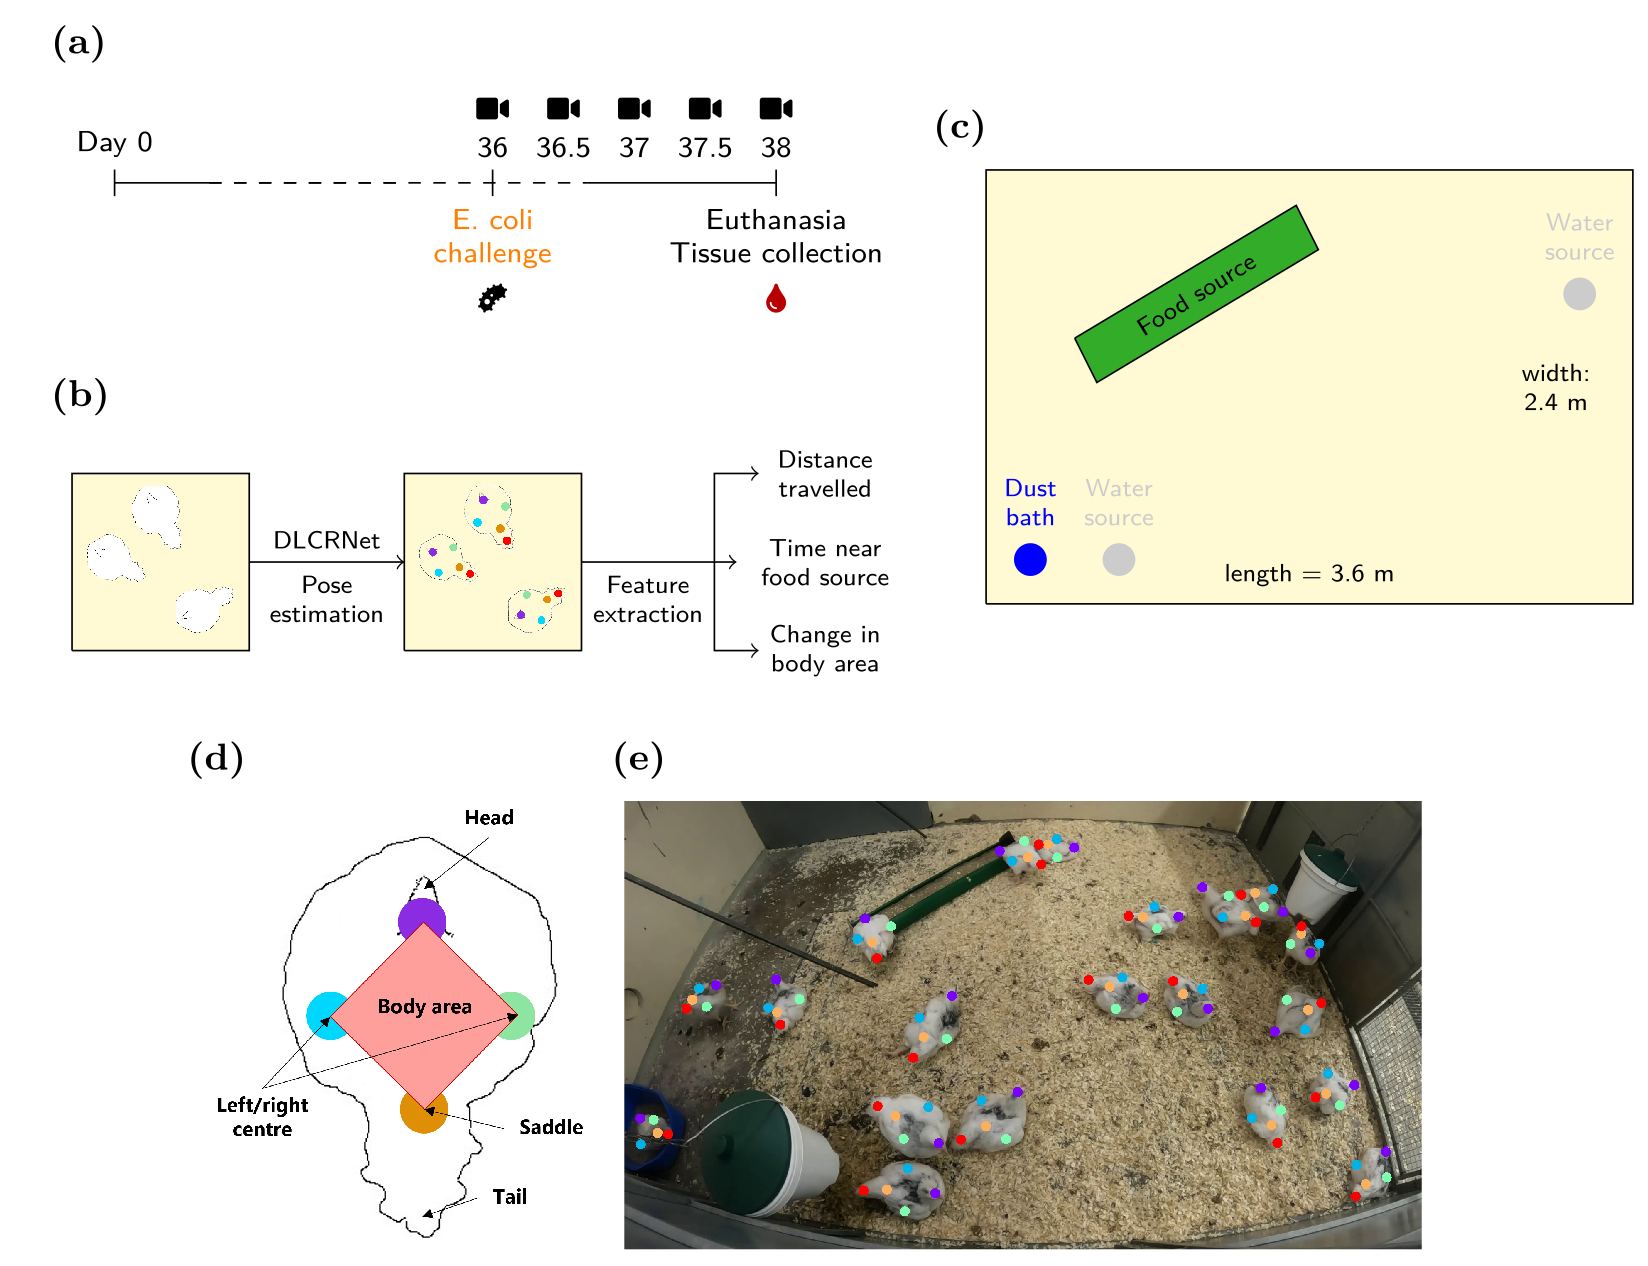
\includegraphics[width=0.9\linewidth]{img/chicken_rsos_fig1.png}
    \caption{Experimental setup. \textsb{(a)} Timeline of the experiment. \textsb{(b)} Pipeline for behavioural feature extraction using DLCRNet, the standard model of the multi-animal version of DeepLabCut (maDLC)~\cite{lauer2022}. \textsb{(c)} Diagram of the chicken coops. \textsb{(d)} Schematised top view of a broiler chicken with standardised body parts used for tracking and polygon used to approximate body area. \textsb{(e)} Example predictions from maDLC, based on one frame. Reproduced from Scheidwasser \textit{et al.}~\cite{scheidwasser2024}, used a Creative Commons Attribution License.}
    \label{fig:setup}
\end{figure}

\subsubsection{\textit{E. coli} and tissue sampling}

As the respiratory tract is a typical entry site for avian pathogenic \textit{E. coli}~\cite{dho1999} whereby an array of pulmonary symptoms are commonly observable~\cite{dho1999, nolan2013, kromann2021, liu2025}, bacteriological sampling was performed on both groups based on pulmonary sampling. For each animal, each lung was blended with a saline solution (1/1 (weight/vol) solution of 0.9\% \gls{pbs}) and subsequently plated into ten-fold serial dilutions to determine \glspl{cfu} via overnight incubation~\cite{scheidwasser2024}. To account for lung variability, \gls{cfu} counts were normalised by lung weight (unit: \textcolor{red}{unit}).

\subsubsection{Video monitoring}
\label{sec:chickenvideos}

Following the inoculation phase, 30-min videos were recorded every half-day (morning \& afternoon), totalling five videos over 2.5 days (Fig.~\ref{fig:setup}a). Video data was acquired using GoPro HERO10 Black cameras (\url{https://gopro.com}) placed on a wall 130 cm above each coop floor. To minimise behaviours induced by experimenter intervention, the first two minutes were removed from each video as the experimenter prepared the cameras. The frame resolution of each video was of 1080 $\times$ 1920 pixels and the frame rate 30 Hz. Thus, the video dataset totals approximately $2~\text{groups} \times 5~\text{videos} \times 30~\text{minutes} \times 60~\text{s/min} \times 30~\text{frames/s} = 540,000$ frames.

\subsubsection{Optical flow}

Optical flow was estimated was each video using SEA-RAFT~\cite{wang2025}, a state-of-the-art deep learning-based model trained to predict the \emph{flow map} (i.e., the $(x,y)$ motion of each pixel) between consecutive frames. To fit model requirements and speed up inference, video frames from Section~\ref{sec:chickenvideos} were downsampled by 50\% (540 $\times$ 960 pixels). In accordance with previous research~\cite{dawkins2009, dawkins2012, colles2016} we derived the first four statistical moments (mean, variance, skewness, and kurtosis) of each flow map and extracted the frame-wise average moment for each video.

\subsubsection{Deep learning-based tracking}

Animal tracking was performed using the DeepLabCut~\cite{mathis2018} toolkit. Following toolkit recommendations, a dataset of 100 frames was constructed by extracting 20 representative frames over five video segments using the unsupervised $k$-means algorithm. Each extracted frame was labelled by annotating the $(x,y)$ positions of five body parts (head, centre left, centre right, saddle, and tail; Fig.~\ref{fig:setup}d) for each broiler. Using this labelled dataset, we fine-tuned a pre-trained model for multi-animal pose estimation and tracking called \emph{DLCRNet\_ms5}~\citep{lauer2022} via end-to-end training with recommended hyperparameters from Lauer \textit{et al.}~\cite{lauer2022}. To evaluate model performance, we computed the root mean squared errors (RMSEs) of predicted body part positions against a held out test set of five frames. For input frames with a 1080 $\times$ 1920 pixels, the training and testing RMSEs were 3.03 pixels and 8.68 pixels, respectively. This performance was deemed satisfactory, we analysed all non-labelled frames to infer the animals' poses and body part positions. In a nutshell, the final tracking dataset consists of a five-dimensional tensor of $N \times F \times C \times B \times D$, where $N, F, C, B, D$ respectively denote the number of videos (10), the number of frames ($\approx 30 \times 60 \times 30 = 54,000$ per video), and the number of broiler chickens ($\approx 20$), the number of body parts (5), and $D = 3$ corresponds to the predicted $(x,y)$ position as well as the likelihood $L \in (0,1)$ of that prediction~\cite{scheidwasser2024}.

\subsubsection{Behavioural feature extraction}

Following recommendations from the DeepLabCut toolkit, we voided all predictions with a likelihood lower than 0.9. Data gaps smaller or equal than 15 frames (0.5 s) were recovered by applied forward linear interpolation, with the assumption that the movement in such a small interval would be small. All predicted positions were smoothened using Savitkzy-Golay filtering~\cite{savitzky1964} with a polynomial order of 7 and a window length of 15 frames to filter out outlier predictions and capture general locomotor trends for each body part~\cite{scheidwasser2024}. 

From this cleaned tracking dataset, we extracted three behavioural features for each chicken in each video: First, the \emph{travelled distance} of an animal (Eq.~\ref{eq:travel}) was estimated as the sum of displacements of its centre of mass (Eq.~\ref{eq:com} over consecutive frames. Second, the \emph{rate of change of body area} was measured as a proxy for measuring non-locomotor movement. The body area of an animal was approximated from a quadrilateral made of the head, the left centre, the right centre, and the saddle (Fig.~\ref{fig:setup}d). Third, the \emph{time spent near the food source} was extracted as a means to estimate feeding behaviour. It was estimated by calculating the percent of frames in each video for which the head of a given animal was in the vicinity of the food source~\cite{scheidwasser2024}. As the camera was placed at a high angle view instead of a bird's eye view, we normalized the two abovementioned features for each animal and frame by its body length, determined as the distance between the head and the saddle. 

\begin{align}
    L_{.,v,c} &= \sum_{i=1}^{N} \frac{\mathbf{d}(\centerofmass_{i,v,c} - \centerofmass_{i-1,v,c})}{\mathbf{d}(\text{head}_{i,v,c}, \text{saddle}_{i,v,c})} \\
    \label{eq:travel}
    \dot{A}_{.,v,c} &= \sum_{i=1}^{N} \frac{|\dot{A}_{i,v,c}|}{\mathbf{d}(\text{head}_{i,v,c}, \text{saddle}_{i,v,c})} \\
    \centerofmass_{i,v,c} &= \Big(\frac{1}{4}(x_{\text{i,v,c,head}} + x_{\text{i,v,c,centreleft}} + x_{\text{i,v,c,centreright}} + x_{\text{i,v,c,saddle}}),\notag\\ 
    &~~\frac{1}{4}(y_{\text{i,v,c,head}} + y_{\text{i,v,c,centreleft}} + y_{\text{i,v,c,centreright}} + y_{\text{i,v,c,saddle}})\Big)
    \label{eq:com}
\end{align}

\subsubsection{Statistical analysis}

\subsubsection{Implementation}

% \subsubsection{Pilot \textit{E. coli} study}
% We had to delete video data where we could see the technicians due to ethical concerns.

% % \subsection{Data sources}
% % \subsection{Study 1: phylogenetic trees}
% % Binary phylogenetic trees
% % \subsection{Study 2: protein structures}
% % Gene sequences
% % \subsection{Study 3: broiler chickens}
% % ross chickens
% % two weeks
% % \subsubsection{Pilot study}
% % Pilot study: 3 groups = control, e. coli, e. coli + vax
% % \subsubsection{Multipath study}
% % Multipath

% \subsection{\textit{C. jejuni} studies}
% Campy x2


% \subsection{Data processing}

\chapter{Results}
\section{Summarized results from Study 1}
The initial goal of this study was to derive new analysis frameworks for phylogenetics by representing phylogenetics as something more malleable, for example, a set of features for machine learning. This led to the development of \gls{p2v} (or Phylo2Vec)~\cite{penn2025, scheidwasser2025}, a framework for representing phylogenetic tree topologies as integer vectors. Inspired by Yule processes~\cite{steel2001} and tree counting strategies~\cite{knuth1973, rotem1978, proskurowski1980, rohlf1983}, the core idea of phylo2vec is to describe \emph{how} leaves are iteratively added to an existing tree topology. The construction of phylo2vec builds upon the work of Rohlf~\cite{rohlf1983} and Dinh~\cite{dinh2010}, but differs in its edge labelling strategy and, in the case of Rohlf~\cite{rohlf1983}, in preserving the tree-construction process within the vector representation. Beyond this conceptual shift, our contributions were fourfold: (i) rigorous proofs that the vector representation is bijective with the space of binary rooted trees~\cite{penn2025}, (ii) an extended matrix format to incorporate branch length information, (iii) empirical evidence of its usability for phylogenetic inference, and (iv) robust and open-source software for manipulating phylogenetic trees using this representation~\cite{scheidwasser2025}. % In addition, the simplicity of such a vector format makes it a convenient starting object for phylogenetic tree manipulation, which is showcased in the \texttt{phylo2vec} software package~\cite{scheidwasser2025}. The package also highlights potential avenues for phylo2vec-based phylogenetic inference, including non-traditional optimisation approaches such as (gradient-based \gls{bme} (GradME)~\cite{penn2023}.

% phylo2vec was originally designed with fast sampling, rapid comparison, and efficient compression of phylogenetic trees

The simple constraint of the phylo2vec formulation notably allows for rapid tree sampling, efficient compression, and straightforward comparison of tree topologies. As shown in Fig.~\ref{fig:p2v_sample}, it is notably faster than the widely used tree manipulation libraries \texttt{ete3}~\cite{huerta2016} and  \texttt{ape}~\cite{paradis2019} (Fig.~\ref{fig:p2v_sample}). The distribution of trees generated from phylo2vec sampling is also naturally uniform~\cite{scheidwasser2024}, similar to the proportional-to-distinguishable-arrangements model~\cite{holman2005}.

\begin{figure}[htbp]
    \centering
    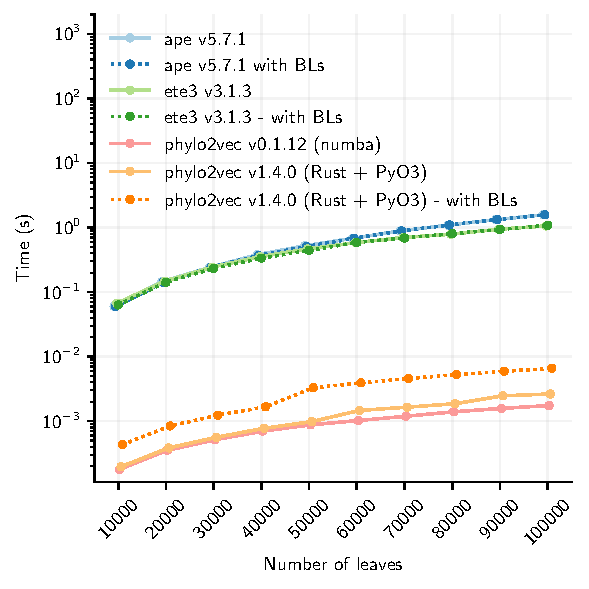
\includegraphics[width=0.5\linewidth]{img/sample_benchmark.pdf}
    \caption{Sampling speed of phylo2vec vectors and matrices. Plain lines denote functions for sampling a single random tree topology. Dotted lines denote functions for sampling a single random tree with random branch lengths (BLs).}
    \label{fig:p2v_sample}
\end{figure}

phylo2vec also allows for fast comparison of binary trees, as illustrated by the deduplication task in Penn \textit{et al.}~\cite{penn2025}. Beyond equality, two tree topologies can be compared using phylo2vec via a simple Hamming distance between their respective vectors, as described in Section~\ref{methods:p2v_properties}. Through random walks in both phylo2vec and tree spaces, we observed that moves in the phylo2vec space \emph{generally} equated with \gls{spr} rearrangements. Linear correlation with the Hamming distance was highest with the \gls{spr} distance (Pearson's $r$: 0.93), and lowest for distance metrics related to \gls{nni} (Fig.~\ref{fig:p2v_dist}). Yet, performing a single \gls{spr} on a tree may still result in a significantly different vector (Fig.~\ref{fig:p2v_metrics_from_moves}), and vice versa for a single vector move (Hamming distance of one) (Fig.~\ref{fig:p2v_metrics_from_v_single}).

\begin{figure}[htbp]
    \centering
    \subfloat[]{%
        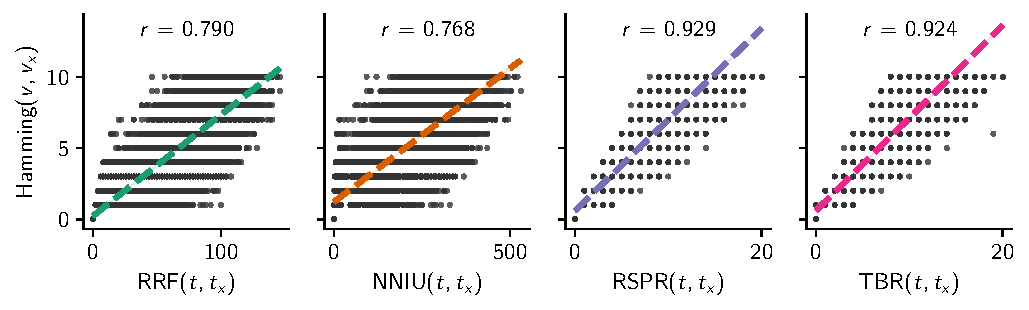
\includegraphics[height=6cm]{img/compare_metrics_from_v.pdf}%
        \label{fig:p2v_metrics_from_v}%
    }
    \subfloat[]{%
        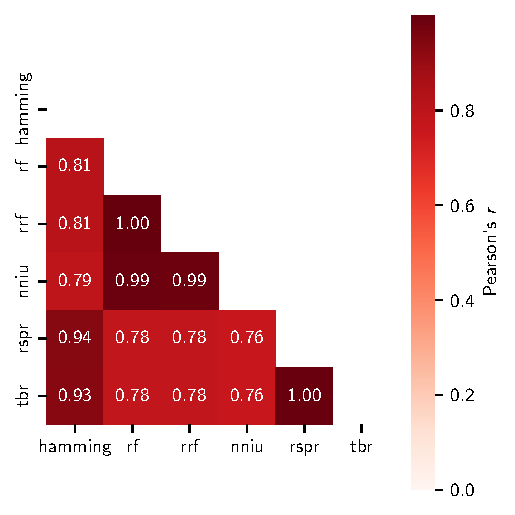
\includegraphics[height=6cm]{img/compare_metrics_from_v_corr.pdf}%
        \label{fig:p2v_metrics_corr}%
    } \\
    \subfloat[\label{fig:p2v_metrics_from_v_single}]{%
        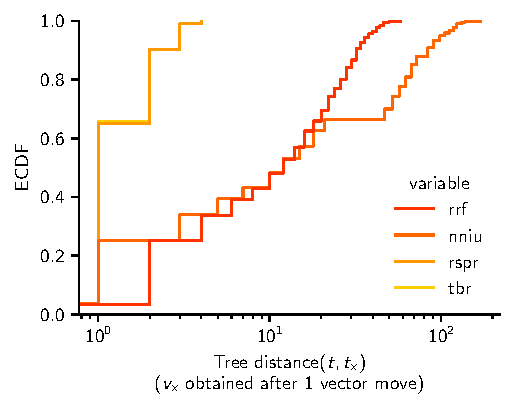
\includegraphics[height=5cm]{img/compare_metrics_from_v_single.pdf}%
        %
    }
    \subfloat[\label{fig:p2v_metrics_from_moves}]{%
        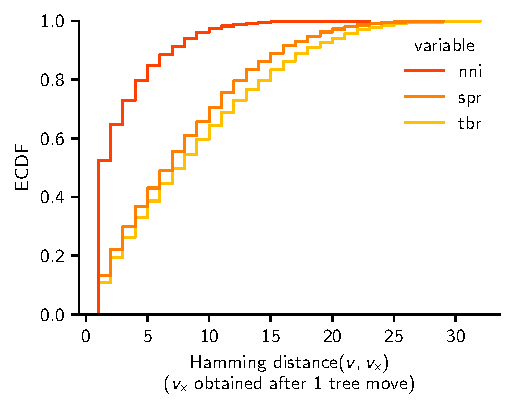
\includegraphics[height=5cm]{img/compare_metrics_from_moves.pdf}%
        %
    }
    \caption{Comparison of phylo2vec topology moves against standard tree rearrangement operations: \gls{nni}, \gls{spr}, \gls{tbr}.}
    \label{fig:p2v_dist}
\end{figure}

Due to its flat vector nature, an immediate property of phylo2vec is its compact format (Fig.~\ref{fig:p2v_compression}). For tree topologies, a phylo2vec vector occupies less memory than the Newick format for trees with 100 leaves or more, and the compression ratio reaches 6x using 16-bit integers (up to $\approx$ 32,000 leaves) and 3x using 32-bit integers (Fig.~\ref{fig:p2v_vs_nwk_int}). For trees with branch lengths, phylo2vec is preferable for large trees (10,000 leaves or more), where the compression ratio reaches 10x for 100,000 leaves (Fig.~\ref{fig:p2v_vs_nwk_float}).

Saving thousands of trees, an operation typically performed in Bayesian phylogenetics involving \gls{mcmc} sampling, can also be optimised using phylo2vec. Although standard file compression (e.g., using \texttt{gzip}) already enables some significant savings, saving 10,000 trees in phylo2vec format can be approximately 5 to 50 times more efficient in terms of file size than a plain-text counterpart (Fig.~\ref{fig:p2v_vs_nwk_int_files},~\ref{fig:p2v_vs_nwk_float_files}).

\begin{figure}[htbp]
    \centering
    % First row
    \subfloat[]{%
        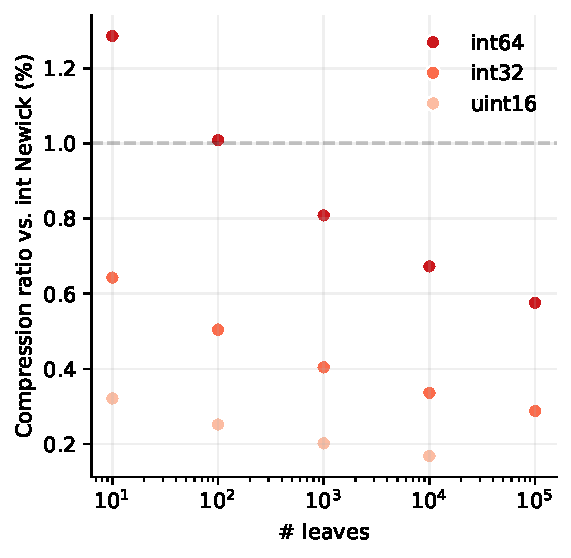
\includegraphics[width=0.4\textwidth]{img/p2v_vs_nwk_int.pdf}%
        \label{fig:p2v_vs_nwk_int}%
    }
    \hspace{0.25cm}
    \subfloat[]{%
        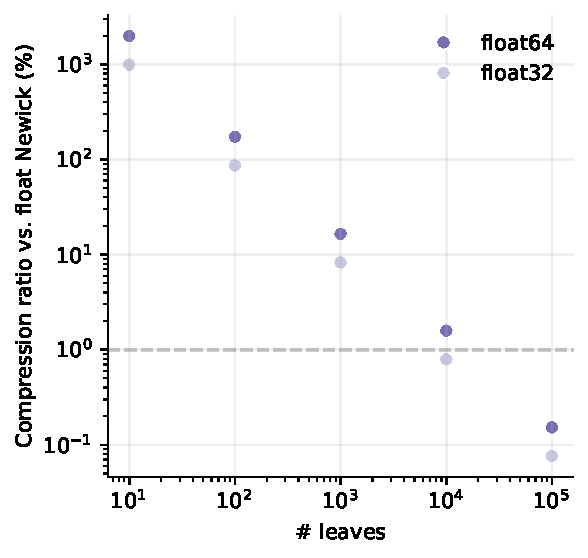
\includegraphics[width=0.4\textwidth]{img/p2v_vs_nwk_float.pdf}%
        \label{fig:p2v_vs_nwk_float}%
    }
    \vspace{0.25cm}
    % Second row
    \subfloat[]{%
        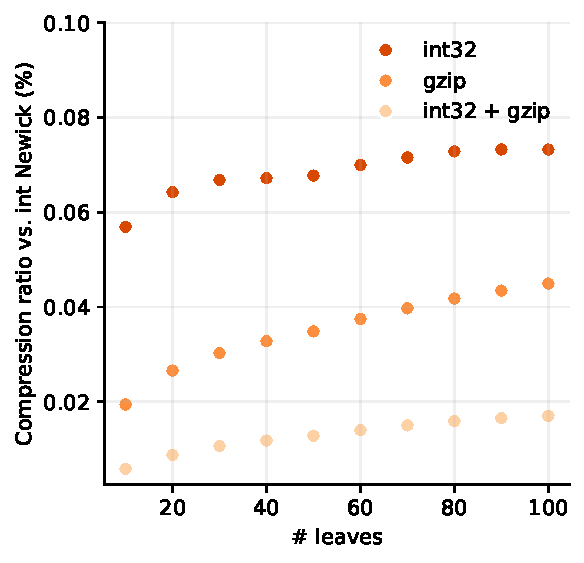
\includegraphics[width=0.4\textwidth]{img/p2v_vs_nwk_int_files.pdf}%
        \label{fig:p2v_vs_nwk_int_files}%
    }
    \hspace{0.25cm}
    \subfloat[]{%
        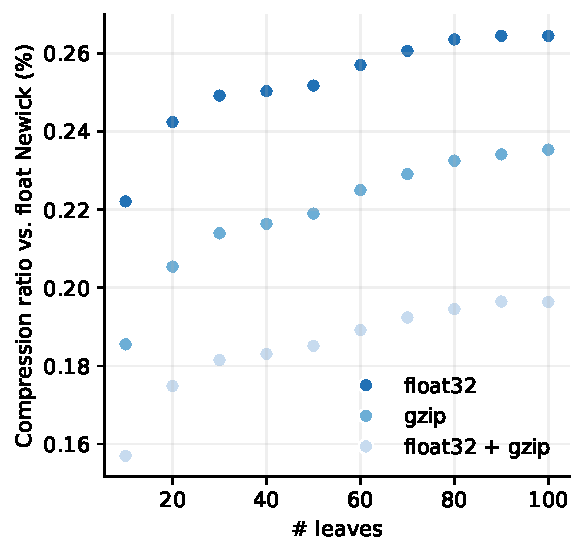
\includegraphics[width=0.4\textwidth]{img/p2v_vs_nwk_float_files.pdf}%
        \label{fig:p2v_vs_nwk_float_files}%
    }
    \caption{Analysing the compactness of the phylo2vec formats against the Newick format. \textsb{(a, b)}: compression ratia of tree topologies (resp. trees with branch lengths) as phylo2vec vectors (resp. as phylo2mat matrices) against their equivalent Newick strings. \textsb{(c, d)}: compression ratia of 10,000 random tree topologies (resp. trees with branch lengths) with coronavirus taxa saved as a plain-text file (often saved with the file extension \texttt{.trees}) vs. a hierarchical data format (HDF) file containing the trees as an array of phylo2vec vectors (resp. array of phylo2mat matrices), and a JSON representation of a mapping of taxon-to-integer labels. }
    \label{fig:p2v_compression}
\end{figure}

As a proof of concept, we demonstrated the feasibility of likelihood-based phylogenetic inference with phylo2vec using a hill-climbing scheme in Section~\ref{methods:p2v_inference} on four simple \glspl{msa}, three of which pertain to viral genes of Zika and Influenza A (Section~\ref{methods:p2v_evaluation}). The hill-climbing technique, which involves performing tree proposals using phylo2vec vectors and leveraging RAxML-NG~\cite{kozlov2019} for branch length and substitution optimisation based on the proposed vector, was generally able to recover a tree with the same likelihood as RAxML-NG used standalone~\cite{penn2025}. Despite starting from random trees, this scheme only required a fraction of tree proposals compared to the space of possible trees~\cite{penn2025}, thereby demonstrating that it can efficiently traverse tree space. However, our approach is more prone to being trapped in local optima due to the pulley principle~\cite{felsenstein2004}, whereby multiple rooted trees can have identical likelihoods when they represent different root placements of the same underlying topology. This creates optimisation challenges that are not typically encountered by most likelihood-based methods, which operate with unrooted trees~\cite{kozlov2019, minh2020}.

Overall, the simplicity of such a vector format makes it a convenient starting object for phylogenetic tree manipulation, as showcased in the \texttt{phylo2vec} software package~\cite{scheidwasser2025}. The package also highlights other potential avenues for phylo2vec-based phylogenetic inference, including scripts to calculate the likelihood of a phylo2mat matrix using BEAGLE~\cite{ayres2019} and non-traditional optimisation approaches such as (gradient-based \gls{bme} (GradME)~\cite{penn2023}).

\clearpage
\section{Summarized results from Study 2}
The overarching goal of this study was to evaluate the informational utility of structure-based phylogenetics to complement our understanding of viral evolution. To this end, we gathered experimental spike glycoprotein structures from the \gls{pdb}~\cite{berman2000, rose2010} of various species of the \textit{Betacoronavirus} genus. We used Foldseek~\cite{vankempen2024} to translate the structures into discrete sequences and MAST~\cite{wong2024} to analyse how recombination shapes the structural evolution of spike proteins.

Mixture modelling showed different classes in spike for RBD/NTD/S2.
Less precise with 3di, but similar pattern.

\clearpage
\section{Summarized results from Study 3}
The last study of this thesis aimed to detect infection in poultry using a deep learning-based framework to analyse animal behaviour from video data. To this end, we designed a pilot study to assess welfare impairments caused by \textit{E. coli} infection in broiler chickens~\cite{scheidwasser2024}. Two groups of 20 broiler chickens, one control group and one group infected with \textit{E. coli}, were monitored during the infection phase through video recordings. Using a deep neural network fine-tuned to track broilers, we extracted several kinematic features pertaining to behaviour, including distance travelled, change in body area, and time spent near the food source. Using validation data from optical flow and physiological biomarkers of inflammation, we provide a proof-of-concept that deep learning-based markerless tracking can be used for the early detection of infection in poultry cohorts. % We posit that this approach constitutes a noninvasive, scalable method to enhance flock health monitoring and biosecurity.

Post-mortem examination confirmed successful infection establishment. Chickens in the infected group, contrary to the control group, displayed hallmark physiological symptoms of acute infection, including lesions in multiple organs, elevated serum amyloid A (SAA) levels, and high bacterial \gls{cfu} levels~\cite{scheidwasser2024}.

Behavioural analysis using DeepLabCut-based tracking revealed substantial differences between the control and infected groups. Bayesian mixed-effects modelling showed that infected chickens were significantly less active than controls, with a 24\% reduction in distance travelled (95\% \gls{cri}: 6-39\%) and a 23\% reduction in body area change rate (95\% \gls{cri}: 4-39\%). Infected birds also spent 41\% less time near food sources (95\% \gls{cri}: 24-56\%), suggesting reduced feeding behaviour~\cite{scheidwasser2024}.

Subsequently, we compared the behavioural features obtained from animal tracking with optical flow, an established technique for monitoring welfare in poultry~\cite{dawkins2009, dawkins2012, colles2016, dawkins2017}. We observed a strong positive correlation with the average distance travelled by animals in videos ($r$ = 0.636, $p$ = 0.048), with control groups exhibiting higher mean optical flow and greater behavioural variance than infected animals~\cite{scheidwasser2024}. This result thus helped validate the plausibility of the tracking-based features as predictors of \textit{E. coli} infection.

Overall, the validation of this framework against physiological biomarkers and traditional optical flow analyses demonstrated its capability to effectively discriminate between healthy and infected birds. Notably, tracking-based features were sufficient to detect significant behavioural differences between groups within one day of infection~\cite{scheidwasser2024}. Although this study did not allow for tracking at the individual level due to the lack of preservation of animal identity across videos (see Section~\ref{methods:chicken_stats}), it constitutes a promising avenue for early disease detection in commercial settings.


Campy: ...

\chapter{Discussion}
In this thesis, we presented three studies pertaining to diverse, yet related facets of pandemic preparedness: The cornerstone of this thesis revolves around engineering new data formats and analysing of lesser explored datasets which may complement existing approaches to understanding the evolution and transmission of pathogenic diseases with epidemic potential. 

On the one hand, the overarching goal of phylo2vec was to provide a new bridge between the worlds of phylogenetics and machine learning through a compact vectorization of phylogenetic trees. Drawing inspiration from tree enumeration strategies~\cite{rohlf1983}, this study has breathed new life into the development of new vector-based representations of phylogenies such as HOP~\cite{chauve2025} and OLA~\cite{richman2025}.

% Currently limited scope beyond its compression/efficient representation/fast sampling, which are cool but not detrimental problems in phylogenetics. Could be a no free lunch thing, where operations are more difficult to imagine when you start from a vector that describes a branching process vs. an explicit tree itself. Although the new edition of the software in Rust/Python/R has more functionalities, the next step is likely to really dabble further into phylogenetic inference. Another possibility is data visualisation, but that would be a bit far from the original advantages of phylo2vec.

Nevertheless, the path to their usage in machine or deep learning applications relevant to epidemiology remains uncertain. In particular, it is unclear how an end-to-end deep neural network-based solution for general phylogenetic inference could be constructed~\cite{sapoval2022}. At its essence, deep learning requires a neural network and data from which the network learns from, and a metric to evaluate the learning performance. As an example, consider maximum likelihood-based molecular phylogenetic inference as a task to model with deep learning. Input data typically include an alignment of $n$ molecular sequence with $m$ sites and a model of evolution. Outputs are a single bifurcating tree and associated parameters which maximize Felsenstein's likelihood~\cite{felsenstein1973, felsenstein1981}. Although this metric may be adopted for deep learning-based applications, it is not fully differentiable due to the discreteness of tree topology, at least not without continuous relaxations~\cite{penn2023} or projections in non-Euclidean spaces~\cite{mimori2023, macaulay2024}. Furthermore, current approaches involving gradient computations on trees are not yet as efficient as precisely handcrafted approaches~\cite{fourment2023}. In addition, these approaches have not yet managed to fully leverage \glspl{gpu} to parallelize computations~\cite{fourment2023}, which is a hallmark of the success of deep learning~\cite{krizhevsky2012, lecun2015, vaswani2017}. Beyond issues related to tree likelihood, building comprehensive and biologically plausible training datasets is also non-trivial. In general, the validity of an inferred tree is inherently constrained by available data and models of evolution~\cite{yang2014}. In more specific cases involving reticulate processes (e.g., recombination), binary trees may provide an incomplete picture of evolutionary history~\cite{huson2006, wong2024}. To that end, several deep learning-based approaches have made use of simulated data from trees, but are yet to outperform likelihood-bases approaches~\cite{nesterenko2025}. Last, but most prominently, a deep learning approach would need to be both sufficiently flexible and scalable to incorporate a hugely variable-length input and predict an optimal tree from a combinatorially vast tree space~\cite{sapoval2022}. Various sequence representation approaches have been explored, including chaos game representations~\cite{jeffrey1990} and learnable representations from Transformer-based models~\cite{consens2025}. However, these approaches are yet to provide additional insight on evolution~\cite{reasoning}. Alternatively, graph-based generative models may also have potential for generating plausible trees~\cite{xie2023, xie2025}, but currently remain limited for practical phylogenetic applications. Consequently, an emerging body of research at the intersection of deep learning and phylogenetics has focused on optimising model parameters through tools like ModelTeller~\cite{abadi2020}, ModelFinder~\cite{kalyaanamoorthy2017}, and PhyloDeep~\cite{voznica2022}, which constitutes a promising avenue for phylo2vec usage.

Finally, the development of phylo2vec also motivated the development of a high-performance software for phylogenetic tree manipulation~\cite{scheidwasser2025}, comprising various functions for tree sampling, format conversions and operations on trees. However, key features are still lacking for the software to become a fully featured and widely adopted tool in the bioinformatics community. While the computational efficiency of the library may facilitate rapid tree visualisation, the non-equivalence of topology moves in the phylo2vec space to rooted \gls{spr} moves represents a promising avenue for the development of phylogenetic inference based on phylo2vec.

% Key features are still missing to make the software fully-fledged and attractive to the bioinformatics community, notably phylogenetic inference. 

% the super-exponential nature of tree space makes scalability a considerable challenge for deep learning-based solutions.

%  % First, ``true" evolutionary trees may be difficult or impossible to establish. For some loci or genes involving reticulate processes (e.g., recombination), binary trees may provide an incomplete picture of evolutionary history~\cite{huson2006, wong2024}. 

% Whereas 

% may be difficult or impossible to definitively establish, particularly when  are involved. simualtions

% % it is not immediately differentiable due to its recursive nature.

% However, building a comprehensive and plausible training dataset is nontrivial. \textcolor{red}{True trees may be difficult if not impossible to infer, e.g. in the case of reticulate processes (tree mixtures and phylo networks might be better). Second, what is a true tree anyway? Third, model of evolution?}. In addition, a deep learning approach would need to be both sufficiently flexible and scalable to incorporate a hugely variable-length input and predict a single tree from a potentially exponentially vast tree space. \textcolor{red}{chaos game representation for sequences~\cite{jeffrey1990}, representing sequences as text (hydra)}. \textcolor{red}{graphvae, graphrnn, diffusion have potential to generate trees/graphs (phylovae?)}, but they are poorly scalable. \textcolor{red}{phyloformer does not beat iqtree, and is worse as the number of sequences grows. gradme = not deep learning but gradient based, not better than iqtree.}. Thus, a body of research at the intersection of deep learning and phylogenetics is consacred to optimizing model parameters: ModelTeller, PhyloDeep~\cite{voznica2022} etc. This also constitutes a promising avenue for phylo2vec usage. \textcolor{red}{I have thought of MCTS for phylo2vec inference, but scalability remains an issue}.

The second study of this thesis aimed at exploring the potential added value of data from protein structures into giving insights on viral/pathogenic evolution. Mixed bag of results, difficult problem. Foldseek trained on a cluster of proteins and may not be fine-grained enough to accurately model all angles? 
% In molecular phylogenetic inference, input data typically consists of $N$ molecular sequences and the output typically consists of an optimal bifurcating tree (and associated parameters), or a distribution of trees in Bayesian phylogenetics.

% \textcolor{red}{chaos game representation}  with deterministic ...  On the one hand, 

% collecting a valid and comprehensive training dataset is a nontrivial task, as obtaining a ``true" bifurcating phylogeny may not be possible. For instance, reticulate processes of evolution such as horizontal gene transfer or recombination cannot accurately be modelled by inferring a single bifurcating tree. Instead, approaches based on mixtures of trees and phylogenetic networks have proved to be more insightful and plausible~\cite{huson2006, wong2024}. 

% is practically impossible, as obtaining a ``true" bifurcating phylogeny may not be possible

% A general deep learning solution would have to face face  due to scalability (tree space grows exponentially) and lack of training data (obtaining a ``true" bifurcating phylogeny is   promising avenue is the inference of model parameters

% Inspired by other tree labelling strategies~\cite{rohlf1983, dinh2010}

% exploring how lesser explored representations of pathogenic data may h

Summary of the results of the papers and their relation to international state-of-the-art research within the subject area
If required for the studies, information on ethical and legal permits and approvals
Conclusions and perspectives for further research

Despite claims that "we could AlphaFold our way through the next pandemic", I'm not sure. Folding tons of proteins remains expensive, whether with deep learning or x-ray crystallography. Like a lot of things with AI, it's easy to get 90\% there, but the real work is the last 10\%. For pandemic data, this is also the case; currently it's still a doubt whether these systems can help with variant-level/individual-level structures. Whereas there is undoubtedly some value in understanding the structure of antigens, its increased complexity compared to sequences might not provide significant benefits compared to sequence-based phylogenetics. Current research should focus on exploiting "rapid response to fast viral evolution with topology-assisted..." or fine-tuning either protein structure models or structure-discretizers such as 3di to single viruses. All in all, this is again a sign that there is not single tool to rule all pandemic problems.

From a scientific point of view, pandemic preparedness is hugely multi-faceted. And within each of these facets, the skill sets needed are also diverse. Take chicken study for instance: we have deep learning, videography, microbiology, veterinary science.

Video-based animal surveillance, although a nice concept, is incredibly difficult due to the number of degrees of freedom.

While optical flow is limited in resolution/precision, deep learning-based tracking is not yet ready for farm-scale/bird-scale environments, where 100/1000+ animals coexist. It has lots of potential, both from a public health and an economic perspective, but scability is currently the Achille's heel. My personal idea would be a two-camera system: one cheap one, where we could perform basic optical flow surveillance. If there are zones with (sustained) lower-than-average inactivity, a second camera hooked to raspberry pi + GPU for tracking tries to assess the welfare of the individual in this zone. This would be a "best of both worlds" strategy: we use cheap optical-flow as it's fast, and restrict the number of animals to track using deep learning. A robot is also envisageble, but that poses additional logistical issues + invasive.

This PhD illustrates the need for collaboration between all sorts of sciences, from agricultural scientists and veterinarians to lab technicians to computer scientists. For vets, there is a need to develop and openly share such data to advance the field. Problematic in industries due to ethical concerns + whistleblowing?

Vectorising pandemic data is in any case important because of the sheer volume of data we collect. Terabytes of video data for animal surveillance, terabytes of sequences for large-scale human genomic surveillance, terabytes of protein structures. Being able to efficiently compress data is green (less memory, less heat? etc.), and makes sharing data easier.

\chapter{Conclusion}

\clearpage
\begin{refcontext}
    \printbibliography
\end{refcontext}

\begin{appendix}
\addcontentsline{toc}{chapter}{Appendix}
\chapter{Articles included in this thesis}
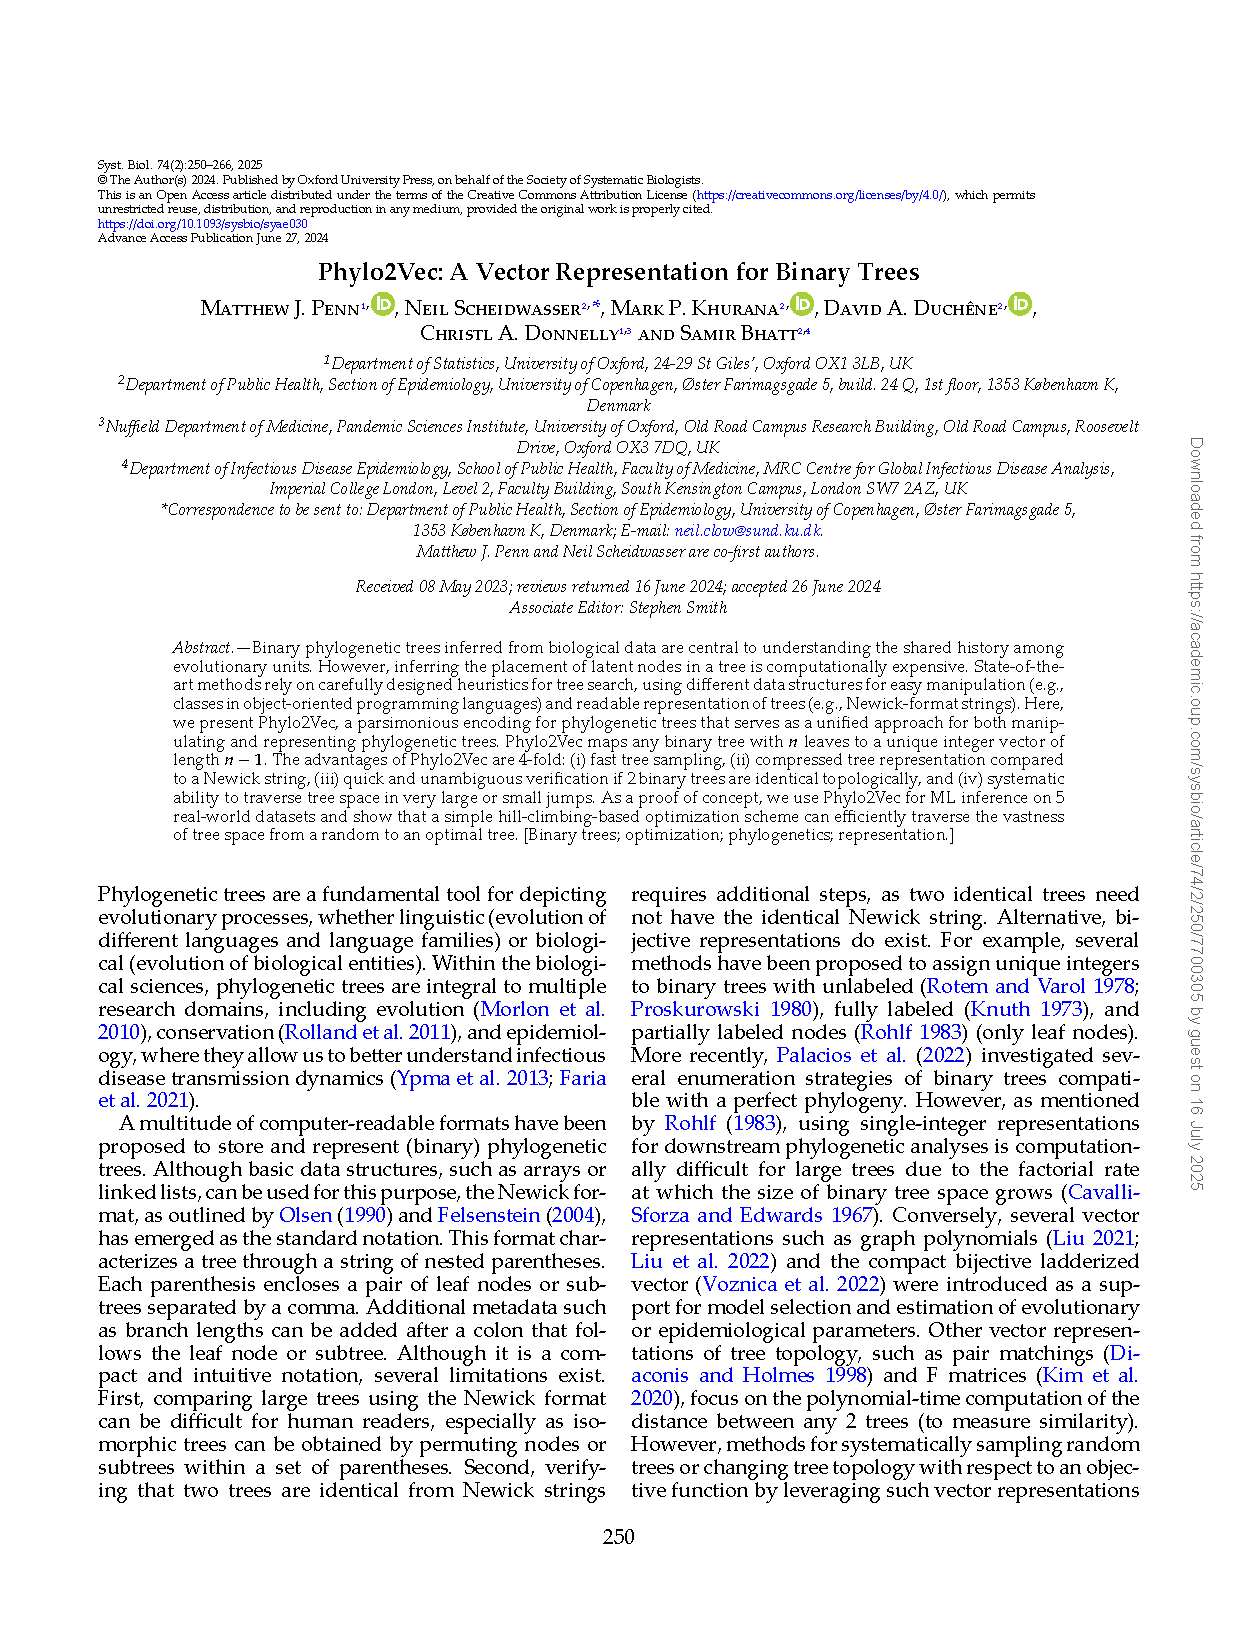
\includepdf[pages=-]{papers/phylo2vec_sysbio.pdf}
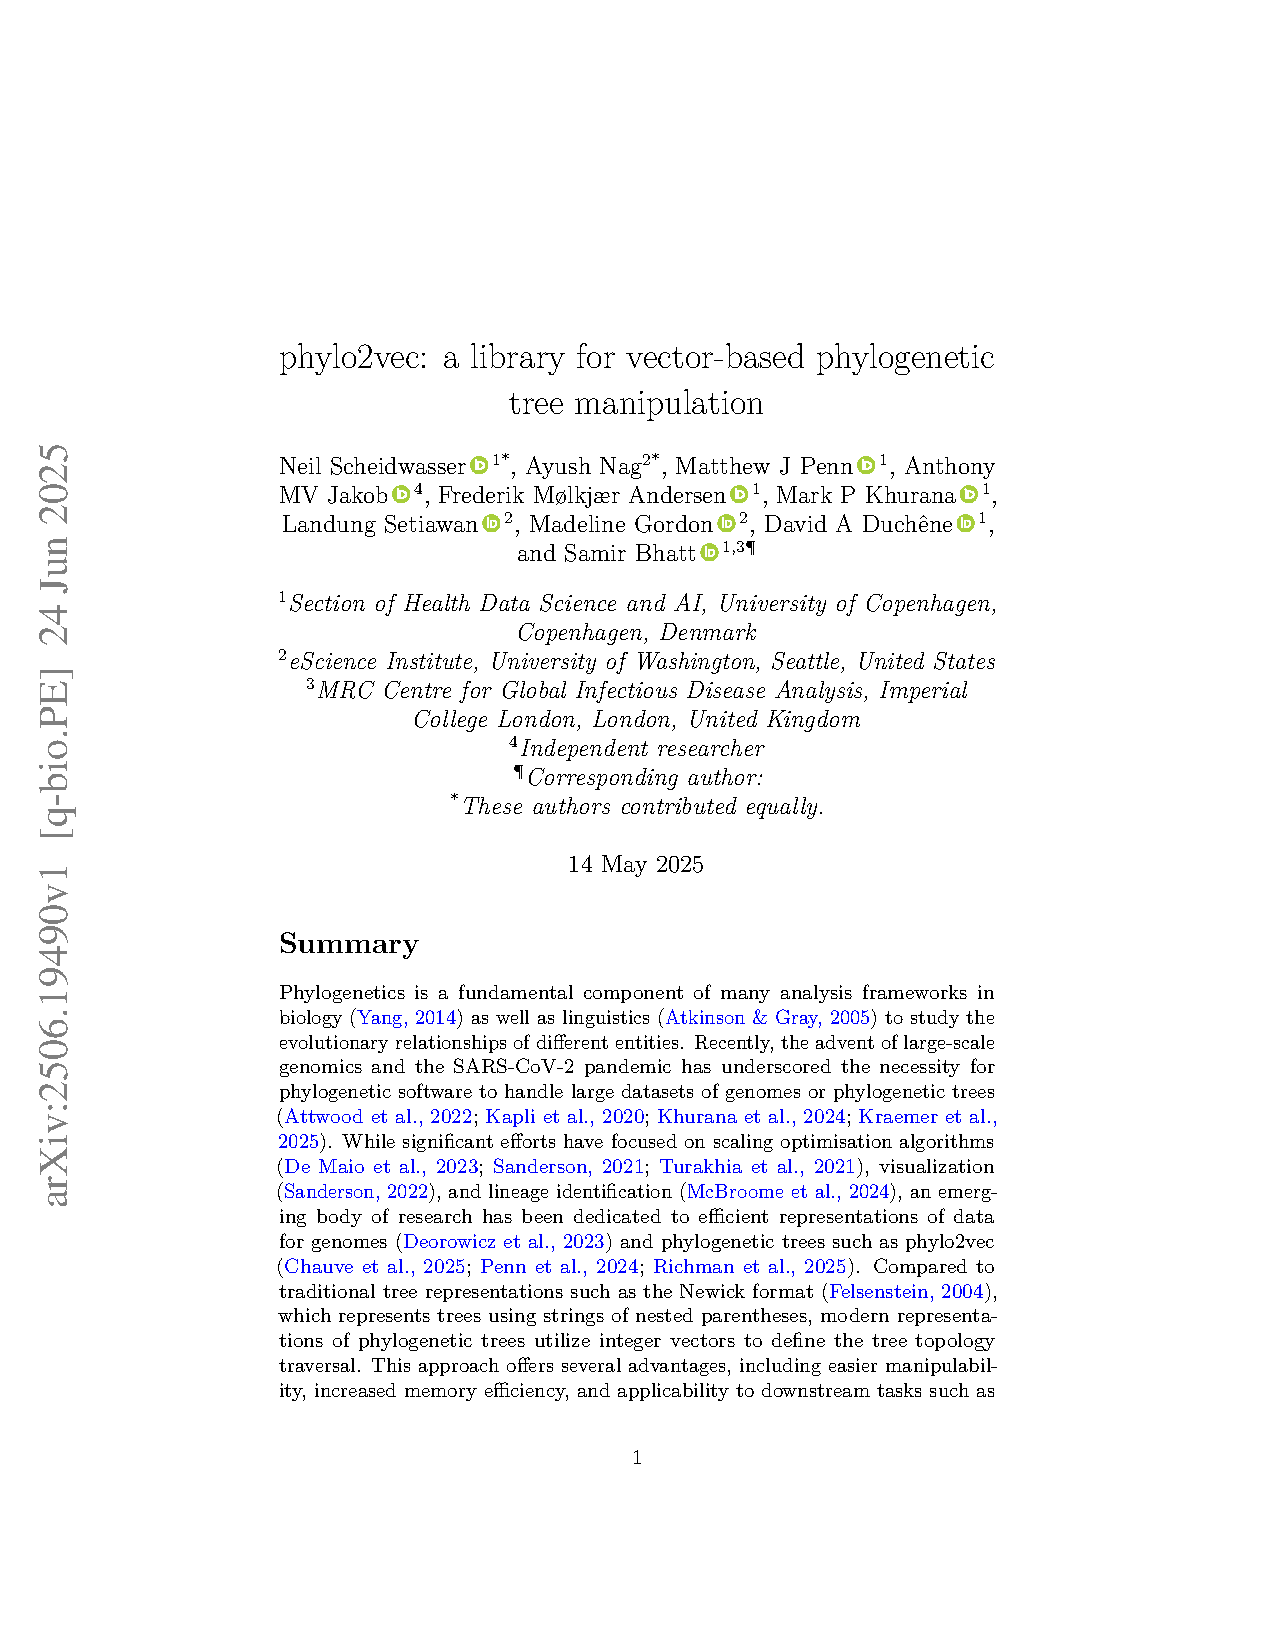
\includepdf[pages=-]{papers/phylo2vec_joss.pdf}
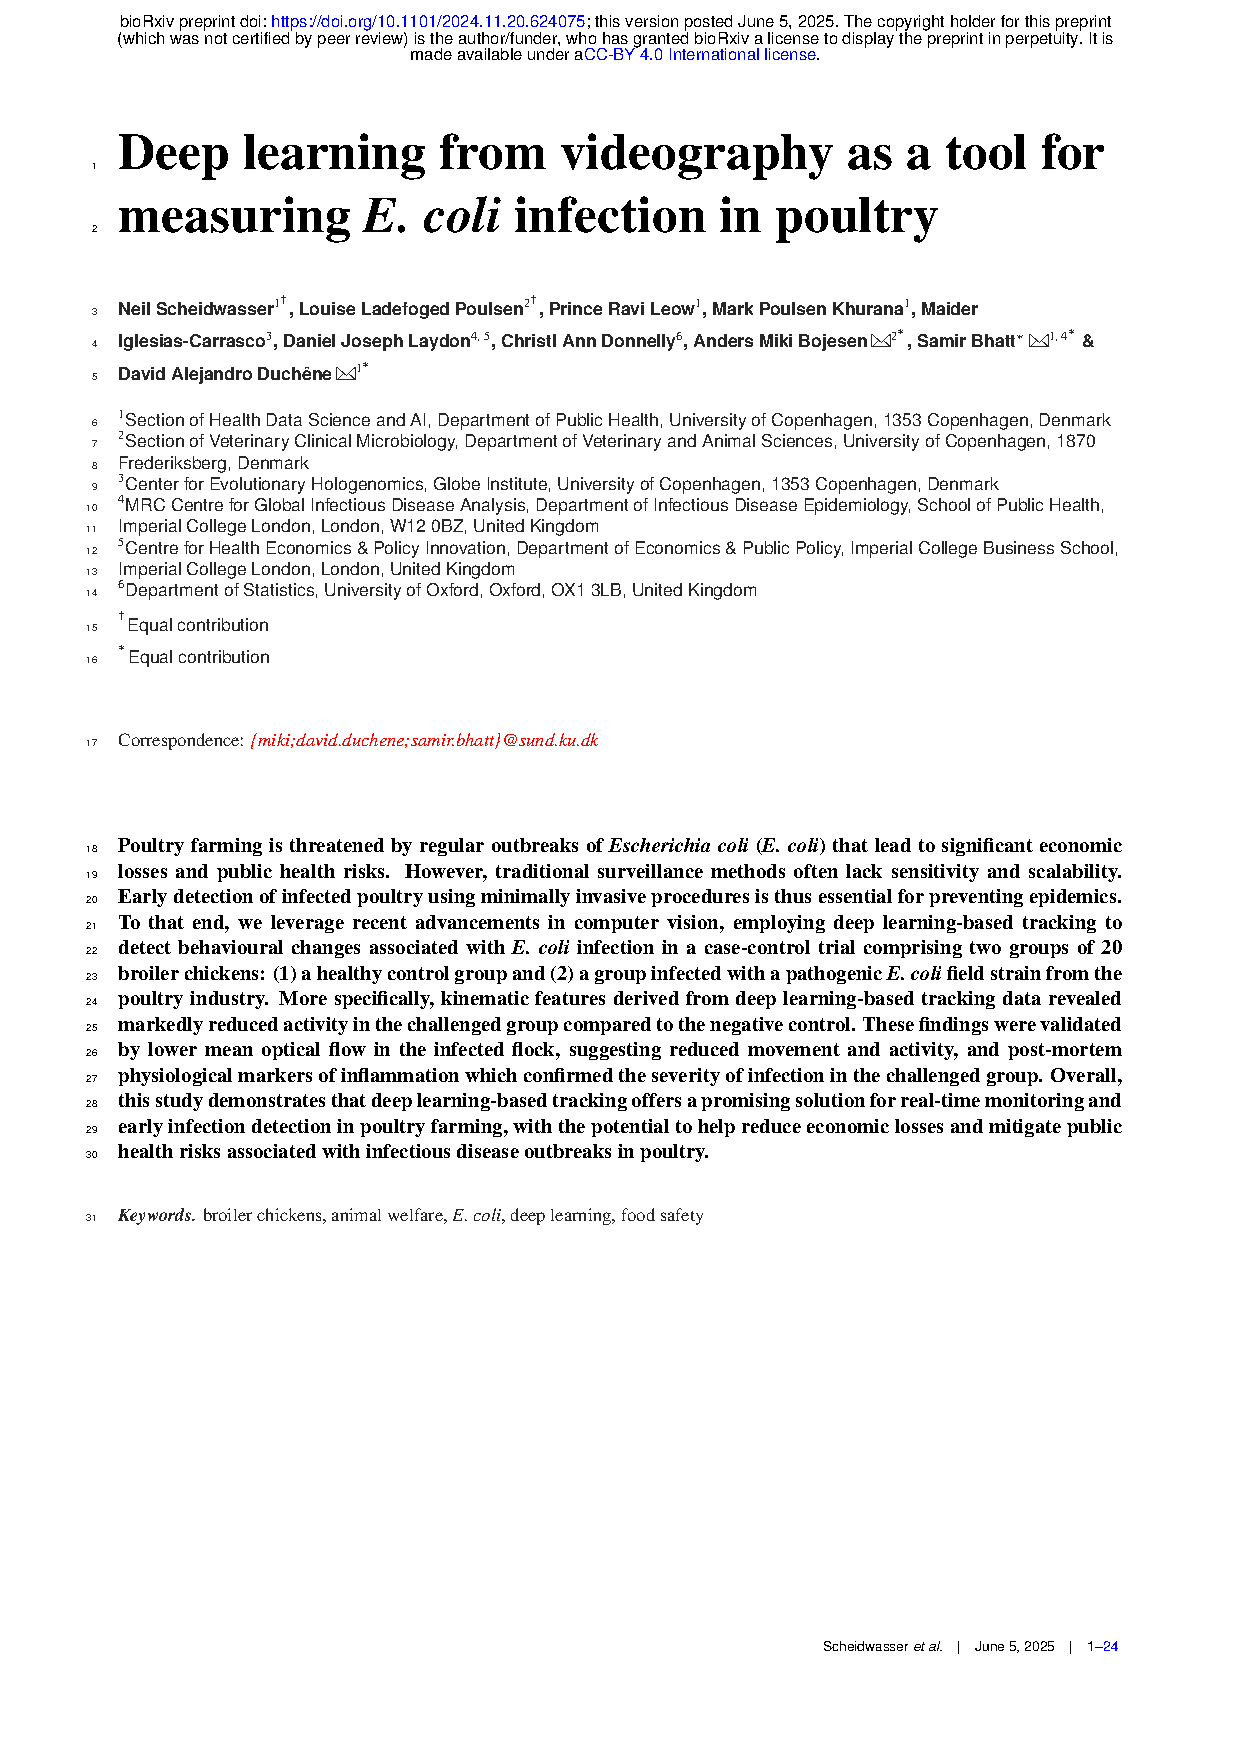
\includepdf[pages=-]{papers/chicken_ecoli.pdf}

\chapter{Co-authorship declaration}

\end{appendix}
\end{document}
